\documentclass[print]{dissertation}%for printing

\usepackage[utf8]{inputenc}
%for English
%\usepackage[english]{babel}
%for Vietnamese
\usepackage[vietnamese]{babel}

\usepackage{multirow}
\usepackage{listings}
\lstset{basicstyle=\ttfamily,escapechar=\@}
\usepackage{paralist}
\usepackage{graphicx}
\usepackage{wrapfig}
\usepackage{setspace}
\usepackage{amsthm}
\usepackage{array}
\usepackage{hyperref}
\hypersetup{colorlinks=true,pdfencoding=auto}
\usepackage{hypcap}
\usepackage{longtable}
\usepackage{rotating}
%\selectlanguage{vietnam}

\newcolumntype{L}[1]{>{\raggedright\let\newline\\\arraybackslash\hspace{0pt}}m{#1}}
\newcolumntype{C}[1]{>{\centering\let\newline\\\arraybackslash\hspace{0pt}}m{#1}}
\newcolumntype{R}[1]{>{\raggedleft\let\newline\\\arraybackslash\hspace{0pt}}m{#1}}

% Check / cross marks for comparison tables (using amssymb already loaded)
\newcommand{\cmark}{\ensuremath{\checkmark}}
\newcommand{\xmark}{\ensuremath{\times}}

%\newtheorem{interconnect}{Solution}
%\newtheorem{challenges}{Question}
%\newtheorem{taxonomy}{Taxonomy}
%\newtheorem{contribution}{Contribution}
\begin{document}
%\renewcommand{\baselinestretch}{1.2}\normalsize


%% Specify the title and author of the thesis. This information will be used on
%% the title page (in title/title.tex) and in the metadata of the final PDF.
%\title{Kiến trúc Máy tính}
%\begin{otherlanguage*}{vietnam}
%\author{Phạm Quốc Cường}{}
%\end{otherlanguage*}

%% Use Roman numerals for the page numbers of the title pages and table of
%% contents.
\frontmatter

\begin{titlepage}

\begin{tikzpicture}[remember picture,overlay,inner sep=0,outer sep=0]
     \draw[line width=4pt] ([xshift=-1.5cm,yshift=-2cm]current page.north east) coordinate (A)--([xshift=1.5cm,yshift=-2cm]current page.north west) coordinate(B)--([xshift=1.5cm,yshift=2cm]current page.south west) coordinate (C)--([xshift=-1.5cm,yshift=2cm]current page.south east) coordinate(D)--cycle;

     \draw ([yshift=0.5cm,xshift=-0.5cm]A)-- ([yshift=0.5cm,xshift=0.5cm]B)--
     ([yshift=-0.5cm,xshift=0.5cm]B) --([yshift=-0.5cm,xshift=-0.5cm]B)--([yshift=0.5cm,xshift=-0.5cm]C)--([yshift=0.5cm,xshift=0.5cm]C)--([yshift=-0.5cm,xshift=0.5cm]C)-- ([yshift=-0.5cm,xshift=-0.5cm]D)--([yshift=0.5cm,xshift=-0.5cm]D)--([yshift=0.5cm,xshift=0.5cm]D)--([yshift=-0.5cm,xshift=0.5cm]A)--([yshift=-0.5cm,xshift=-0.5cm]A)--([yshift=0.5cm,xshift=-0.5cm]A);


     \draw ([yshift=-0.3cm,xshift=0.3cm]A)-- ([yshift=-0.3cm,xshift=-0.3cm]B)--
     ([yshift=0.3cm,xshift=-0.3cm]B) --([yshift=0.3cm,xshift=0.3cm]B)--([yshift=-0.3cm,xshift=0.3cm]C)--([yshift=-0.3cm,xshift=-0.3cm]C)--([yshift=0.3cm,xshift=-0.3cm]C)-- ([yshift=0.3cm,xshift=0.3cm]D)--([yshift=-0.3cm,xshift=0.3cm]D)--([yshift=-0.3cm,xshift=-0.3cm]D)--([yshift=0.3cm,xshift=-0.3cm]A)--([yshift=0.3cm,xshift=0.3cm]A)--([yshift=-0.3cm,xshift=0.3cm]A);

\end{tikzpicture}

\begin{center}

%% Extra whitespace at the top.
%\vspace*{2\bigskipamount}

%%print author name
%\begin{otherlanguage*}{vietnamese}
\makeatletter
{\large\titlefont\bfseries ĐẠI HỌC QUỐC GIA THÀNH PHỐ HỒ CHÍ MINH}\\
{\large\titlefont\bfseries TRƯỜNG ĐẠI HỌC BÁCH KHOA}\\
{\large\titlefont\bfseries KHOA KHOA HỌC VÀ KỸ THUẬT MÁY TÍNH}

%{\Large\titlefont\bfseries\@firstname\ {\titleshape\@lastname}}
\makeatother
%\end{otherlanguage*}

\begin{center}

\includegraphics[width=3cm]{hcmut.png}
\end{center}

\vspace{1 cm}
%% Print the title.
{\makeatletter
\large\titlestyle ĐỒ ÁN TỐT NGHIỆP\\
\vspace{0.5cm}
\titlestyle\bfseries\LARGE phát triển platform edge-ai dựa trên fpga sử dụng risc-v\\
\vspace{1cm}
\large\titlestyle Ngành: KỸ THUẬT MÁY TÍNH\\
\titlestyle Hội đồng: xx
\makeatother}

\vspace{0.75cm}

\begin{table}[h!]
\begin{tabular}{lll}
\hspace{1cm}
& \hspace{-0.5 cm} \vspace{0.25cm} \textbf{Người hướng dẫn}: &\\
& PGS. TS. Phạm Quốc Cường &- Trường ĐHBK\\
\vspace{0.25cm} & <Name> &- <affiliation>\\ 
& \hspace{-0.5 cm} \vspace{0.25cm} \textbf{Người Phản biên}: &\\
\vspace{0.25cm} & Assoc. Prof. Dr. <name> &- HCMUT\\
& \hspace{-0.5 cm} \vspace{0.25cm} \textbf{Sinh viên thực hiện}: &\\
\vspace{0.25cm} & Nguyễn Trung Tân &- 2213063\\
\vspace{0.25cm} & Trần Minh Tâm &- 2213039\\
\end{tabular}
\end{table}

\vfill

%{\Large\titlefont\bfseries NHÀ XUẤT BẢN ĐẠI HỌC QUỐC GIA}\\
{\titlefont\bfseries THÀNH PHỐ HỒ CHÍ MINH - THÁNG 5 NĂM 2026}
\end{center}

\cleardoublepage
\thispagestyle{empty}


\clearpage
\thispagestyle{empty}
%% The following line is dictated by the promotieregelement.
%\noindent Dit proefschrift is goedgekeurd door de promotor:

\end{titlepage}



%% The (optional) dedication can be used to thank someone or display a
%% significant quotation.
%\dedication{\epigraph{To my wife and my son}{}}
\dedication{\epigraph{This thesis is dedicated for our parents and our instructors at HCMUT.}{}}

%\include{preface/ack}
%\chapter{Lời cảm ơn}
%\addcontentsline{toc}{chapter}{Abstract}
\setheader{Lời cảm ơn}

Việc hoàn thành đồ án này không chỉ là kết quả của sự nỗ lực từ phía nhóm thực hiện, mà còn là sự kết tinh từ sự chỉ dẫn tận tình và động viên to lớn của quý thầy cô, gia đình và bạn bè.

Lời tri ân sâu sắc nhất, chúng tôi xin được gửi tới Thầy Phạm Quốc Cường. Thầy không chỉ là người hướng dẫn khoa học, định hướng cho chúng tôi những lối đi đúng đắn trong mê cung kiến thức, mà còn là người truyền lửa, giúp chúng tôi kiên trì vượt qua những rào cản kỹ thuật hóc búa trong suốt quá trình thực hiện đề tài. Những kinh nghiệm quý báu mà Thầy chia sẻ thực sự là hành trang vô giá đối với chúng tôi.

Chúng tôi cũng xin bày tỏ lòng biết ơn chân thành đến Quý Thầy Cô thuộc Khoa Khoa học và Kỹ thuật Máy tính, Trường Đại học Bách Khoa - ĐHQG TP.HCM. Môi trường học thuật nghiêm túc và nền tảng kiến thức vững chắc mà các Thầy Cô đã dày công vun đắp chính là bệ phóng để chúng tôi có thể tự tin giải quyết các vấn đề trong đồ án này cũng như trong sự nghiệp sau này.

Cuối cùng, xin gửi lời cảm ơn đến gia đình – hậu phương vững chắc nhất, và những người bạn đã luôn sát cánh, chia sẻ khó khăn. Sự ủng hộ của mọi người chính là nguồn động lực tinh thần to lớn giúp chúng tôi đi đến cuối hành trình này.

Xin chân thành cảm ơn!

\chapter{Tóm tắt}
%\addcontentsline{toc}{chapter}{Abstract}
\setheader{Tóm tắt}

Trong kỷ nguyên số hóa, Internet vạn vật (IoT) đã chuyển mình từ một khái niệm công nghệ trở thành hạ tầng thiết yếu của đời sống hiện đại. Từ các thiết bị dân dụng như Smart TV đến các mạng lưới cảm biến công nghiệp phức tạp, IoT đang tạo ra một lượng dữ liệu khổng lồ. Xu hướng tất yếu hiện nay là tích hợp Trí tuệ nhân tạo (AI) vào các thiết bị này để tạo nên AIoT (Artificial Intelligence of Things), giúp thiết bị không chỉ ``kết nối'' mà còn có khả năng ``tư duy''.

Tuy nhiên, việc triển khai AI trên các thiết bị IoT truyền thống đang vấp phải ``nút thắt cổ chai'' về kiến trúc. Mô hình phổ biến hiện nay dựa vào việc đẩy dữ liệu lên máy chủ đám mây (Cloud Server) để xử lý tập trung. Mô hình này bộc lộ nhiều điểm yếu chí mạng: rủi ro gián đoạn dịch vụ khi mất kết nối mạng, độ trễ cao không phù hợp cho các ứng dụng thời gian thực, và gánh nặng băng thông lớn.

Về mặt phần cứng, các vi xử lý (CPU) thương mại từ các hãng lớn, dù mạnh mẽ, thường gặp vấn đề về tiêu thụ năng lượng khi phải gồng gánh các tác vụ AI liên tục. Hơn nữa, tính chất đóng kín của các dòng chip này khiến các nhà phát triển gặp khó khăn trong việc tùy biến sâu để tối ưu hóa hiệu năng cho các thuật toán AI cụ thể, đồng thời rào cản chi phí bản quyền cũng là một trở ngại lớn cho đổi mới sáng tạo.

Sự xuất hiện của RISC-V đã mang đến một luồng gió mới cho ngành công nghiệp bán dẫn. Là một kiến trúc tập lệnh mở (Open ISA), RISC-V phá bỏ thế độc quyền của các kiến trúc đóng, trao quyền cho các tổ chức nhỏ, các nhóm nghiên cứu và cá nhân khả năng tự thiết kế các lõi CPU chuẩn hóa. Ưu điểm vượt trội của RISC-V nằm ở tính mô-đun hóa và khả năng mở rộng. Các kỹ sư có thể tự do thêm các tập lệnh tùy chỉnh hoặc sửa đổi vi kiến trúc để phục vụ cho các tác vụ chuyên biệt mà không vướng phải rào cản pháp lý hay chi phí bản quyền đắt đỏ. Đây chính là chìa khóa để giải quyết bài toán hiệu năng/năng lượng cho các thiết bị IoT thế hệ mới.

Dựa trên những phân tích trên, dự án của nhóm tập trung phát triển một nền tảng Edge-AI (AI tại biên) chuyên dụng, lấy kiến trúc RISC-V làm nòng cốt. Mục tiêu của nhóm không chỉ dừng lại ở việc sử dụng một lõi CPU đa năng. Thay vào đó, nhóm tận dụng khả năng tùy biến của RISC-V để thiết kế một hệ thống tích hợp sâu, bao gồm một lõi xử lý trung tâm được tối ưu hóa (CV32E40P, RV32IMC) kết hợp với một bộ tăng tốc CNN tùy chỉnh (Conv-CNN v2.0) tự thiết kế bằng SystemVerilog ở mức RTL. Hệ thống được hiện thực trên nền tảng Xilinx Kria KV260 (Zynq UltraScale+) theo kiến trúc dị thể (heterogeneous): lõi ARM Cortex-A53 chạy Ubuntu PYNQ đảm nhiệm vai trò host, lõi RISC-V điều phối luồng tính toán bare-metal, và bộ tăng tốc thực thi tích chập INT8.

Mô hình \texttt{Tiny-VGG} (5 lớp Conv $3\times3$, $\sim$25.7K tham số INT8) được huấn luyện và lượng tử hóa theo chuẩn TFLite cho bài toán phân loại nhị phân \textit{Cats vs Dogs}, đạt độ chính xác \textbf{79.38\% (FP32) / 79.53\% (INT8)} trên tập validation 5{,}000 ảnh -- phương pháp PTQ không gây tổn thất đáng kể (chênh lệch $+0.15\%$ trong ngưỡng nhiễu thống kê). Riêng việc bổ sung 3 kỹ thuật augmentation (flip + crop + brightness/contrast) đem lại $+5.50\%$ accuracy so với baseline không augment.

Về phần cứng, hệ thống tổng hợp thành công trên Vivado 2025.2.1 với tài nguyên sử dụng ở mức rất thấp: \textbf{19.20\% LUT} (22{,}491 / 117{,}120), \textbf{12.26\% FF}, \textbf{0.72\% DSP} (chỉ 9 / 1{,}248 — chính xác bằng số PE MAC), \textbf{68.75\% BRAM}; Worst Negative Slack đạt $+2.118$~ns ở tần số 100~MHz (Fmax thực tế $\sim$127~MHz, dư địa lớn cho mở rộng tương lai). Tổng công suất ước tính \textbf{2.945~W}, trong đó toàn bộ logic người dùng PL chỉ tốn $\sim$0.225~W -- riêng bộ gia tốc \texttt{conv\_cnn\_0} chỉ tiêu thụ \textbf{23~mW}.

Đề tài định vị ở phân khúc \textit{open-source, loosely-coupled, INT8, có RISC-V orchestrator} -- một phân khúc chưa được lấp đầy bởi các framework hiện có (Vitis AI DPU, FINN, hls4ml, CFU Playground). Toàn bộ mã nguồn (RTL, firmware, host runtime, training pipeline) được phát hành mở, phù hợp cho mục đích nghiên cứu và giảng dạy về thiết kế hệ thống nhúng AI.


% \chapter{Abstract}
% %\addcontentsline{toc}{chapter}{Abstract}
% \setheader{Abstract}

% Write your abstract in English here




\tableofcontents
\listoffigures
\listoftables
%% Use Arabic numerals for the page numbers of the chapters.
\chapter{Lời cảm ơn}
%\addcontentsline{toc}{chapter}{Abstract}
\setheader{Lời cảm ơn}

Việc hoàn thành đồ án này không chỉ là kết quả của sự nỗ lực từ phía nhóm thực hiện, mà còn là sự kết tinh từ sự chỉ dẫn tận tình và động viên to lớn của quý thầy cô, gia đình và bạn bè.

Lời tri ân sâu sắc nhất, chúng tôi xin được gửi tới Thầy Phạm Quốc Cường. Thầy không chỉ là người hướng dẫn khoa học, định hướng cho chúng tôi những lối đi đúng đắn trong mê cung kiến thức, mà còn là người truyền lửa, giúp chúng tôi kiên trì vượt qua những rào cản kỹ thuật hóc búa trong suốt quá trình thực hiện đề tài. Những kinh nghiệm quý báu mà Thầy chia sẻ thực sự là hành trang vô giá đối với chúng tôi.

Chúng tôi cũng xin bày tỏ lòng biết ơn chân thành đến Quý Thầy Cô thuộc Khoa Khoa học và Kỹ thuật Máy tính, Trường Đại học Bách Khoa - ĐHQG TP.HCM. Môi trường học thuật nghiêm túc và nền tảng kiến thức vững chắc mà các Thầy Cô đã dày công vun đắp chính là bệ phóng để chúng tôi có thể tự tin giải quyết các vấn đề trong đồ án này cũng như trong sự nghiệp sau này.

Cuối cùng, xin gửi lời cảm ơn đến gia đình – hậu phương vững chắc nhất, và những người bạn đã luôn sát cánh, chia sẻ khó khăn. Sự ủng hộ của mọi người chính là nguồn động lực tinh thần to lớn giúp chúng tôi đi đến cuối hành trình này.

Xin chân thành cảm ơn!

\chapter{Tóm tắt}
%\addcontentsline{toc}{chapter}{Abstract}
\setheader{Tóm tắt}

Trong kỷ nguyên số hóa, Internet vạn vật (IoT) đã chuyển mình từ một khái niệm công nghệ trở thành hạ tầng thiết yếu của đời sống hiện đại. Từ các thiết bị dân dụng như Smart TV đến các mạng lưới cảm biến công nghiệp phức tạp, IoT đang tạo ra một lượng dữ liệu khổng lồ. Xu hướng tất yếu hiện nay là tích hợp Trí tuệ nhân tạo (AI) vào các thiết bị này để tạo nên AIoT (Artificial Intelligence of Things), giúp thiết bị không chỉ ``kết nối'' mà còn có khả năng ``tư duy''.

Tuy nhiên, việc triển khai AI trên các thiết bị IoT truyền thống đang vấp phải ``nút thắt cổ chai'' về kiến trúc. Mô hình phổ biến hiện nay dựa vào việc đẩy dữ liệu lên máy chủ đám mây (Cloud Server) để xử lý tập trung. Mô hình này bộc lộ nhiều điểm yếu chí mạng: rủi ro gián đoạn dịch vụ khi mất kết nối mạng, độ trễ cao không phù hợp cho các ứng dụng thời gian thực, và gánh nặng băng thông lớn.

Về mặt phần cứng, các vi xử lý (CPU) thương mại từ các hãng lớn, dù mạnh mẽ, thường gặp vấn đề về tiêu thụ năng lượng khi phải gồng gánh các tác vụ AI liên tục. Hơn nữa, tính chất đóng kín của các dòng chip này khiến các nhà phát triển gặp khó khăn trong việc tùy biến sâu để tối ưu hóa hiệu năng cho các thuật toán AI cụ thể, đồng thời rào cản chi phí bản quyền cũng là một trở ngại lớn cho đổi mới sáng tạo.

Sự xuất hiện của RISC-V đã mang đến một luồng gió mới cho ngành công nghiệp bán dẫn. Là một kiến trúc tập lệnh mở (Open ISA), RISC-V phá bỏ thế độc quyền của các kiến trúc đóng, trao quyền cho các tổ chức nhỏ, các nhóm nghiên cứu và cá nhân khả năng tự thiết kế các lõi CPU chuẩn hóa. Ưu điểm vượt trội của RISC-V nằm ở tính mô-đun hóa và khả năng mở rộng. Các kỹ sư có thể tự do thêm các tập lệnh tùy chỉnh hoặc sửa đổi vi kiến trúc để phục vụ cho các tác vụ chuyên biệt mà không vướng phải rào cản pháp lý hay chi phí bản quyền đắt đỏ. Đây chính là chìa khóa để giải quyết bài toán hiệu năng/năng lượng cho các thiết bị IoT thế hệ mới.

Dựa trên những phân tích trên, dự án của nhóm tập trung phát triển một nền tảng Edge-AI (AI tại biên) chuyên dụng, lấy kiến trúc RISC-V làm nòng cốt. Mục tiêu của nhóm không chỉ dừng lại ở việc sử dụng một lõi CPU đa năng. Thay vào đó, nhóm tận dụng khả năng tùy biến của RISC-V để thiết kế một hệ thống tích hợp sâu, bao gồm một lõi xử lý trung tâm được tối ưu hóa (CV32E40P, RV32IMC) kết hợp với một bộ tăng tốc CNN tùy chỉnh (Conv-CNN v2.0) tự thiết kế bằng SystemVerilog ở mức RTL. Hệ thống được hiện thực trên nền tảng Xilinx Kria KV260 (Zynq UltraScale+) theo kiến trúc dị thể (heterogeneous): lõi ARM Cortex-A53 chạy Ubuntu PYNQ đảm nhiệm vai trò host, lõi RISC-V điều phối luồng tính toán bare-metal, và bộ tăng tốc thực thi tích chập INT8.

Mô hình \texttt{Tiny-VGG} (5 lớp Conv $3\times3$, $\sim$25.7K tham số INT8) được huấn luyện và lượng tử hóa theo chuẩn TFLite cho bài toán phân loại nhị phân \textit{Cats vs Dogs}, đạt độ chính xác \textbf{79.38\% (FP32) / 79.53\% (INT8)} trên tập validation 5{,}000 ảnh -- phương pháp PTQ không gây tổn thất đáng kể (chênh lệch $+0.15\%$ trong ngưỡng nhiễu thống kê). Riêng việc bổ sung 3 kỹ thuật augmentation (flip + crop + brightness/contrast) đem lại $+5.50\%$ accuracy so với baseline không augment.

Về phần cứng, hệ thống tổng hợp thành công trên Vivado 2025.2.1 với tài nguyên sử dụng ở mức rất thấp: \textbf{19.20\% LUT} (22{,}491 / 117{,}120), \textbf{12.26\% FF}, \textbf{0.72\% DSP} (chỉ 9 / 1{,}248 — chính xác bằng số PE MAC), \textbf{68.75\% BRAM}; Worst Negative Slack đạt $+2.118$~ns ở tần số 100~MHz (Fmax thực tế $\sim$127~MHz, dư địa lớn cho mở rộng tương lai). Tổng công suất ước tính \textbf{2.945~W}, trong đó toàn bộ logic người dùng PL chỉ tốn $\sim$0.225~W -- riêng bộ gia tốc \texttt{conv\_cnn\_0} chỉ tiêu thụ \textbf{23~mW}.

Đề tài định vị ở phân khúc \textit{open-source, loosely-coupled, INT8, có RISC-V orchestrator} -- một phân khúc chưa được lấp đầy bởi các framework hiện có (Vitis AI DPU, FINN, hls4ml, CFU Playground). Toàn bộ mã nguồn (RTL, firmware, host runtime, training pipeline) được phát hành mở, phù hợp cho mục đích nghiên cứu và giảng dạy về thiết kế hệ thống nhúng AI.


% \chapter{Abstract}
% %\addcontentsline{toc}{chapter}{Abstract}
% \setheader{Abstract}

% Write your abstract in English here



\mainmatter

%% Turn on thumb indices.
\thumbtrue

\chapter{Giới thiệu đề tài}
\label{chp:01}

Sự bùng nổ của AI và rào cản phần cứng Trong thập kỷ qua, thế giới đã chứng kiến sự chuyển mình mạnh mẽ của cuộc Cách mạng Công nghiệp 4.0, trong đó Trí tuệ nhân tạo (AI) đóng vai trò là động lực cốt lõi. Đặc biệt, sự ra đời của các mô hình ngôn ngữ lớn (LLMs) như ChatGPT đã đánh dấu một bước ngoặt lịch sử, đưa AI từ các ứng dụng nghiên cứu hẹp sang kỷ nguyên của AI tạo sinh (Generative AI) với khả năng tác động sâu rộng đến mọi mặt của đời sống xã hội. Tuy nhiên, đi cùng với tiềm năng to lớn đó là những thách thức chưa từng có về mặt hạ tầng tính toán. Các thuật toán AI hiện đại ngày càng trở nên phức tạp, đòi hỏi khả năng xử lý dữ liệu song song khổng lồ và băng thông bộ nhớ lớn. Điều này đã đẩy các kiến trúc vi xử lý truyền thống đến giới hạn của định luật Moore, gây ra các vấn đề nghiêm trọng về tiêu thụ năng lượng và độ trễ khi triển khai trên diện rộng.\\
\\
Mô hình xử lý AI tập trung trên đám mây hiện nay đang bộc lộ nhiều điểm yếu, bao gồm độ trễ đường truyền, rủi ro về bảo mật dữ liệu riêng tư và sự phụ thuộc vào kết nối Internet liên tục. Do đó, xu hướng công nghệ đang dịch chuyển mạnh mẽ sang tính toán tại biên (Edge Computing). Việc đưa AI xuống chạy trực tiếp trên các thiết bị cuối (Edge devices) đòi hỏi phần cứng không chỉ mạnh mẽ mà còn phải tiết kiệm năng lượng và chi phí thấp – một bài toán khó đối với các dòng chip thương mại đóng kín (proprietary chips) hiện có trên thị trường.\\
\\
Sự trỗi dậy của RISC-V Giữa bối cảnh "nút thắt cổ chai" về phần cứng đó, sự xuất hiện của kiến trúc tập lệnh mở RISC-V được xem là một cuộc cách mạng trong ngành bán dẫn. Khác với các kiến trúc đóng như x86 hay ARM vốn đòi hỏi chi phí bản quyền đắt đỏ và không cho phép can thiệp sâu vào thiết kế lõi, RISC-V mang đến sự tự do hoàn toàn. Điểm ưu việt nhất của RISC-V là tính mô-đun hóa  và khả năng mở rộng. Nó cho phép các kỹ sư thiết kế có thể thêm vào các tập lệnh tùy chỉnh để tối ưu hóa đặc biệt cho các tác vụ AI cụ thể, giúp tăng hiệu suất xử lý lên nhiều lần trong khi vẫn giữ mức tiêu thụ năng lượng ở mức thấp.\\
\\
Sự kết hợp RISC-V và công nghệ FPGA Để hiện thực hóa sức mạnh của RISC-V mà không cần tốn kém chi phí sản xuất chip silicon ngay từ đầu, công nghệ FPGA đóng vai trò là nền tảng phát triển lý tưởng. FPGA cho phép chúng ta thiết kế, kiểm thử và tái cấu hình phần cứng một cách linh hoạt như phần mềm. Sự kết hợp giữa khả năng tùy biến của RISC-V và tính linh hoạt của FPGA tạo điều kiện thuận lợi để xây dựng các dòng chip chuyên biệt hóa dành cho AI.

\section{Mục tiêu đề tài}
Mục tiêu tổng quát của đồ án là thiết kế, hiện thực và đánh giá một Nền tảng tính toán biên (Edge-AI Platform) hoàn chỉnh trên FPGA Kria KV260, ứng dụng kiến trúc Đa xử lý Bất đối xứng (AMP - Asymmetric Multiprocessing). Hệ thống là sự kết hợp giữa khả năng quản lý linh hoạt của vi xử lý Host (ARM Cortex-A53) và sức mạnh xử lý luồng dữ liệu chuyên biệt của lõi RISC-V, tạo ra một hệ sinh thái toàn diện từ phần cứng đến phần mềm để thực thi các mạng nơ-ron nhân tạo.

Các mục tiêu cụ thể bao gồm:
\begin{itemize}
    \item \textbf{Nghiên cứu kiến trúc SoC và lõi RISC-V:} Phân tích kiến trúc hệ thống xử lý (Processing System) của Zynq UltraScale+ và tổ chức lõi xử lý mã nguồn mở RISC-V CV32E40P. Tùy biến và triển khai thành công lõi RISC-V lên vùng logic khả trình (PL) của FPGA để hoạt động như một bộ gia tốc phần mềm (Software Accelerator) độc lập.

    \item \textbf{Làm chủ và tối ưu giao tiếp Memory Map:} Thiết kế hệ thống bus liên kết (Interconnect) dựa trên chuẩn AMBA AXI4. Trọng tâm là xây dựng cơ chế giao tiếp và đồng bộ hóa dữ liệu tốc độ cao giữa lõi ARM và RISC-V thông qua bộ nhớ chia sẻ (Shared BRAM), giải quyết bài toán nút thắt cổ chai dữ liệu (Data Bottleneck).

    \item \textbf{Phát triển Firmware và Quy trình Đồng thiết kế (HW/SW Co-design):} Phát triển phần mềm quản lý lớp ứng dụng trên hệ điều hành Linux (Host) và tối ưu hóa firmware C bare-metal cho lõi RISC-V. Ứng dụng các tập lệnh mở rộng để thực thi hiệu quả các phép toán ma trận của mạng CNN nhằm giảm tải cho vi xử lý trung tâm.

    \item \textbf{Pipeline huấn luyện và biên dịch mô hình:} Xây dựng pipeline huấn luyện mạng \texttt{vgg-tiny} INT8 trên Host PC, kết hợp với trình biên dịch tự sinh layer table (\texttt{layer\_table.h}) và blob trọng số (\texttt{weights.bin}) -- cho phép thay đổi mô hình AI mà không cần tổng hợp lại RTL. Pipeline hỗ trợ hai dataset chuẩn: Cats vs Dogs (Kaggle) và INRIA Person.

    \item \textbf{Tích hợp và Đánh giá hệ thống:} Triển khai toàn bộ nền tảng và kiểm chứng bằng pipeline phân loại nhị phân (binary classification) với mô hình \texttt{vgg-tiny} (5 conv layer, INT8) trên ảnh tĩnh đọc từ thẻ nhớ SD. Đánh giá nền tảng dựa trên các tiêu chí: độ chính xác phân loại, độ trễ inference, tài nguyên FPGA tiêu thụ (LUT, FF, BRAM, DSP), công suất tiêu thụ và khả năng mở rộng cho các mô hình lớn hơn ở các pha sau.
\end{itemize}

\newpage
\section{Lý do lựa chọn}

Trong bối cảnh kỷ nguyên số hóa hiện nay, sự bùng nổ của Internet vạn vật (IoT) 
đã tạo ra một lượng dữ liệu khổng lồ tại các thiết bị đầu cuối. 
Mô hình xử lý tập trung trên đám mây (Cloud Computing) truyền thống đang dần bộc lộ 
những hạn chế về độ trễ đường truyền, băng thông mạng và đặc biệt là rủi ro về 
an toàn thông tin. Do đó, xu hướng chuyển dịch năng lực tính toán từ đám mây 
xuống biên (Edge AI) đang trở thành một yêu cầu tất yếu. Việc xử lý dữ liệu ngay tại nơi sinh ra dữ liệu không chỉ giúp giảm thiểu độ trễ xuống mức mili-giây, đáp ứng yêu cầu thời gian thực của các hệ thống nhúng tự hành, mà còn đảm bảo quyền riêng tư người dùng khi dữ liệu nhạy cảm không cần phải gửi đi qua môi trường mạng công cộng.

Để đáp ứng nhu cầu tính toán hiệu năng cao tại biên với ngân sách năng lượng hạn hẹp, các kiến trúc vi xử lý đa năng truyền thống đang dần nhường chỗ cho các thiết kế phần cứng chuyên biệt. Trong đó, kiến trúc tập lệnh mở RISC-V nổi lên như một cuộc cách mạng trong ngành công nghiệp bán dẫn. Khác với các kiến trúc đóng và độc quyền (Proprietary ISA) như ARM hay x86, RISC-V cung cấp quyền tự chủ hoàn toàn cho nhà thiết kế, cho phép tùy biến và mở rộng tập lệnh (Custom Extensions) để tối ưu hóa cho các tác vụ đặc thù của AI như tích chập hay tính toán ma trận. Sự linh hoạt này, kết hợp với mô hình mã nguồn mở, đã tạo ra một cộng đồng nghiên cứu và phát triển mạnh mẽ, biến RISC-V thành nền tảng lý tưởng để thử nghiệm các kiến trúc máy tính thế hệ mới.

Để hiện thực hóa và kiểm chứng các thiết kế SoC dựa trên RISC-V cho ứng dụng Edge AI, 
việc lựa chọn nền tảng phần cứng phù hợp là yếu tố then chốt. 
Board mạch Kria KV260 Vision AI Starter Kit của AMD-Xilinx được lựa chọn cho đề tài 
này nhờ sở hữu kiến trúc tính toán không đồng nhất mạnh mẽ của dòng 
Zynq UltraScale+ MPSoC. Sự kết hợp giữa Hệ thống xử lý (Processing System - PS) 
dựa trên ARM và Phần logic lập trình được (Programmable Logic - PL) của 
FPGA tạo điều kiện thuận lợi cho việc đồng thiết kế phần cứng/phần mềm. 
Nền tảng này cho phép chúng tôi linh hoạt triển khai các lõi RISC-V mềm (Soft-core) 
song song với việc tận dụng tài nguyên phần cứng dồi dào để xây dựng các 
bộ tăng tốc AI, từ đó đánh giá chính xác hiệu quả của giải pháp đề xuất 
trong môi trường thực tế.\\
Hiện nay, Edge AI trở thành xu hướng tất yếu trong hệ thống nhúng và IoT, 
do yêu cầu xử lý dữ liệu nhanh, giảm độ trễ và bảo vệ quyền riêng tư.
Trong khi đó, RISC-V nổi bật nhờ tính mở, linh hoạt, dễ mở rộng và đang được 
cộng đồng nghiên cứu rộng rãi để thay thế các kiến trúc độc quyền như ARM.

Board KV260 của AMD-Xilinx tích hợp SoC Zynq UltraScale+ MPSoC, kết hợp CPU ARM và FPGA, cho phép thử nghiệm song song cả phần cứng RISC-V và phần mềm AI, là nền tảng lý tưởng để nghiên cứu Edge AI trên kiến trúc mở.

\newpage
\section{Giới hạn và phạm vi đề tài}

Do sự phức tạp của việc thiết kế hệ thống SoC tích hợp AI và giới hạn về thời gian nghiên cứu, đồ án tập trung giải quyết các vấn đề cốt lõi với các giới hạn và phạm vi cụ thể như sau:

\begin{itemize}
    \item \textbf{Phạm vi triển khai phần cứng:} Đề tài tập trung vào việc mô phỏng, tích hợp và triển khai thực nghiệm lõi vi xử lý mềm (Soft-core) RISC-V trên nền tảng FPGA Xilinx Kria KV260. Hệ thống dừng lại ở mức kiểm chứng kiến trúc trên nền tảng FPGA, không hướng tới việc sản xuất chip thương mại (ASIC).

    \item \textbf{Giới hạn về thiết kế vi kiến trúc:} Đề tài không đi sâu vào thiết kế lại chi tiết vi kiến trúc (Micro-architecture) của lõi CPU RISC-V ở mức RTL (Register Transfer Level) từ con số không. Thay vào đó, nhóm thực hiện tận dụng và tùy biến các nhân IP nguồn mở đã được kiểm chứng để tập trung nguồn lực vào việc thiết kế bộ tăng tốc AI (AI Accelerator) và hệ thống giao tiếp bus.

    \item \textbf{Phạm vi thuật toán và mô hình AI:} Việc xây dựng và huấn luyện mô hình (Training) được thực hiện Offline trên máy tính cá nhân sử dụng framework TensorFlow. Hệ thống phần cứng trên FPGA chỉ đảm nhận nhiệm vụ suy luận (Inference) dựa trên bộ trọng số đã được lượng tử hóa. Nhằm đảm bảo tính tối ưu của kiến trúc, đề tài chỉ tập trung gia tốc cho họ mạng Nơ-ron Tích chập (CNN - Convolutional Neural Network), không hỗ trợ các kiến trúc mạng hồi quy (RNN/LSTM) hoặc mô hình ngôn ngữ lớn (LLM/Transformer).

    \item \textbf{Phạm vi kịch bản ứng dụng (Use-case) và Dữ liệu:} Hệ thống được kiểm chứng thông qua các bài toán cốt lõi của Thị giác máy tính (Computer Vision) tại biên, bao gồm Phân loại ảnh (Image Classification) với các tập dữ liệu tiêu chuẩn (Fashion-MNIST/CIFAR-10) và Phát hiện đối tượng (Object Detection, cụ thể là Human Detection). Đề tài chưa mở rộng sang xử lý video thời gian thực độ phân giải cao (HD/Full HD) hay các loại tín hiệu âm thanh/văn bản.

    \item \textbf{Kiến trúc gia tốc và khả năng xử lý:} Bộ tăng tốc phần cứng được thiết kế với kiến trúc bộ đệm vòng (Circular Line Buffer) linh hoạt. Phần cứng hỗ trợ xử lý kích thước ảnh thay đổi tại thời gian thực (Runtime Configurable) thông qua cấu hình từ CPU ARM. Kích thước tối đa được hỗ trợ là 224x224 pixel (chuẩn của mạng VGG/ResNet) và hỗ trợ tương thích ngược với các độ phân giải thấp hơn (ví dụ 128x128 pixel) nhằm tối ưu điện năng tiêu thụ cho các ứng dụng Edge AI.

    \item \textbf{Đánh giá hiệu năng:} Việc đánh giá hệ thống được giới hạn ở các phép so sánh tương quan về thời gian xử lý (Inference Time), thông lượng (Throughput) và tài nguyên tiêu thụ (LUT, FF, BRAM, Power) giữa các kịch bản: chạy thuần phần mềm trên CPU ARM (có sẵn trên Kria KV260), chạy trên lõi RISC-V mềm, và chạy trên hệ thống RISC-V có tích hợp bộ tăng tốc phần cứng.
\end{itemize}

\newpage
\section{Cấu trúc báo cáo}

Báo cáo được tổ chức và trình bày theo trình tự logic gồm 5 chương, cụ thể như sau:

\begin{itemize}
    \item \textbf{Chương 1. Giới thiệu đề tài:} \\
    Trình bày tổng quan về bối cảnh nghiên cứu, tính cấp thiết của việc phát triển Edge AI trên nền tảng phần cứng mở. Chương này cũng xác định rõ mục tiêu cốt lõi mà đề tài hướng tới, phạm vi nghiên cứu và tóm tắt bố cục của bài báo cáo.

    \item \textbf{Chương 2. Cơ sở lý thuyết và Các công trình liên quan:} \\
    Hệ thống hóa các kiến thức nền tảng cần thiết cho việc thực hiện đồ án, bao gồm: kiến trúc tập lệnh RISC-V, cấu trúc phần cứng FPGA (cụ thể là dòng Zynq UltraScale+), lý thuyết về Mạng nơ-ron tích chập (CNN) và chuẩn giao tiếp AXI4. Đồng thời, chương này cũng tổng hợp và phân tích các công trình nghiên cứu liên quan đã công bố để làm rõ vị trí và đóng góp của đề tài.

    \item \textbf{Chương 3. Đề xuất thiết kế hệ thống:} \\
    Mô tả chi tiết kiến trúc hệ thống SoC đề xuất, bao gồm sơ đồ khối tổng quát, phương án thiết kế các khối chức năng (IP Cores), chiến lược phân chia tác vụ giữa phần cứng/phần mềm (HW/SW Partitioning) và sơ đồ tổ chức bộ nhớ.

    \item \textbf{Chương 4. Hiện thực mô hình CNN đơn giản:} \\
    Trình bày quá trình xây dựng, huấn luyện và lượng tử hóa một mô hình CNN cơ bản (dựa trên tập dữ liệu Fashion-MNIST/CIFAR-10). Chương này cũng mô tả việc hiện thực mô hình tham chiếu để kiểm chứng giải thuật trước khi đưa xuống phần cứng.

    \item \textbf{Chương 5. Kết luận và Hướng phát triển:} \\
    Tổng kết các kết quả đã đạt được trong giai đoạn 1, phân tích những hạn chế và khó khăn kỹ thuật còn tồn tại. Từ đó, đề xuất lộ trình cụ thể cho giai đoạn 2, tập trung vào việc hoàn thiện tích hợp hệ thống và tối ưu hóa hiệu năng trên FPGA.
\end{itemize}
\chapter{Cơ sở lý thuyết}
\label{chp:02}

\section{Kiến trúc tập lệnh RISC-V}
\label{sec:risc-v}

\subsection{Lịch sử hình thành}

RISC-V là một kiến trúc tập lệnh (Instruction Set Architecture - ISA) 
dựa trên nguyên lý RISC (Reduced Instruction Set Computer), 
được đưa ra vào năm 2010 tại Phòng thí nghiệm Tính toán song song 
của Đại học California, Berkeley. Dự án được dẫn dắt bởi 
Giáo sư Krste Asanović cùng với sự tham gia của hai sinh viên cao học 
là Yunsup Lee và Andrew Waterman, dưới sự cố vấn của David Patterson – cha đẻ 
của kiến trúc RISC nguyên thủy.

Khác với các thế hệ RISC trước đó (như RISC-I, II, III, IV) vốn được 
thiết kế chủ yếu cho mục đích nghiên cứu học thuật, RISC-V ngay từ đầu đã 
được định hướng để trở thành một chuẩn ISA tiêu chuẩn cho cả nghiên cứu lẫn 
thương mại hóa. Mục tiêu của nhóm thiết kế là tạo ra một tập lệnh "sạch", 
không chịu gánh nặng của các vấn đề tương thích ngược từ các kiến trúc cũ kỹ 
tồn tại hàng thập kỷ, đồng thời hoàn toàn mở và miễn phí.

Năm 2015, RISC-V Foundation (nay là RISC-V International) được thành 
lập để quản lý chuẩn hóa và thúc đẩy hệ sinh thái phần cứng/phần mềm. 
Sự ra đời của RISC-V đã phá vỡ thế độc quyền lâu năm của các kiến trúc 
đóng như x86 (Intel) và ARM, mở ra kỷ nguyên "phần cứng mã nguồn mở" 
(Open Source Hardware).

\subsection{Các đặc điểm nổi bật}
So với các kiến trúc thương mại phổ biến, RISC-V sở hữu các đặc điểm kỹ 
thuật và pháp lý vượt trội:
\begin{itemize}
    \item \textbf{Tính mở và Miễn phí (Open \& Free):} RISC-V được phát hành dưới giấy phép BSD. Bất kỳ cá nhân hay tổ chức nào cũng có thể thiết kế, sản xuất và thương mại hóa chip RISC-V mà không phải trả phí bản quyền (Royalty-free). Điều này giúp giảm đáng kể chi phí khởi tạo cho các dự án khởi nghiệp và nghiên cứu.
    \item \textbf{Tính Mô đun:} Thay vì bắt buộc phải hiện thực toàn bộ tập lệnh khổng lồ, RISC-V có lõi là tập lệnh số nguyên cơ sở (Base Integer ISA) rất nhỏ gọn. Các tính năng nâng cao như số thực, nhân chia, hay nén lệnh (Compressed) được coi là các phần mở rộng tùy chọn. Điều này cho phép tối ưu hóa diện tích vi mạch cho các ứng dụng nhúng nhỏ gọn.
    \item \textbf{Khả năng mở rộng (Extensibility):} RISC-V dành riêng một phần không gian mã hóa lệnh (Opcode space) cho người dùng tự định nghĩa. Điều này đặc biệt quan trọng đối với các ứng dụng Edge AI, nơi các kỹ sư có thể thêm các lệnh tính toán ma trận hoặc tích chập chuyên biệt để tăng tốc phần cứng mà không vi phạm chuẩn ISA.
    \item \textbf{Kiến trúc Load/Store thuần túy:} Tương tự các kiến trúc RISC khác, RISC-V tách biệt hoàn toàn việc truy cập bộ nhớ và xử lý dữ liệu, giúp đơn giản hóa thiết kế phần cứng của Pipeline.
\end{itemize}

\subsection{Cấu trúc tập lệnh cơ sở và các phần mở rộng}

\subsubsection{Tập lệnh số nguyên cơ sở (Base Integer ISA)}
Nền tảng của RISC-V là tập lệnh số nguyên cơ sở, được ký hiệu là \textbf{RV32I} (cho bản 32-bit), RV64I (64-bit) hoặc RV128I (128-bit). Trong phạm vi đồ án này, nhóm tập trung vào \textbf{RV32I}, bao gồm 47 lệnh cơ bản.

\textbf{Hệ thống thanh ghi (Register File):}
RV32I cung cấp 32 thanh ghi đa năng (General Purpose Registers - GPR), mỗi thanh ghi rộng 32-bit, được đánh số từ $x0$ đến $x31$. Ngoài ra còn có một thanh ghi đếm chương trình (Program Counter - PC).

Theo quy ước gọi hàm (Calling Convention) của RISC-V ABI, các thanh ghi này có vai trò cụ thể như mô tả trong Bảng \ref{tab:riscv_registers}:

\begin{table}[h]
\centering
\begin{tabular}{|l|l|l|l|}
\hline
\textbf{Tên} & \textbf{ABI Name} & \textbf{Mô tả} & \textbf{Lưu bởi} \\ \hline
x0 & zero & Luôn có giá trị bằng 0 (Hardwired Zero) & - \\ \hline
x1 & ra & Địa chỉ trả về (Return Address) & Caller \\ \hline
x2 & sp & Con trỏ ngăn xếp (Stack Pointer) & Callee \\ \hline
x3 & gp & Con trỏ toàn cục (Global Pointer) & - \\ \hline
x4 & tp & Con trỏ luồng (Thread Pointer) & - \\ \hline
x5-x7 & t0-t2 & Thanh ghi tạm thời (Temporaries) & Caller \\ \hline
x8 & s0/fp & Thanh ghi lưu trữ/Con trỏ khung (Frame Ptr) & Callee \\ \hline
x9 & s1 & Thanh ghi lưu trữ (Saved Register) & Callee \\ \hline
x10-x11 & a0-a1 & Tham số hàm / Giá trị trả về & Caller \\ \hline
x12-x17 & a2-a7 & Tham số hàm (Function Arguments) & Caller \\ \hline
x18-x27 & s2-s11 & Thanh ghi lưu trữ (Saved Registers) & Callee \\ \hline
x28-x31 & t3-t6 & Thanh ghi tạm thời (Temporaries) & Caller \\ \hline
\end{tabular}
\caption{Quy ước sử dụng thanh ghi trong RISC-V (ABI)}
\label{tab:riscv_registers}
\end{table}

\subsubsection{Định dạng lệnh (Instruction Formats)}
Để đơn giản hóa bộ giải mã, các lệnh trong RV32I có độ dài cố định 32-bit và được căn chỉnh bộ nhớ (aligned) theo địa chỉ chia hết cho 4. RISC-V định nghĩa 6 định dạng lệnh cơ bản:

\begin{itemize}
    \item \textbf{R-type (Register):} Dùng cho các phép toán giữa các thanh ghi (VD: cộng, trừ, logic). Cấu trúc gồm: opcode, rd (đích), funct3, rs1 (nguồn 1), rs2 (nguồn 2), funct7.
    \item \textbf{I-type (Immediate):} Dùng cho các phép toán với hằng số ngắn hoặc lệnh Load. Gồm: opcode, rd, funct3, rs1, imm[11:0].
    \item \textbf{S-type (Store):} Dùng cho lệnh lưu dữ liệu ra bộ nhớ (Store). Hằng số immediate được chia làm 2 phần để giữ vị trí các thanh ghi nguồn cố định.
    \item \textbf{B-type (Branch):} Dùng cho các lệnh rẽ nhánh có điều kiện. Tương tự S-type nhưng immediate được mã hóa khác để mở rộng phạm vi nhảy.
    \item \textbf{U-type (Upper Immediate):} Dùng cho lệnh thao tác với 20-bit cao của thanh ghi (VD: LUI, AUIPC).
    \item \textbf{J-type (Jump):} Dùng cho lệnh nhảy không điều kiện (JAL).
\end{itemize}


\subsubsection{Các chế độ đặc quyền}
RISC-V định nghĩa ba chế độ đặc quyền để bảo vệ hệ thống:
\begin{enumerate}
    \item \textbf{Machine Mode (M-Mode):} Chế độ có quyền cao nhất, truy cập toàn bộ tài nguyên phần cứng. Các vi điều khiển đơn giản (bare-metal) chỉ cần chạy ở chế độ này.
    \item \textbf{Supervisor Mode (S-Mode):} Dùng cho hệ điều hành (như Linux, FreeRTOS) để quản lý bộ nhớ ảo và bảo vệ tài nguyên.
    \item \textbf{User Mode (U-Mode):} Chế độ có quyền thấp nhất, dành cho các ứng dụng người dùng.
\end{enumerate}
Trong đồ án này, lõi RISC-V chủ yếu sẽ hoạt động ở M-Mode để tương tác trực tiếp với phần cứng FPGA và bộ tăng tốc.


\subsection{So sánh kiến trúc RISC và CISC}

Để làm rõ ưu thế của việc lựa chọn RISC-V cho đề tài, cần đặt nó vào hệ quy chiếu so sánh với kiến trúc CISC (Complex Instruction Set Computer) – triết lý thiết kế đối lập vốn thống trị thị trường máy tính cá nhân (PC) nhiều thập kỷ qua.

\subsubsection{Triết lý thiết kế}
Sự khác biệt căn bản giữa RISC và CISC nằm ở cách phân chia khối lượng công việc giữa phần cứng (Hardware) và phần mềm (Software/Compiler):

\begin{itemize}
    \item \textbf{CISC:} Tập trung vào việc giảm "khoảng cách ngữ nghĩa" (semantic gap) giữa ngôn ngữ bậc cao và mã máy. CISC cung cấp các lệnh phức tạp, đa năng (ví dụ: một lệnh duy nhất có thể thực hiện nạp dữ liệu, cộng và lưu kết quả). Điều này giúp giảm kích thước mã chương trình (Code size) nhưng làm tăng độ phức tạp của phần cứng giải mã lệnh.
    \item \textbf{RISC:} Chuyển gánh nặng tối ưu hóa sang trình biên dịch (Compiler). Tập lệnh chỉ bao gồm các chỉ thị đơn giản, thực thi nhanh. Các tác vụ phức tạp được thực hiện bằng cách kết hợp nhiều lệnh đơn giản. Điều này giúp phần cứng đơn giản hơn, tiết kiệm diện tích silicon để dành cho bộ nhớ đệm (Cache) hoặc các lõi xử lý song song.
\end{itemize}



\subsubsection{So sánh RISC và CISC}
Bảng \ref{tab:risc_vs_cisc} tóm tắt các đặc điểm kỹ thuật đối lập giữa hai kiến trúc \cite{risc-v}:

\begin{table}[h]
\centering
\begin{tabular}{|p{4cm}|p{5.5cm}|p{5.5cm}|}
\hline
\textbf{Tiêu chí} & \textbf{RISC (RISC-V, ARM)} & \textbf{CISC (x86)} \\ \hline
\textbf{Độ phức tạp lệnh} & Đơn giản, thực hiện tác vụ nhỏ. & Phức tạp, một lệnh làm nhiều việc (truy cập bộ nhớ, tính toán). \\ \hline
\textbf{Thời gian thực thi} & Hướng tới 1 chu kỳ máy/lệnh (CPI $\approx$ 1). & Đa chu kỳ (Multi-cycle), số chu kỳ thay đổi tùy lệnh. \\ \hline
\textbf{Định dạng lệnh} & Cố định (thường là 32-bit), giải mã nhanh. & Thay đổi (Variable length), giải mã phức tạp. \\ \hline
\textbf{Truy cập bộ nhớ} & Chỉ qua lệnh Load/Store. & Các lệnh tính toán có thể thao tác trực tiếp với bộ nhớ. \\ \hline
\textbf{Số lượng thanh ghi} & Nhiều (32 hoặc hơn) để giảm truy cập RAM. & Ít thanh ghi chuyên dụng hơn. \\ \hline
\textbf{Pipiline} & Dễ dàng hiện thực và đạt hiệu quả cao. & Khó hiện thực do độ dài lệnh không đồng nhất. \\ \hline
\textbf{Kích thước chương trình} & Lớn hơn (cần nhiều lệnh để làm một việc). & Nhỏ gọn hơn (mật độ mã cao). \\ \hline
\end{tabular}
\caption{So sánh đặc điểm kỹ thuật giữa RISC và CISC}
\label{tab:risc_vs_cisc}
\end{table}

\subsection{Các phần mở rộng tiêu chuẩn (Standard Extensions)}
Để tăng cường khả năng xử lý, RISC-V cung cấp các phần mở rộng được chuẩn hóa. Một vi xử lý hỗ trợ đầy đủ các mở rộng cơ bản thường được ký hiệu là \textbf{RV32G} (General), trong đó G = I + M + A + F + D.

\begin{itemize}
    \item \textbf{M (Multiplication/Division):} Bổ sung các lệnh nhân và chia số nguyên phần cứng. Nếu không có mở rộng này, CPU phải thực hiện nhân/chia bằng phần mềm rất chậm. Đây là mở rộng bắt buộc cho các ứng dụng AI.
    \item \textbf{A (Atomic):} Cung cấp các lệnh truy cập bộ nhớ nguyên tử (Read-Modify-Write), cần thiết để hỗ trợ hệ điều hành đa nhiệm (như Linux) và đồng bộ hóa đa luồng.
    \item \textbf{F (Single-Precision Floating Point):} Hỗ trợ tính toán số thực dấu chấm động 32-bit (chuẩn IEEE 754-2008), bổ sung thêm 32 thanh ghi số thực $f0-f31$.
    \item \textbf{D (Double-Precision Floating Point):} Hỗ trợ số thực 64-bit.
    \item \textbf{C (Compressed Instructions):} Hỗ trợ các lệnh nén độ dài 16-bit. Mở rộng này giúp giảm kích thước chương trình (code size) từ 25-30\%, cực kỳ hữu ích cho các thiết bị nhúng có bộ nhớ hạn chế.
    \item \textbf{V (Vector Operations):} Mở rộng xử lý vector, cho phép thực hiện một lệnh trên nhiều dữ liệu (SIMD). Đây là mở rộng quan trọng nhất đối với các ứng dụng học sâu (Deep Learning) và xử lý ảnh hiện đại, tuy nhiên trong phạm vi đồ án này, chúng ta sẽ thiết kế bộ tăng tốc riêng thay vì dùng V-extension tiêu chuẩn.
\end{itemize}

\subsection{Sự phù hợp của RISC đối với Edge AI}
Mặc dù CISC vẫn thống trị mảng PC/Server nhờ tính tương thích ngược, RISC (đặc biệt là RISC-V) lại chiếm ưu thế tuyệt đối trong lĩnh vực Hệ thống nhúng và IoT vì các lý do sau:
\begin{enumerate}
    \item \textbf{Hiệu quả năng lượng (Power Efficiency):} Do phần cứng giải mã đơn giản, các chip RISC tiêu thụ ít điện năng hơn đáng kể, phù hợp cho các thiết bị chạy pin.
    \item \textbf{Diện tích nhỏ:} Thiết kế RISC chiếm ít tài nguyên LUTs/Flip-flops hơn khi triển khai trên FPGA, để dành không gian cho các bộ tăng tốc AI.
    \item \textbf{Dễ dàng tùy biến:} Cấu trúc lệnh đơn giản của RISC giúp các nhà thiết kế dễ dàng thêm các lệnh tùy chỉnh (Custom Instructions) cho AI mà không làm phá vỡ kiến trúc đường ống, điều rất khó thực hiện trên CISC.
\end{enumerate}

%=================================================
%
%=================================================

\section{Lõi vi xử lý CV32E40P}

Sau khi đã trình bày chuẩn kiến trúc tập lệnh (ISA) RISC-V ở mục~\ref{sec:risc-v}, phần này tập trung vào hiện thực phần cứng cụ thể được sử dụng trong đồ án: lõi vi xử lý mã nguồn mở \textbf{CV32E40P}. Đây là lựa chọn nền tảng cho phân hệ điều khiển bên trong vùng logic khả trình (PL) của FPGA Kria KV260.

\subsection{Tổng quan và lý do lựa chọn}
CV32E40P (tên mã cũ \textit{RI5CY}) là một lõi RISC-V 32-bit do nhóm nghiên cứu PULP (Parallel Ultra Low Power) thuộc ETH Zurich và Đại học Bologna phát triển, hiện được chuẩn hóa và bảo trì bởi tổ chức OpenHW Group. Lõi này tuân thủ chuẩn RISC-V với tập lệnh cơ sở RV32I và hỗ trợ các phần mở rộng M (Multiply/Divide) và C (Compressed), đáp ứng đầy đủ yêu cầu cho một vi điều khiển hệ thống nhúng.

Trong số nhiều lõi RISC-V mã nguồn mở (Ibex, VexRiscv, Rocket, BOOM,\ldots), CV32E40P được lựa chọn cho đồ án vì các lý do sau:
\begin{itemize}
    \item \textbf{Diện tích nhỏ gọn:} Đường ống 4 tầng cho phép tổng hợp với số lượng LUT/FF tối thiểu, dành chỗ cho bộ tăng tốc AI và các IP khác trên FPGA.
    \item \textbf{Cộng đồng và tài liệu:} Là lõi tiêu chuẩn của OpenHW Group, có RTL đã được kiểm chứng công nghiệp, tài liệu Verification Plan và testbench đầy đủ.
    \item \textbf{Khả năng tùy biến:} Mã nguồn SystemVerilog rõ ràng, dễ tinh chỉnh để loại bỏ các khối không sử dụng (FPU, các tập lệnh mở rộng PULP) nhằm tối ưu tài nguyên.
    \item \textbf{Giao tiếp OBI tiêu chuẩn:} Sử dụng \textit{Open Bus Interface}, dễ chuyển đổi sang AXI4 thông qua cầu nối (bridge) để tích hợp vào hệ sinh thái Vivado.
\end{itemize}

Trong đồ án, CV32E40P được cấu hình với các tham số rút gọn nhằm tối ưu cho vai trò \textit{điều phối luồng thực thi} (orchestrator) cho bộ tăng tốc CNN, không trực tiếp tham gia tính toán nặng:
\begin{itemize}
    \item ISA: RV32IMC (số nguyên + nhân/chia + lệnh nén).
    \item FPU: \textbf{Disabled} -- toàn bộ mô hình AI đã được lượng tử hóa INT8.
    \item Tập lệnh mở rộng PULP (Xpulp): \textbf{Disabled} -- nhằm chuẩn hóa tuân thủ RISC-V và giảm độ phức tạp logic.
\end{itemize}

\subsection{Cấu trúc đường ống lệnh}
Đường ống thực thi của CV32E40P bao gồm 4 giai đoạn được mô tả như sau:
\begin{enumerate}
    \item \textbf{Instruction Fetch (IF):} Nạp lệnh từ bộ nhớ chương trình (I-BRAM trên FPGA, ánh xạ tại địa chỉ \texttt{0x0000\_0000}). Khối \textit{prefetch buffer} cho phép nạp trước nhiều lệnh để giảm độ trễ rẽ nhánh.
    \item \textbf{Instruction Decode (ID):} Giải mã trường opcode, đọc các toán hạng từ tập thanh ghi 32 thanh ghi đa năng. Tại đây bộ điều khiển nhánh (branch resolution) cũng được kích hoạt sớm để giảm penalty.
    \item \textbf{Execute (EX):} Khối ALU thực thi các phép toán số nguyên cơ bản; bộ nhân/chia hoạt động trong nhiều chu kỳ. Các lệnh truy cập bộ nhớ phát yêu cầu OBI ra giao tiếp \texttt{m\_axi\_data}.
    \item \textbf{Write Back (WB):} Ghi kết quả tính toán hoặc dữ liệu đọc bộ nhớ trở lại tập thanh ghi.
\end{enumerate}

Đường ống ngắn (4 tầng) của CV32E40P giúp giảm thiểu chi phí phạt (penalty) khi dự đoán sai nhánh và đơn giản hóa phần cứng so với các kiến trúc đường ống dài (như Rocket 5-tầng hay BOOM 10-tầng). Cấu hình này phù hợp với mục tiêu \textit{xử lý điều khiển} -- chủ yếu là đọc/ghi thanh ghi cấu hình, kiểm tra cờ trạng thái, và điều phối DMA -- thay vì tính toán cường độ cao.

\subsection{Giao tiếp Open Bus Interface (OBI)}
\label{sec:obi}
CV32E40P xuất hai cổng OBI độc lập theo kiến trúc Harvard:
\begin{itemize}
    \item \textbf{Instruction OBI port}: nạp lệnh, chỉ đọc.
    \item \textbf{Data OBI port}: đọc/ghi dữ liệu, truy cập ngoại vi và bộ nhớ chia sẻ.
\end{itemize}

OBI là một giao thức bộ nhớ đơn giản 1 chiều, sử dụng cặp tín hiệu bắt tay \texttt{req}/\texttt{gnt} cho địa chỉ và \texttt{rvalid} cho dữ liệu trả về. Tuy nhiên, môi trường Vivado và phần cứng Zynq UltraScale+ sử dụng chuẩn AMBA AXI4 làm giao thức xương sống. Do đó, đề tài xây dựng cầu nối \texttt{obi\_to\_axi} để chuyển đổi cả hai cổng OBI sang AXI4-Lite, cho phép tích hợp lõi RISC-V vào Block Design Vivado đồng nhất với các IP khác. Chi tiết kỹ thuật của cầu nối này được trình bày tại mục~\ref{sec:obi-to-axi-impl}.

%=================================================
%^^^^^^^^^^^^^^^^^^^^^^^^^^^^^^^^^^^^^^^^^^^^^^^^^^
%=================================================
\newpage
\section{Nền tảng phần cứng fpga và system-on-chip}

Để hiện thực hóa một hệ thống Edge AI có khả năng tùy biến cao, 
việc lựa chọn nền tảng phần cứng là yếu tố then chốt. 
Phần này trình bày từ các khái niệm cơ bản về công nghệ FPGA, 
kiến trúc hệ thống trên vi mạch (SoC) đến chi tiết kỹ thuật của 
kit phát triển Kria KV260 được sử dụng trong đồ án.

\subsection{Công nghệ fpga (field programmable gate array)}
\subsubsection{Khái niệm và Kiến trúc cơ bản}
FPGA (Field Programmable Gate Array - Mảng cổng lập trình dạng trường) 
là một loại vi mạch bán dẫn đặc biệt cho phép người dùng tái cấu hình 
phần cứng sau khi đã sản xuất. Khác với ASIC (Application Specific Integrated Circuit) 
vốn có chức năng cố định vĩnh viễn, 
FPGA bao gồm một ma trận các khối logic khả trình (Configurable Logic Blocks - CLBs) 
được kết nối với nhau thông qua mạng lưới dây dẫn có thể lập trình 
(Programmable Interconnects).\cite{fpga1}

Thành phần cấu tạo cơ bản của FPGA bao gồm:
\begin{itemize}
    \item \textbf{Look-Up Table (LUT):} Đơn vị cơ bản nhất dùng để hiện thực các hàm logic tổ hợp (Boolean logic). Một LUT N-đầu vào có thể coi như một bộ nhớ RAM nhỏ lưu trữ bảng chân trị của hàm số.
    \item \textbf{Flip-Flops (FF):} Phần tử nhớ dùng để lưu trạng thái, kết hợp với LUT để tạo thành các mạch tuần tự (Sequential Logic).
    \item \textbf{DSP Slices (Digital Signal Processing):} Các khối phần cứng chuyên dụng thực hiện phép nhân và cộng (Multiply-Accumulate - MAC) tốc độ cao. Đây là tài nguyên quan trọng nhất đối với các ứng dụng xử lý tín hiệu số và Trí tuệ nhân tạo.
    \item \textbf{Block RAM (BRAM):} Các khối bộ nhớ tĩnh (SRAM) nằm rải rác trong chip, cung cấp bộ nhớ đệm cục bộ với băng thông cực lớn và độ trễ thấp.
\end{itemize}

\subsubsection{Ưu điểm trong ứng dụng AI}
Nhờ khả năng xử lý song song ở mức phần cứng, FPGA có thể thực hiện hàng nghìn phép tính nhân-cộng đồng thời, phù hợp với đặc thù tính toán ma trận dày đặc của mạng CNN. Hơn nữa, khả năng tùy biến luồng dữ liệu (Dataflow) giúp loại bỏ các nút thắt cổ chai về bộ nhớ thường gặp trên các kiến trúc Von Neumann truyền thống.

\subsection{System on Chip - SoC}
Trong các thiết kế hiện đại, FPGA hiếm khi đứng độc lập mà thường được tích hợp trong một Hệ thống trên vi mạch (SoC). Kiến trúc này, thường được gọi là SoC FPGA hoặc MPSoC (Multi-Processor SoC), kết hợp hai thế giới:

\begin{enumerate}
    \item \textbf{Hệ thống xử lý (Processing System - PS):} Bao gồm các nhân vi xử lý cứng (Hard-core) như ARM Cortex-A, chạy hệ điều hành (Linux/RTOS) để quản lý kết nối mạng, giao diện người dùng và các tác vụ cấp cao.
    \item \textbf{Phần logic lập trình được (Programmable Logic - PL):} Chính là phần FPGA, dùng để thực thi các tác vụ tính toán nặng, xử lý tín hiệu thời gian thực hoặc hiện thực các giao tiếp tùy chỉnh.
\end{enumerate}

Sự kết hợp này cho phép thực hiện đồng thiết kế phần cứng/phần mềm (Hardware/Software Co-design). Trong đồ án này, phần PL sẽ được sử dụng để nhúng lõi RISC-V mềm (Soft-core) và bộ tăng tốc AI, trong khi phần PS đóng vai trò giám sát và nạp chương trình.

\subsection{nền tảng Kria kv260 vision ai}
Để triển khai thực nghiệm, đồ án sử dụng bộ công cụ \textbf{Kria KV260 Vision AI Starter Kit} của hãng Xilinx. Đây là nền tảng phần cứng được tối ưu hóa đặc biệt cho các ứng dụng thị giác máy tính tại biên.

\subsubsection{kiến trúc system on module}
Điểm khác biệt của dòng Kria so với các kit FPGA truyền thống là việc áp dụng kiến trúc SOM. Kit KV260 bao gồm hai phần tách biệt:
\begin{itemize}
    \item \textbf{K26 SOM:} Mô-đun tính toán trung tâm kích thước nhỏ gọn, chứa chip xử lý chính, bộ nhớ RAM (4GB DDR4), bộ nhớ Flash (16GB eMMC) và các mạch quản lý nguồn (PMIC).
    \item \textbf{Carrier Card:} Bo mạch đế cung cấp các giao tiếp ngoại vi như Ethernet, USB 3.0, HDMI, DisplayPort và các cổng kết nối Camera (MIPI CSI-2).
\end{itemize}

\subsubsection{Chip Zynq UltraScale+ MPSoC}
Trái tim của K26 SOM là chip \textbf{XCK26 Zynq UltraScale+ MPSoC}. Đây là dòng chip cao cấp được sản xuất trên tiến trình 16nm FinFET+, cung cấp tài nguyên dồi dào cho thiết kế:
\begin{itemize}
    \item \textbf{Processing System (PS):}
        \begin{itemize}
            \item Quad-core ARM Cortex-A53 (lên đến 1.5GHz) cho ứng dụng hệ thống.
            \item Dual-core ARM Cortex-R5F cho xử lý thời gian thực.
            \item GPU Mali-400 MP2 cho xử lý đồ họa.
        \end{itemize}
    \item \textbf{Programmable Logic (PL):}
        \begin{itemize}
            \item \textbf{Logic Cells:} 256,200 ô logic (tương đương khoảng 1.2 triệu cổng ASIC) - Đủ lớn để chứa lõi RISC-V phức tạp.
            \item \textbf{DSP Slices:} 1,248 khối DSP48E2 - Cung cấp năng lực tính toán lên tới hàng nghìn tỷ phép tính mỗi giây (TOPS) cho AI.
            \item \textbf{Block RAM:} 144 khối (36Kb mỗi khối) và 64 khối UltraRAM, cung cấp băng thông nội bộ cực lớn.
        \end{itemize}
\end{itemize}

\subsection{Nguồn dữ liệu đầu vào cho hệ thống}
Trong phạm vi đồ án này, hệ thống Edge-AI thực hiện phân loại nhị phân (binary classification) trên \textbf{ảnh tĩnh đọc từ thẻ nhớ SD}, không tích hợp luồng video thời gian thực từ Camera. Quyết định này phù hợp với mục tiêu kiểm chứng kiến trúc đồng thiết kế phần cứng-phần mềm: bộ tăng tốc Conv-CNN, lõi RISC-V điều phối, và runtime ARM PYNQ. Việc tích hợp pipeline thu nhận ảnh real-time qua MIPI CSI-2 + ISP + VDMA được dành cho hướng phát triển tiếp theo (xem chương~\ref{chp:07}).

Trên KV260, ảnh được vi xử lý ARM (chạy hệ điều hành Ubuntu + PYNQ) đọc trực tiếp từ thẻ nhớ thông qua các thư viện Python tiêu chuẩn (\texttt{cv2.imread}). Sau khi tiền xử lý (resize về kích thước 128$\times$128, chuẩn hóa và lượng tử hóa INT8), ảnh được nạp vào bộ nhớ DDR thông qua cấp phát CMA (\texttt{pynq.allocate}). Lõi RISC-V và bộ tăng tốc CNN truy cập vùng DDR này thông qua bus AXI4 cache-coherent (cổng \texttt{S\_AXI\_HPC0\_FPD}). Chi tiết luồng dữ liệu được trình bày tại chương~\ref{chp:04}.
%=================================================
%
%=================================================
\section{tổng quan chuẩn giao tiếp axi}

\subsection{Lịch sử hình thành và sự hội tụ giữa ASIC và FPGA}
AXI (Advanced eXtensible Interface) là một giao thức xương sống thuộc bộ tiêu chuẩn AMBA (Advanced Microcontroller Bus Architecture) do ARM giới thiệu lần đầu vào năm 1996. Ban đầu, AXI được thiết kế chuyên biệt làm "ngôn ngữ giao tiếp" chuẩn mực trong thế giới vi mạch chuyên dụng (ASIC - Application-Specific Integrated Circuit). Trong các hệ thống SoC (System-on-Chip) phức tạp của ASIC, sự hiện diện của hàng chục khối sở hữu trí tuệ (IP Cores) khác nhau như CPU, GPU, bộ giải mã video, và bộ điều khiển bộ nhớ đòi hỏi một chuẩn bus giao tiếp chung. AXI ra đời giải quyết bài toán tái sử dụng lõi IP (IP Reuse), cho phép các nhà thiết kế ghép nối các module từ nhiều nhà cung cấp khác nhau một cách liền mạch mà không cần thiết kế lại giao diện vật lý.

Nhận thấy ưu điểm vượt trội về băng thông và tính linh hoạt của AMBA AXI, từ thế hệ Spartan-6 và Virtex-6, Xilinx (nay là AMD) đã bắt đầu loại bỏ các chuẩn bus cũ (như CoreConnect, PLB) để chuyển sang áp dụng AXI. Đặc biệt, với sự ra đời của họ Zynq-7000 và Zynq UltraScale+, Xilinx đã biến AXI4 (thế hệ thứ 4 của kiến trúc AMBA) thành tiêu chuẩn giao tiếp duy nhất để làm cầu nối giữa Hệ thống xử lý đa nhân (PS - Processing System) và Vùng logic khả trình (PL - Programmable Logic). Sự hội tụ này đã xóa nhòa ranh giới giữa ASIC và FPGA, biến FPGA thành một nền tảng tạo mẫu nhanh (ASIC Prototyping) hoàn hảo, nơi các kiến trúc phần cứng có thể được kiểm chứng thực tế trước khi tiến hành sản xuất hàng loạt (Tape-out).

\begin{figure}[!h]
    \centering
    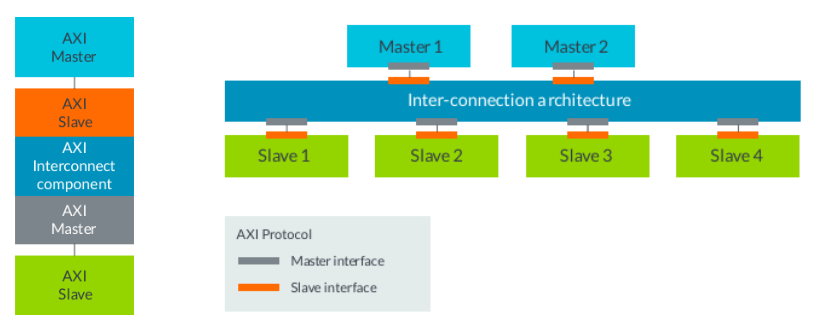
\includegraphics[width=1\linewidth]{chapter02/img/axi1.png}
    \caption{Sơ đồ AXI (AMBA)}
    \label{fig:placeholder}
\end{figure}

\subsection{Cơ sở lý thuyết và Cơ chế hoạt động của AXI4}
Giao thức AXI4 hoạt động dựa trên cơ chế ánh xạ bộ nhớ (Memory-Mapped I/O). Trong kiến trúc này, vi xử lý trung tâm không giao tiếp với các thiết bị ngoại vi thông qua các lệnh I/O đặc biệt, mà coi toàn bộ các khối phần cứng (Slave) như những dải địa chỉ bộ nhớ (Memory Addresses) liền kề \cite{arm_axi4_intro}.

\begin{figure}[!h]
    \centering
    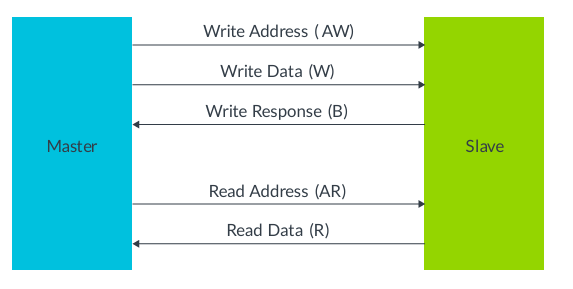
\includegraphics[width=1\linewidth]{chapter02/img/axi2.png}
    \caption{Các kênh giao tiếp (AMBA)}
    \label{fig:placeholder}
\end{figure}

Để đảm bảo hiệu suất truyền tải cao và hỗ trợ thực thi không theo thứ tự (Out-of-order execution), kiến trúc AXI4 phân tách các luồng dữ liệu thành 5 kênh (channels) độc lập, hoạt động song song và truyền theo một chiều duy nhất:
\begin{enumerate}
    \item \textbf{Kênh Địa chỉ Đọc (Read Address Channel - AR):} Truyền tải địa chỉ bắt đầu và các thông tin điều khiển cho quá trình đọc.
    \item \textbf{Kênh Dữ liệu Đọc (Read Data Channel - R):} Truyền dữ liệu từ Slave về Master, kèm theo cờ báo trạng thái đọc.
    \item \textbf{Kênh Địa chỉ Ghi (Write Address Channel - AW):} Truyền tải địa chỉ bắt đầu cho quá trình ghi dữ liệu.
    \item \textbf{Kênh Dữ liệu Ghi (Write Data Channel - W):} Truyền dữ liệu thực tế từ Master xuống Slave.
    \item \textbf{Kênh Phản hồi Ghi (Write Response Channel - B):} Slave phản hồi lại Master về trạng thái của toàn bộ giao dịch ghi (thành công hoặc có lỗi).
\end{enumerate}

\textbf{Cơ chế bắt tay:} 
Điểm cốt lõi làm nên độ tin cậy của AXI là cơ chế bắt tay hai chiều thông qua cặp tín hiệu \texttt{VALID} và \texttt{READY} có mặt trên tất cả 5 kênh. Master kéo tín hiệu \texttt{VALID} lên mức logic cao (1) để thông báo rằng dữ liệu hoặc địa chỉ trên bus đã hợp lệ. Ngược lại, Slave báo hiệu khả năng tiếp nhận bằng cách kéo tín hiệu \texttt{READY} lên cao. Một gói dữ liệu chỉ được coi là truyền thành công khi và chỉ khi cả \texttt{VALID} và \texttt{READY} đều ở mức 1 tại thời điểm sườn lên của xung nhịp (Clock Edge). Cơ chế này cho phép các khối phần cứng hoạt động ở các tần số xung nhịp khác nhau có thể đồng bộ hóa mà không gây ra hiện tượng mất mát dữ liệu hay thắt cổ chai (bottleneck).

\subsection{Phân loại các biến thể AXI trên nền tảng Xilinx}
Theo tài liệu \textit{Vitis Model Composer User Guide (UG1483)} của AMD/Xilinx \cite{ug1483}, giao thức AXI là tiêu chuẩn xương sống để đóng gói và kết nối các khối phần cứng. Tài liệu quy định quy trình ánh xạ (mapping) tự động các tín hiệu thuật toán cấp cao xuống ba biến thể AXI vật lý chính nhằm tối ưu hóa tài nguyên phần cứng và băng thông trên nền tảng FPGA:

\begin{itemize}
    \item \textbf{AXI4-Lite (Giao tiếp điều khiển vô hướng - Scalar):} 
    Theo UG1483, AXI4-Lite được sử dụng mặc định để ánh xạ các cổng tín hiệu đầu vào/đầu ra dạng vô hướng và các tín hiệu điều khiển (Control signals). Giao diện này tạo ra một bảng địa chỉ thanh ghi (Memory-Mapped Registers). Với đặc tính chỉ hỗ trợ truyền một đơn vị dữ liệu trong mỗi giao dịch (Single beat) và thiết kế logic cực kỳ nhỏ gọn, AXI4-Lite phù hợp để vi xử lý đọc/ghi trực tiếp vào các thanh ghi tĩnh của mạch gia tốc. Các thao tác điển hình bao gồm: ghi bit 1 để khởi động mạch (Start), đọc bit cờ báo hoàn thành (Done/Idle), hoặc nạp các tham số siêu tham số (Hyper-parameters) cho thuật toán.

    \item \textbf{AXI4 Memory-Mapped (AXI4-Full - Truy xuất khối tốc độ cao):} 
    Biến thể này được ứng dụng khi mô hình thiết kế cần giao tiếp với bộ nhớ đệm dùng chung dung lượng lớn như DDR RAM hoặc Block RAM (BRAM). Sức mạnh của AXI4-Full nằm ở khả năng truyền dữ liệu theo lô (Burst Transfer). CPU hoặc bộ điều khiển DMA (Direct Memory Access) chỉ cần cung cấp địa chỉ bắt đầu một lần duy nhất, sau đó có thể vận chuyển hàng ngàn byte dữ liệu (ví dụ: các bản đồ đặc trưng - Feature Maps của mạng CNN hoặc trọng số Weight) trong một chu kỳ thiết lập. Tính năng này giải quyết triệt để vấn đề "Bức tường bộ nhớ" (Memory Wall) trong các thiết kế gia tốc phần cứng AI.

    \item \textbf{AXI4-Stream (Dữ liệu luồng hướng sự kiện):} 
    Tài liệu chỉ định AXI4-Stream cho các luồng dữ liệu mảng (Array) tốc độ cực cao, phổ biến trong Xử lý tín hiệu số (DSP) và Xử lý ảnh (Vision AI). Khác biệt hoàn toàn với hai biến thể trên, AXI4-Stream truyền dữ liệu mà không cần địa chỉ bộ nhớ (Address-less). Nó hoạt động như một đường ống nước (Pipeline) kết nối trực tiếp đầu ra của khối này vào đầu vào của khối kia. Giao thức này chỉ sử dụng cơ chế bắt tay \texttt{TVALID} và \texttt{TREADY} để đẩy thông lượng (Throughput) lên mức tối đa mà không bị giới hạn bởi chu kỳ giải mã địa chỉ.
\end{itemize}

\subsection{Tích hợp hệ thống}

\textbf{Quy trình đóng gói phần cứng (IP Packaging):}
Một điểm nhấn quan trọng trong hệ sinh thái thiết kế của Xilinx (UG1483) là khả năng tự động hóa việc đóng gói. Khi thiết kế lõi thuật toán bằng ngôn ngữ mô tả phần cứng (Verilog/SystemVerilog), công cụ IP Packager không chỉ tổng hợp mạch logic lõi mà còn tự động sinh ra lớp bọc (wrapper) chứa các giao diện AXI chuẩn mực. Đồng thời, hệ thống cũng tự động khởi tạo bộ thư viện trình điều khiển phần mềm (C/C++ Driver API / BSP). Điều này cho phép hệ điều hành hoặc mã Bare-metal dễ dàng tương tác với khối phần cứng thông qua các hàm truy xuất thanh ghi tiêu chuẩn trong môi trường Vitis thống nhất.

\textbf{Ứng dụng chuẩn AXI vào Kiến trúc Gia tốc Mạng nơ-ron:}
Dựa trên nền tảng lý thuyết của giao thức AXI, kiến trúc của đồ án được định hình xoay quanh việc triển khai hệ thống nhận diện vật thể ứng dụng mô hình CNN lượng tử hóa (INT8) trên SoC Zynq UltraScale+ (Kit phát triển Kria KV260). Hệ thống là sự kết hợp đồng bộ giữa phần mềm chạy trên tập lệnh RISC-V (lõi mềm CV32E40P) và phần cứng gia tốc logic (CNN Accelerator). Giao thức AXI đóng vai trò cốt lõi trong việc định tuyến toàn bộ luồng điều khiển và luồng dữ liệu của thiết kế:

\begin{itemize}
    \item \textbf{Luồng Điều khiển (Control Flow) với AXI4-Lite:} Khối gia tốc phần cứng được tích hợp cổng giao tiếp Slave AXI4-Lite, được ánh xạ vào một dải địa chỉ cơ sở tĩnh trên không gian bộ nhớ của hệ thống (Memory-mapped). Vi xử lý trung tâm sử dụng đường truyền này để can thiệp trực tiếp vào máy trạng thái (FSM) của khối CNN. Cụ thể, các lệnh ghi/đọc được sử dụng để kích hoạt cờ vận hành (Start), hoặc kiểm tra trạng thái hoạt động (Status/Done). Để tối ưu hóa thời gian tính toán song song, hệ thống được thiết kế kết hợp phát tín hiệu ngắt cứng (IRQ) qua bộ điều khiển ngắt, giải phóng CPU khỏi việc phải liên tục chờ đợi vòng lặp (Polling).
    
    \item \textbf{Luồng Dữ liệu (Data Flow) với Kiến trúc Bộ nhớ dùng chung (Shared Memory):} Để giải quyết bài toán thắt cổ chai dữ liệu khi cả lõi RISC-V và lõi gia tốc CNN cùng cần truy xuất thông tin, hệ thống sử dụng một khối Block RAM (BRAM) cấu hình cổng kép (True Dual-Port BRAM) làm vùng nhớ dùng chung. Giao diện AXI4 kết nối vùng vi xử lý Host (nhân Cortex-A) và lõi RISC-V vào hệ thống BRAM này. Ban đầu, vi xử lý Host đóng vai trò quản lý tài nguyên, thực hiện nạp firmware cho RISC-V và đưa dữ liệu ảnh đầu vào (Inference Data) xuống BRAM thông qua bus AXI. Sau khi giải phóng tín hiệu Reset, lõi RISC-V sẽ trực tiếp nạp lệnh từ BRAM và đóng vai trò điều khiển độc lập để chỉ đạo khối CNN tính toán.
\end{itemize}

Việc tuân thủ chặt chẽ tiêu chuẩn giao tiếp AMBA AXI trong thiết kế này không chỉ đảm bảo hệ thống vận hành ổn định trên nền tảng FPGA Kria KV260, mà còn mang ý nghĩa lớn về mặt kiến trúc. Nền tảng Zynq hiện tại đóng vai trò là môi trường ASIC Prototyping. Khi định hướng đưa hệ thống vi mạch Edge AI này vào sản xuất thực tế (Tape-out), toàn bộ lõi RISC-V và bộ gia tốc CNN chuẩn AXI có thể được tái sử dụng trực tiếp trên đế Silicon (ASIC) mà không cần phải tái cấu trúc giao thức giao tiếp, khẳng định tính chuyên nghiệp và định hướng công nghiệp của đồ án.
%=================================================
%
%=================================================
\newpage
\section{tổng quan về trí tuệ nhân tạo (ai)}
\label{sec:ai_overview}

\subsection{Các Mô hình AI (AI Models)}
Trong lĩnh vực thị giác máy tính và hệ thống nhúng, các mô hình AI thường được phân loại dựa trên chức năng và kiến trúc. Việc lựa chọn mô hình phù hợp là yếu tố quyết định đến hiệu năng của hệ thống Edge AI.

\subsubsection{Mô hình Phân loại (Classification)}
Đây là dạng mô hình cơ bản nhất, nhiệm vụ là gán nhãn cho một hình ảnh đầu vào. Ví dụ: xác định xem trong ảnh có người hay không. Các kiến trúc tiêu biểu bao gồm MobileNet, SqueezeNet, và ResNet. Đối với các thiết bị biên, MobileNet thường được ưu tiên nhờ kiến trúc Depthwise Separable Convolution giúp giảm đáng kể khối lượng tính toán.

\subsubsection{Mô hình Phát hiện đối tượng (Object Detection)}
Phức tạp hơn phân loại, mô hình này không chỉ xác định đối tượng là gì mà còn định vị vị trí của nó thông qua các khung bao (Bounding Box). Các đại diện nổi bật gồm dòng YOLO (You Only Look Once) và SSD (Single Shot MultiBox Detector). Tuy nhiên, việc triển khai Object Detection trên soft-core RISC-V đòi hỏi tài nguyên tính toán rất lớn.

\subsubsection{Mô hình Phân đoạn (Segmentation)}
Phân loại từng pixel trong ảnh, giúp tách nền và đối tượng một cách chi tiết. Dạng mô hình này (ví dụ: U-Net) thường yêu cầu bộ nhớ lớn để lưu trữ các bản đồ đặc trưng (feature maps) độ phân giải cao, do đó ít được ưu tiên trên các hệ thống FPGA tài nguyên thấp nếu không có bộ tăng tốc phần cứng chuyên dụng.

\subsection{Training và Inference}
Để triển khai AI trên phần cứng, cần phân biệt rõ hai giai đoạn:
\begin{itemize}
    \item \textbf{Huấn luyện (Training):} Quá trình tìm ra bộ trọng số (weights) tối ưu cho mô hình thông qua việc học từ dữ liệu lớn. Quá trình này yêu cầu tính toán dấu phẩy động (Float32/Float16) và thường thực hiện trên Server hoặc GPU mạnh.
    \item \textbf{Suy luận (Inference):} Quá trình sử dụng mô hình đã huấn luyện để đưa ra dự đoán trên dữ liệu mới. Tại thiết bị biên (Edge), suy luận yêu cầu độ trễ thấp và thường sử dụng kỹ thuật lượng tử hóa để chạy trên phần cứng số nguyên (Integer hardware) như RISC-V soft-core.
\end{itemize}

\subsection{Phân loại AI và Mối liên hệ với Deep Learning}
Trí tuệ nhân tạo là một thuật ngữ rộng, bao hàm nhiều cấp độ:
\begin{itemize}
    \item \textbf{AI hẹp (Narrow AI):} Các hệ thống được thiết kế cho một tác vụ cụ thể (như nhận dạng ảnh trong đề tài này).
    \item \textbf{Học máy (Machine Learning - ML):} Tập con của AI, nơi máy tính học từ dữ liệu thay vì được lập trình quy tắc cứng.
    \item \textbf{Học sâu (Deep Learning - DL):} Tập con của ML, sử dụng các mạng nơ-ron nhiều lớp để trích xuất đặc trưng tự động.
\end{itemize}
\textit{Chi tiết về cấu trúc và nguyên lý hoạt động của Mạng nơ-ron nhân tạo (ANN) và Học sâu sẽ được trình bày chuyên sâu tại Mục \ref{sec:neural_network}.}

\subsection{Edge AI}

\subsubsection{Khái niệm}
Edge AI là sự kết hợp giữa thuật toán AI và tính toán biên (Edge Computing), cho phép xử lý dữ liệu cục bộ ngay trên thiết bị phần cứng mà không cần gửi dữ liệu về trung tâm dữ liệu (Cloud).

\subsubsection{Ưu điểm so với Cloud AI}
\begin{itemize}
    \item \textbf{Độ trễ thấp (Low Latency):} Phản hồi tức thời, phù hợp cho các ứng dụng thời gian thực (ví dụ: xe tự lái, robot).
    \item \textbf{Bảo mật và Quyền riêng tư:} Dữ liệu hình ảnh nhạy cảm không rời khỏi thiết bị, giảm nguy cơ bị tấn công đường truyền.
    \item \textbf{Tiết kiệm băng thông:} Không cần truyền tải luồng video liên tục lên máy chủ, giảm tải cho hạ tầng mạng.
    \item \textbf{Độ tin cậy:} Hệ thống vẫn hoạt động bình thường ngay cả khi mất kết nối Internet.
\end{itemize}

\subsubsection{Các Framework phổ biến cho Edge AI}
\begin{itemize}
    \item \textbf{TensorFlow Lite (TFLite):} Phiên bản rút gọn của TensorFlow, tối ưu cho thiết bị di động và nhúng. TFLite hỗ trợ chuyển đổi mô hình sang định dạng FlatBuffer nhẹ và cung cấp các toán tử tối ưu cho vi xử lý ARM và RISC-V.
    \item \textbf{Vitis AI:} Nền tảng phát triển của AMD-Xilinx, chuyên dụng để tối ưu hóa mô hình AI chạy trên các kiến trúc DPU (Deep Learning Processor Unit) của FPGA Xilinx.
    \item \textbf{ONNX Runtime:} ONNX (Open Neural Network Exchange) là định dạng trung gian giúp chuyển đổi mô hình giữa các framework (PyTorch sang TensorFlow). ONNX Runtime cho phép chạy suy luận hiệu năng cao trên nhiều nền tảng phần cứng khác nhau.
\end{itemize}

%=================================================
%=================================================
\section{Mạng Nơ-ron Nhân tạo (Artificial Neural Networks)}
\label{sec:neural_network}

Mạng nơ-ron nhân tạo (ANN) là nền tảng của Deep Learning, 
lấy cảm hứng từ cơ chế truyền dẫn tín hiệu điện hóa giữa các nơ-ron 
trong bộ não sinh học. Trước khi đi sâu vào kiến trúc CNN được sử dụng trong đề tài, 
cần xem xét tổng quan các kiến trúc mạng nơ-ron phổ biến để thấy rõ sự phù hợp 
của từng loại đối với các tác vụ cụ thể.\cite{CNN}

\subsection{Các kiến trúc Mạng Nơ-ron phổ biến}

\subsubsection{Mạng Nơ-ron Truyền thẳng (Feedforward Neural Network - MLP)}
Đây là dạng đơn giản nhất của ANN, còn được gọi là Multi-Layer Perceptron (MLP). Trong kiến trúc này, thông tin di chuyển theo một chiều từ lớp đầu vào (Input), qua các lớp ẩn (Hidden layers) đến lớp đầu ra (Output) mà không có chu trình quay lại.
\begin{itemize}
    \item \textbf{Đặc điểm:} Các nơ-ron ở lớp trước kết nối đầy đủ (fully connected) với nơ-ron lớp sau.
    \item \textbf{Hạn chế với hình ảnh:} Khi xử lý ảnh, MLP làm mất thông tin không gian (spatial structure) do phải duỗi phẳng ảnh thành vector 1 chiều. Ngoài ra, số lượng tham số bùng nổ quá nhanh dẫn đến quá tải bộ nhớ và hiện tượng quá khớp (overfitting).
\end{itemize}

\subsubsection{Các kiến trúc khác}
Ngoài MLP, lĩnh vực mạng nơ-ron còn có Mạng nơ-ron Hồi quy (RNN, với các biến thể LSTM/GRU) chuyên cho dữ liệu chuỗi thời gian, và Vision Transformers (ViT) áp dụng cơ chế Self-Attention. Tuy nhiên, RNN không hiệu quả trong việc trích xuất đặc trưng không gian 2D và khó song song hóa, còn ViT có độ phức tạp $O(N^2)$ tiêu tốn tài nguyên rất lớn -- cả hai đều không phù hợp với ràng buộc của một soft-core RISC-V trên FPGA tài nguyên hạn chế. Do đó, đồ án lựa chọn Mạng nơ-ron Tích chập (CNN) làm kiến trúc chính, sẽ được trình bày tại mục~\ref{sec:cnn}.

\subsection{Mạng Nơ-ron Tích chập (CNN)}
\label{sec:cnn}
Dựa trên phân tích trên, CNN là kiến trúc cân bằng nhất giữa hiệu năng và chi phí tính toán cho các thiết bị biên. CNN là kiến trúc mạng chuyên biệt cho dữ liệu dạng lưới (grid-like topology) như hình ảnh. Một mạng CNN điển hình bao gồm ba loại lớp chính:

\subsubsection{Lớp Tích chập (Convolutional Layer)}

Đây là lớp quan trọng nhất, thực hiện trích xuất đặc trưng cục bộ và bảo toàn tính chất không gian của ảnh. Phép tính tích chập là việc trượt một cửa sổ nhỏ (Kernel/Filter) trên toàn bộ ảnh đầu vào và thực hiện phép nhân chập.
Về mặt toán học, giá trị đầu ra $Y$ tại vị trí $(i, j)$ được tính như sau:
\begin{equation}
Y[i, j] = \sum_{m} \sum_{n} X[i+m, j+n] \cdot K[m, n] + b
\end{equation}
Trong đó: $X$ là ma trận đầu vào, $K$ là ma trận Kernel, và $b$ là bias. Trên các vi xử lý RISC-V hỗ trợ DSP (như Pulpino), phép toán này có thể được tăng tốc bằng các lệnh SIMD (Single Instruction Multiple Data), cho phép thực hiện 4 phép nhân 8-bit trong một chu kỳ xung nhịp.

\subsubsection{Hàm kích hoạt (Activation Function)}
Hàm kích hoạt giúp đưa tính phi tuyến vào mô hình, cho phép mạng học được các đặc trưng phức tạp. Hàm phổ biến nhất trong CNN là \textbf{ReLU (Rectified Linear Unit)}:
\begin{equation}
f(x) = \max(0, x)
\end{equation}
ReLU có ưu điểm lớn về mặt tính toán trên phần cứng nhúng vì chỉ cần một lệnh so sánh đơn giản (nếu $x < 0$ thì gán bằng 0), không tốn kém tài nguyên như hàm Sigmoid hay Tanh (vốn yêu cầu tính toán số mũ thực rất nặng nề cho soft-core).

\subsubsection{Lớp Gộp (Pooling Layer)}
Dùng để giảm kích thước không gian của bản đồ đặc trưng (down-sampling), giúp giảm số lượng tham số và tính toán, đồng thời giúp mô hình bất biến với các dịch chuyển nhỏ (Translation Invariance) của đối tượng. Hai kỹ thuật phổ biến là Max Pooling (lấy giá trị lớn nhất) và Average Pooling (lấy giá trị trung bình).

\subsection{Kỹ thuật Lượng tử hóa (Quantization)}
Lượng tử hóa là kỹ thuật cốt lõi để triển khai AI trên các vi xử lý RISC-V soft-core không có bộ xử lý dấu phẩy động (FPU) mạnh mẽ.

\subsubsection{Khái niệm}
Kỹ thuật này chuyển đổi các trọng số (weights) và giá trị kích hoạt (activations) từ dạng số thực 32-bit (Float32) sang số nguyên 8-bit (Int8). Công thức chuyển đổi tổng quát:
\begin{equation}
r = S \times (q - Z)
\end{equation}
Trong đó: $r$ là giá trị thực, $q$ là giá trị lượng tử hóa (int8), $S$ là tỉ lệ (Scale factor), và $Z$ là điểm không (Zero-point).

\subsubsection{Lợi ích trên FPGA/RISC-V}
\begin{itemize}
    \item \textbf{Giảm bộ nhớ:} Kích thước mô hình giảm 4 lần (từ 32-bit xuống 8-bit), giúp mô hình vừa vặn với bộ nhớ on-chip (BRAM/TCM) hạn hẹp của FPGA, giảm độ trễ truy cập bộ nhớ ngoài (DDR).
    \item \textbf{Tăng tốc độ:} Các phép tính số học trên số nguyên (Integer Arithmetic) nhanh hơn và tiêu thụ ít năng lượng hơn nhiều so với số thực. Các nhân RISC-V như RI5CY hỗ trợ thực hiện 4 phép nhân cộng Int8 trong một chu kỳ máy.
\end{itemize}

\subsection{Các kỹ thuật tối ưu hóa khác}

\subsubsection{Kỹ thuật Cắt tỉa }
Pruning loại bỏ các kết nối (trọng số) có giá trị gần bằng 0 hoặc ít ảnh hưởng đến kết quả đầu ra. Kỹ thuật này biến ma trận trọng số dày đặc (Dense) thành ma trận thưa (Sparse), giúp giảm đáng kể khối lượng tính toán và bộ nhớ lưu trữ mà không làm giảm nhiều độ chính xác.

\subsubsection{Kỹ thuật im2col (Image-to-Column)}

Để tối ưu hóa phép tính tích chập trên phần cứng, kỹ thuật \textit{im2col} thường được sử dụng. Nó biến đổi ma trận ảnh đầu vào thành các cột, chuyển bài toán tích chập phức tạp (Convolution) thành bài toán nhân ma trận (GEMM - General Matrix Multiply). GEMM là phép toán đã được tối ưu hóa rất tốt trên các thư viện tính toán (như BLAS) và tận dụng triệt để khả năng xử lý song song.

Trong đồ án này, bộ tăng tốc Conv-CNN v2.0 không sử dụng \textit{im2col} vì áp dụng kiến trúc \textit{streaming dataflow} với line buffer + window register: dữ liệu được trượt qua window $3 \times 3$ và đưa vào trực tiếp 9 PE MAC, tránh chi phí biến đổi và sao chép bộ nhớ của \textit{im2col}.

\chapter {Các công trình nghiên cứu liên quan}
\label{chp:03}

Chương này trình bày các công trình tiêu biểu trong ba hướng nghiên cứu liên quan đến đề tài: (i) các vi xử lý mã nguồn mở dựa trên RISC-V cho ứng dụng Edge AI, (ii) các framework gia tốc CNN trên FPGA, và (iii) các kiến trúc mạng nơ-ron và kỹ thuật lượng tử hóa hiệu quả cho thiết bị biên. Phần kết của mỗi mục sẽ làm rõ vị trí thiết kế của đề tài so với từng hướng tiếp cận đã có.

%=================================================================================
\section{Vi xử lý mã nguồn mở RISC-V cho Edge AI}
\label{sec:riscv_related}

\subsection{Hệ sinh thái PULP và Pulpissimo}
PULPissimo (PULP Independent Single-stream Shared-memory Integrated Subsystem) là một SoC vi điều khiển 32-bit dựa trên RISC-V, được phát triển bởi nhóm PULP (Parallel Ultra Low Power) thuộc ETH Zürich và Đại học Bologna \cite{pulpissimo}. Pulpissimo cung cấp một nền tảng phần cứng tiết kiệm năng lượng nhưng vẫn đảm bảo hiệu năng tính toán cho IoT và Edge AI, bao gồm: lõi RI5CY (tên cũ của CV32E40P), hệ thống bộ nhớ TCDM 16-bank, bộ điều khiển uDMA cho ngoại vi, hệ thống ngắt, và giao diện Hardware Processing Engine (HWPE) cho các bộ tăng tốc tùy chỉnh.

Đề tài này \textbf{kế thừa lõi xử lý CV32E40P từ Pulpissimo} (qua submodule chính thức của OpenHW Group) nhưng \textbf{không sử dụng các thành phần khác} của Pulpissimo: thay vì TCDM 16-bank + Logarithmic Interconnect, đề tài thiết kế lại memory subsystem theo chuẩn AXI4 của Xilinx (dual-port BRAM + AXI SmartConnect). Lựa chọn này nhằm tích hợp tự nhiên với Vivado IP Catalog và đồng bộ địa chỉ logic giữa ARM và RISC-V (xem mục~\ref{sec:pl_design}).

\subsection{Mở rộng tập lệnh RISC-V cho mạng nơ-ron}
Một hướng tiếp cận để gia tốc mạng nơ-ron trên RISC-V là can thiệp trực tiếp vào kiến trúc tập lệnh (ISA Extensions). Công trình \textit{``FPGA-Accelerated RISC-V ISA Extensions for Efficient Neural Network Inference on Edge Devices''} \cite{parameshwara2025fpga} là một minh chứng tiêu biểu cho trường phái thiết kế \textit{tightly-coupled}: thay vì tách bộ tăng tốc thành IP độc lập, nhóm tác giả định nghĩa các chỉ thị MAC INT8 mới, tích hợp ngay vào pipeline ALU của lõi RISC-V.

\textbf{Ưu điểm} của hướng này là độ trễ giao tiếp gần như bằng 0 (không qua bus AXI) và tiết kiệm năng lượng do không phải đọc/ghi bộ nhớ ngoài. \textbf{Nhược điểm}: (i) đòi hỏi can thiệp sâu vào RTL của CPU, có rủi ro làm giảm Fmax; (ii) bị giới hạn bởi băng thông tập thanh ghi 32-bit, khó scale lên các layer lớn; (iii) cần custom GCC/LLVM toolchain để biên dịch các lệnh tùy biến.

\textbf{Đối chiếu với đề tài:} Đề tài chọn hướng \textit{loosely-coupled} (Conv-CNN là IP độc lập giao tiếp qua AXI), đánh đổi độ trễ giao tiếp lấy tính module hóa và khả năng scale. Lõi RISC-V CV32E40P được giữ nguyên bản (RV32IMC standard), không cần custom toolchain -- ưu tiên tính bảo trì và tái sử dụng cho các capstone project sau.

%=================================================================================
\newpage
\section{Framework gia tốc CNN trên FPGA}
\label{sec:fpga_frameworks}

Phần này tổng hợp 4 framework tiêu biểu cho việc gia tốc CNN trên FPGA, được lựa chọn dựa trên mức độ phù hợp với platform của đề tài (Xilinx Zynq UltraScale+) và tính đại diện cho các trường phái thiết kế khác nhau.

\subsection{Vitis AI DPU (Xilinx)}
Vitis AI Deep Processing Unit (DPU) là giải pháp thương mại của Xilinx (nay là AMD-Xilinx) dành cho việc triển khai CNN trên dòng SoC Zynq UltraScale+ (bao gồm Kria KV260) \cite{vitis_ai}. DPU được phân phối dưới dạng IP đóng (encrypted bitstream), kèm theo compiler chuyển mô hình từ TensorFlow/PyTorch sang chỉ thị máy của DPU. Người dùng chỉ cần quantize mô hình và gọi runtime API, không cần thiết kế RTL.

\textbf{Đối chiếu với đề tài:} DPU cho phép triển khai nhanh nhiều mô hình lớn (ResNet, MobileNet, YOLO) nhưng có ba hạn chế đáng kể: (i) \textit{closed-source} -- không thể tùy biến op set hay quantization scheme; (ii) tài nguyên cố định -- DPU B1024/B2048 chiếm phần lớn FPGA, khó nhường chỗ cho RISC-V soft-core; (iii) không có khả năng \textit{hardware-software co-design} ở mức RTL -- yếu tố cốt lõi của đề tài. Đề tài chấp nhận phạm vi op nhỏ hơn nhưng đổi lấy tính kiểm soát hoàn toàn pipeline phần cứng.

\subsection{FINN -- HLS-based BNN Accelerator (Xilinx Research)}
FINN \cite{finn_paper} là framework do Xilinx Research phát triển, sinh tự động bộ tăng tốc cho Binarized Neural Networks (BNN, weights/activations 1-bit) qua Vivado HLS. FINN tận dụng đặc điểm BNN -- thay phép tích chập bằng XNOR + Popcount thực hiện hoàn toàn bằng LUT -- để đạt throughput cao mà không tốn DSP.

\textbf{Đối chiếu với đề tài:} BNN cho phép throughput cực cao (hàng nghìn img/s) nhưng giảm độ chính xác đáng kể trên các tập dữ liệu phức tạp. Đề tài chọn INT8 (đề xuất bởi Jacob et al. \cite{jacob2018quantization}) làm điểm cân bằng tốt hơn giữa chính xác và hiệu năng cho bài toán phân loại nhị phân, đồng thời tận dụng được DSP48E2 của Ultrascale+ (vốn dồi dào: 1248 DSP trên KV260).

\subsection{hls4ml (CERN -- Fermilab Collaboration)}
hls4ml \cite{hls4ml} là framework do nhóm vật lý hạt nhân (CERN, Fermilab) phát triển ban đầu cho ứng dụng trigger LHC, nay được mở rộng cho Edge AI. hls4ml nhận mô hình Keras/PyTorch làm đầu vào và sinh ra C++ HLS code, sau đó qua Vivado HLS để tổng hợp thành RTL. Toàn bộ mạng được \textit{fully unrolled} thành dataflow pipeline, đạt độ trễ rất thấp (microsecond range).

\textbf{Đối chiếu với đề tài:} hls4ml hoàn toàn HLS-based, không có CPU tham gia điều phối -- mô hình bị ``cứng hóa'' thành RTL, đổi mô hình phải re-synthesize bitstream. Đề tài giữ kiến trúc phân tầng với RISC-V làm orchestrator: đổi mô hình chỉ cần thay \texttt{layer\_table.h} + \texttt{weights.bin}, không cần re-synth -- phù hợp hơn với mục tiêu prototyping nhanh nhiều mô hình.

\subsection{CFU Playground (Google)}
CFU Playground \cite{cfu_playground} là project mã nguồn mở của Google, kết hợp lõi RISC-V (VexRiscv) với Custom Function Unit (CFU) trên FPGA, chạy TensorFlow Lite Micro. CFU là một dạng \textit{tightly-coupled} accelerator: được thêm vào ALU của RISC-V qua chỉ thị tùy biến, gần giống hướng tiếp cận của \cite{parameshwara2025fpga}.

\textbf{Đối chiếu với đề tài:} CFU Playground và đề tài đại diện cho hai trường phái song song trong nghiên cứu RISC-V + AI:
\begin{itemize}
    \item \textbf{CFU Playground (tightly-coupled):} Bộ tăng tốc nằm trong lõi CPU, chia sẻ register file. Phù hợp khi mô hình nhỏ và op đơn giản (thường ở mức MAC vector).
    \item \textbf{Đề tài (loosely-coupled):} Bộ tăng tốc là IP độc lập giao tiếp qua AXI và DMA. Phù hợp khi op phức tạp (Conv 3$\times$3 với line buffer + window + requantize) và cần streaming bandwidth cao từ DDR.
\end{itemize}
Lựa chọn của đề tài nghiêng theo hướng loosely-coupled vì: (i) op chính là Conv 3$\times$3 với line buffer 16~KB BRAM -- không thể nhét vào trong CPU; (ii) cần DMA tốc độ cao từ DDR mà CFU không hỗ trợ trực tiếp.

\subsection{Bảng tổng hợp so sánh}
\begin{table}[!h]
    \centering
    \caption{So sánh đa chiều các framework gia tốc CNN trên FPGA.}
    \label{tab:framework_comparison}
    \resizebox{\textwidth}{!}{%
    \begin{tabular}{|l|c|c|c|c|c|}
    \hline
    \textbf{Framework} & \textbf{Mã nguồn} & \textbf{Coupling} & \textbf{Quantization} & \textbf{Đổi mô hình} & \textbf{Có RISC-V?} \\ \hline
    Vitis AI DPU       & Closed   & Loosely (DPU IP)        & INT8           & Compile lại model    & Không (chỉ ARM) \\ \hline
    FINN               & Open     & Loosely (HLS-gen IP)    & 1-bit (BNN)    & Re-synthesize        & Không           \\ \hline
    hls4ml             & Open     & N/A (fully unrolled)    & FP/INT tùy chọn & Re-synthesize       & Không           \\ \hline
    CFU Playground     & Open     & Tightly (in-CPU)        & INT8 (TFLM)    & Re-compile firmware  & Có (VexRiscv)   \\ \hline
    \textbf{Đề tài}    & Open     & Loosely (AXI IP)        & INT8 (TFLite)  & Thay weights+table   & Có (CV32E40P)   \\ \hline
    \end{tabular}%
    }
\end{table}

%=================================================================================
\newpage
\section{Mô hình hiệu quả cho thiết bị biên}
\label{sec:efficient_models}

Bên cạnh các vi xử lý mở và framework FPGA, hướng nghiên cứu thứ ba để đưa AI lên thiết bị biên là tối ưu hóa kiến trúc mạng nơ-ron thay vì phần cứng. Hai trường phái tiêu biểu được tóm tắt dưới đây để làm rõ vị trí thiết kế của đề tài.

\paragraph{Mạng nơ-ron Nhị phân (BNN).} Courbariaux và cộng sự \cite{bnn_courbariaux} đã chứng minh khả năng huấn luyện các mạng nơ-ron sâu với trọng số và kích hoạt ép buộc về $\{+1, -1\}$ (1-bit). Lợi thế lớn nhất của BNN trên FPGA là phép tích chập được thay bằng phép logic XNOR + Popcount, có thể thực hiện trực tiếp bằng LUT mà không cần DSP. Tuy nhiên, BNN gặp giảm độ chính xác đáng kể trên các tập dữ liệu phức tạp (ImageNet). Đồ án tham khảo nguyên lý tối ưu phần cứng của BNN nhưng lựa chọn lượng tử hóa INT8 chuẩn TFLite \cite{jacob2018quantization} để đạt cân bằng tốt hơn giữa độ chính xác và hiệu năng.

\paragraph{MobileNet và Depthwise Separable Convolution.} Howard và cộng sự \cite{mobilenet_v1} đề xuất kiến trúc MobileNet sử dụng \textit{depthwise separable convolution} (tách Conv $K \times K$ thành Depthwise Conv + Pointwise $1 \times 1$) để giảm khoảng 8--9 lần số phép MAC so với Conv chuẩn cùng kích thước. MobileNet trở thành kiến trúc chuẩn cho thị giác máy trên thiết bị di động. Tuy nhiên, depthwise convolution có \textit{dataflow ngược} so với Conv chuẩn (mỗi cin $\to$ 1 output thay vì sum across cin), đòi hỏi MUX adder tree riêng và chế độ FSM mới ở bộ tăng tốc. Trong phạm vi đồ án, đề tài chọn kiến trúc \texttt{vgg-tiny} đơn giản hơn (chỉ Conv $3 \times 3$ chuẩn) để tập trung vào việc kiểm chứng đồng thiết kế phần cứng-phần mềm; hỗ trợ depthwise được dành cho hướng phát triển tiếp theo.

%=================================================================================
\section{Lượng tử hóa và huấn luyện mạng nơ-ron}
\label{sec:quantization_theory}

Trong các hệ thống học sâu truyền thống, việc huấn luyện và suy luận thường được
thực hiện trên định dạng số thực dấu phẩy động 32-bit (Float32) để đảm bảo độ chính xác cao nhất. Tuy nhiên, trên các thiết bị biên (Edge Devices) với tài nguyên hạn chế như FPGA hay vi xử lý nhúng RISC-V, các phép toán số thực tiêu tốn quá nhiều tài nguyên phần cứng và năng lượng.

Để giải quyết vấn đề này, đồ án áp dụng phương pháp lượng tử hóa số nguyên
được đề xuất bởi \textit{Jacob et al.} (Google) trong công trình
\textit{"Quantization and Training of Neural Networks for Efficient
Integer-Arithmetic-Only Inference"} \cite{jacob2018quantization}.

\begin{figure}[!h]
    \centering
    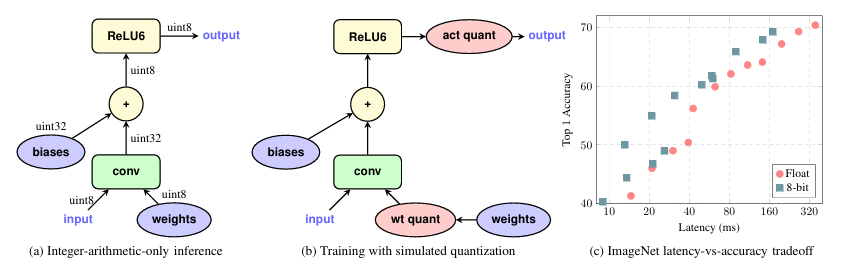
\includegraphics[width=1\linewidth]{chapter03/img/quanti.png}
    \caption{Quy trình lượng tử hóa và huấn luyện mạng nơ-ron theo Jacob et al.}
    \label{fig:quantization_process}
\end{figure}

\subsection{Cơ chế Lượng tử hóa Affine (Affine Quantization Scheme)}
Khác với các phương pháp lượng tử hóa logarit hay nhị phân, phương pháp của Jacob et al. sử dụng ánh xạ tuyến tính (Affine mapping) để chuyển đổi giữa giá trị thực ($r$) và giá trị nguyên 8-bit ($q$). Công thức ánh xạ được định nghĩa như sau:

\begin{equation}
    r = S \times (q - Z)
\end{equation}

Trong đó:
\begin{itemize}
    \item $r$ (Real value): Giá trị thực cần biểu diễn.
    \item $q$ (Quantized value): Giá trị nguyên 8-bit ($q \in [0, 255]$ hoặc $[-128, 127]$).
    \item $S$ (Scale factor): Hằng số tỉ lệ (dạng Float32 dương), xác định bước nhảy của lượng tử hóa.
    \item $Z$ (Zero-point): Giá trị nguyên đóng vai trò là điểm "0" của số thực. Điều này cho phép biểu diễn chính xác giá trị 0 thực tế (thường xuất hiện trong Padding hoặc ReLU) bằng một số nguyên, giúp duy trì độ chính xác của mạng.
\end{itemize}

Từ công thức trên, quá trình nhân chập (Convolution) giữa đầu vào $x$ và trọng số $w$ có thể được viết lại hoàn toàn dưới dạng số nguyên:

\begin{equation}
    y = \sum (x \times w) \approx S_y \left( \sum (q_x - Z_x)(q_w - Z_w) + Z_y \right)
\end{equation}

\subsection{Suy luận chỉ dùng số học nguyên (Integer-Arithmetic-Only Inference)}
Điểm đột phá trong nghiên cứu của Jacob et al. là kỹ thuật xử lý tham số $S$ (Scale). Mặc dù $S$ là số thực, nhưng trong quá trình suy luận, tích của các Scale ($M = S_x S_w / S_y$) được xấp xỉ bằng một phép nhân số nguyên và phép dịch bit (Bit-shift):

\begin{equation}
    M \approx 2^{-n} \times M_0 \quad (\text{với } M_0 \text{ là số nguyên cố định})
\end{equation}

Kỹ thuật này cho phép loại bỏ hoàn toàn khối xử lý số thực (FPU) khỏi phần cứng.
Mọi phép tính từ tích chập, cộng bias đến hàm kích hoạt đều được thực hiện bằng
các đơn vị số học nguyên (ALU Integer) và các bộ dịch bit. Đề tài hiện thực trực tiếp công thức này trong module \texttt{requantize.sv} với pipeline 3-tầng (mục~\ref{ssec:requantize}).

\chapter{Thiết kế kiến trúc hệ thống}
\label{chp:04}

\section{Tổng quan kiến trúc Platform}

Để đảm bảo tính linh hoạt, khả năng mở rộng và tái sử dụng, hệ thống được thiết kế dựa trên mô hình phân lớp chức năng. Kiến trúc này cho phép tách biệt giữa hạ tầng phần cứng vật lý và logic thực thi của ứng dụng AI.

\begin{figure}[!h]
\centering
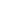
\includegraphics[width=0.6\textwidth]{chapter04/img/platform.png}
\caption{Stack kiến trúc hệ thống Edge-AI}
\end{figure}

\begin{itemize}
    \item Lớp 1: Hardware Layer (Cơ sở hạ tầng)Phân tích lý do chọn Zynq 
    làm Host (Quản lý I/O tốt, chạy Linux) và CV32E40P làm Accelerator 
    (Lõi nhỏ gọn, hỗ trợ tập lệnh IMC, tối ưu diện tích chip)
    .Nhấn mạnh vào khối AXI Interconnect và BRAM Controller 
    (Phiên dịch viên ngôn ngữ bus) - Đây chính là xương sống của Platform.
    \item Lớp 2: Software / Runtime Layer (Hệ điều hành \& Trình điều khiển)
    Trình bày luồng hoạt động (Data Flow): ARM đóng vai trò Master, 
    dùng Memory Mapped I/O để đẩy dữ liệu. RISC-V đóng vai trò Slave, 
    luôn ở trạng thái chờ lệnh (Polling)
    ARM chụp ảnh $\rightarrow$
    Đẩy vào BRAM $\rightarrow$ Kích hoạt cờ (Flag) $\rightarrow$ 
    RISC-V đọc cờ $\rightarrow$ Tính toán $\rightarrow$ Ghi kết quả 
    $\rightarrow$ ARM đọc kết quả.
    \item Lớp 3: Application Layer (Tầng ứng dụng): Một 
    nền tảng "mở". Hiện tại đang chạy nhận diện người (CNN), nhưng vì 
    là Platform, ngày mai người dùng hoàn toàn có thể nạp firmware 
    khác để chạy nhận diện âm thanh mà không cần sửa lại phần cứng.
\end{itemize}


\subsection{Layer 1: Hardware Layer}
Đây là tầng thấp nhất của nền tảng, thực thi các tác vụ tính toán cường độ cao và quản lý luồng dữ liệu thô. Thành phần chính bao gồm:

Hệ thống xử lý (Processing System - PS): Tận dụng cụm lõi ARM Cortex-A53 của Zynq UltraScale+ để điều phối toàn hệ thống.

Bộ gia tốc lõi mềm (Soft-core Accelerator): Lõi vi xử lý RISC-V CV32E40P kết hợp cùng khối tăng tốc phần cứng (CNN Accelerator) tùy chỉnh trên vùng Programmable Logic (PL).

Hệ thống di chuyển dữ liệu (Data Mover): Tích hợp khối DMA Controller và mạng lưới AXI4 Interconnect để vận chuyển dữ liệu giữa DDR4 và Shared BRAM với độ trễ thấp nhất, giảm thiểu gánh nặng cho CPU trung tâm.

\subsection{layer 2: software / runtime layer}
Đóng vai trò là "cầu nối" (Middleware) giúp lớp ứng dụng có thể tương tác với phần cứng một cách minh bạch:

Host Environment: Hệ điều hành Linux chạy trên lõi ARM, cung cấp các Driver giao tiếp Camera, bộ nhớ và thư viện tiền xử lý ảnh (OpenCV).

Communication Protocol: Hiện thực hóa cơ chế Memory-Mapped I/O và giao thức bắt tay thông qua các cờ hiệu (Flags) trong bộ nhớ dùng chung.

Firmware Subsystem: Chứa mã nguồn Bare-metal tối ưu hóa cho RISC-V, bao gồm các thư viện toán tử AI cơ bản và trình điều khiển khối tăng tốc phần cứng.

\subsection{layer 3: application layer}
Đây là tầng cao nhất, quy định kịch bản sử dụng thực tế của hệ thống. 
\begin{itemize}
    \item \textbf{Ứng dụng kiểm chứng (Use-case):} Hiện tại, tầng này đang thực thi cấu trúc mạng \textbf{MobileNetV2} (lượng tử hóa INT8) để giải quyết bài toán phát hiện người (Human Detection) trên tập dữ liệu INRIA.
    \item \textbf{Tính linh hoạt trong cùng miền ứng dụng (Domain-Specific Flexibility):} Nhờ thiết kế phân lớp, người dùng có thể dễ dàng chuyển đổi hệ thống sang giải quyết bài toán khác trong cùng lĩnh vực thị giác máy tính (ví dụ: chuyển từ MobileNet sang nhận diện biển báo giao thông bằng kiến trúc CNN khác). Việc này chỉ yêu cầu cập nhật tệp trọng số và mã nguồn Firmware (C/C++) ở Layer 2, mà hoàn toàn không cần can thiệp hay tổng hợp lại kiến trúc vật lý ở Layer 1.
\end{itemize}

\section{kiến trúc dị thể}
Hệ thống Edge-AI được thiết kế dựa trên kiến trúc không đồng nhất 
(Heterogeneous Architecture) của nền tảng Zynq UltraScale+ MPSoC trên bo mạch Kria KV260. 
Thiết kế tận dụng mô hình đồng thiết kế phần cứng/phần mềm (Hardware/Software Co-design)
 để tối ưu hóa hiệu năng xử lý.

\begin{figure}[!h]
\centering
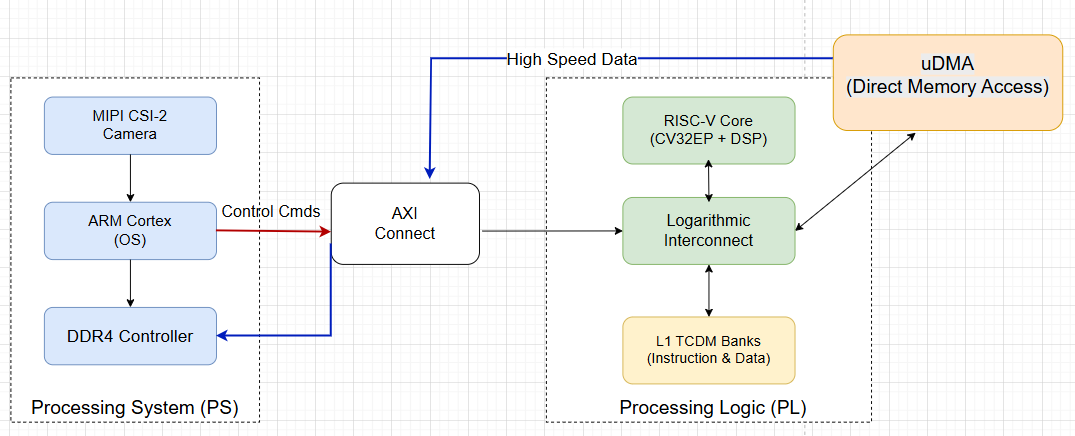
\includegraphics[width=1\textwidth]{chapter04/img/arch.png}
\caption{Kiến trúc hệ thống tổng quan}
\label{fig:proposed_architecture}
\end{figure}

Mô hình tổng thể được chia thành hai miền xử lý chính:
\begin{itemize}
    \item Processing System
    \item Khối Cầu nối
    \item Programmable Logic
\end{itemize}

Như thể hiện tại Hình \ref{fig:proposed_architecture}, hệ thống được phân chia thành ba miền xử lý chính với các vai trò chuyên biệt:

\begin{itemize}
    \item \textbf{Phân hệ Xử lý (Processing System - PS):} 
    Đóng vai trò là khối điều khiển trung tâm (Host), hoạt động trên nền tảng vi xử lý ARM Cortex-A53 lõi tứ. PS chịu trách nhiệm:
    \begin{itemize}
        \item Quản lý tài nguyên hệ thống và khởi chạy quy trình boot.
        \item Giao tiếp với các ngoại vi tiêu chuẩn như Camera (qua giao diện MIPI CSI-2) và Màn hình.
        \item Thực hiện các bước tiền xử lý hình ảnh (Preprocessing) và quản lý bộ nhớ đệm dữ liệu (Data Buffering) trên DDR4.
    \end{itemize}

    \item \textbf{Khối Giao tiếp Liên kết (Interconnect Fabric):} 
    Đóng vai trò là cầu nối dữ liệu tốc độ cao, sử dụng giao thức chuẩn công nghiệp AMBA AXI4. Khối này bao gồm các bộ chuyển mạch thông minh (AXI SmartConnect) để:
    \begin{itemize}
        \item Phân tách luồng điều khiển (Control Plane) băng thông thấp và luồng dữ liệu (Data Plane) băng thông cao.
        \item Đảm bảo đồng bộ hóa giữa hai miền xung nhịp khác nhau của PS và PL.
        \item Cho phép truy cập bộ nhớ chia sẻ (Shared Memory) một cách trong suốt giữa các vi xử lý.
    \end{itemize}

    \item \textbf{Phân hệ Logic Khả trình (Programmable Logic - PL):} 
    Đóng vai trò là bộ tăng tốc tính toán (Accelerator). Tại đây, tài nguyên FPGA được cấu hình để triển khai một Hệ thống trên Chip (SoC) con, bao gồm:
    \begin{itemize}
        \item \textbf{Lõi vi xử lý mềm RISC-V (PULP Subsystem):} Điều phối luồng thực thi thuật toán AI.
        \item \textbf{Bộ tăng tốc phần cứng (CNN Accelerator):} Thực hiện các phép toán tích chập chuyên sâu.
        \item \textbf{Cơ chế truy cập bộ nhớ trực tiếp (uDMA):} Tối ưu hóa việc di chuyển dữ liệu ảnh mà không làm gián đoạn CPU.
    \end{itemize}
\end{itemize}

Sự kết hợp chặt chẽ giữa ba thành phần này cho phép hệ thống hoạt động theo cơ chế đường ống (Pipelining), đảm bảo khả năng xử lý hình ảnh thời gian thực với độ trễ thấp nhất.

%=======================================================================
\newpage
\section{Thiết kế Processing System}

Đây là phần cứng có sẵn (Hard-core) trên chip Zynq UltraScale+ của board Kria KV260.
\begin{itemize}
    \item ARM Cortex-A53: Đóng vai trò là CPU chủ (Host). Nó có thểchạy hệ điều hành (Linux hoặc Bare-metal) 
để quản lý toàn bộ hệ thống. Nhiệm vụ của nó là giao tiếp với Camera (qua cổng MIPI), 
nhận ảnh, tiền xử lý (resize, crop) và lưu trữ ảnh vào bộ nhớ lớn.
    \item DDR4 Controller (Shared Memory): Đây là kho chứa dữ liệu chung. Vì bộ nhớ trong của RISC-V 
rất nhỏ (chỉ vài chục KB), toàn bộ dữ liệu ảnh đầu vào (Image Buffer) phải được lưu ở đây 
(4GB RAM của Kria).
\end{itemize}

PS đóng vai trò "Master" điều phối, gửi lệnh "Bắt đầu" (Start) cho khối PL 
khi đã có dữ liệu ảnh sẵn sàng.

\subsection{Cấu hình chi tiết các phân hệ}

\subsubsection{Khối xử lý ứng dụng (APU Configuration)}
Trung tâm của PS là cụm vi xử lý Quad-core ARM Cortex-A53 hoạt động ở tần số 1.2 GHz. Trong thiết kế này, APU được cấu hình để:
\begin{itemize}
    \item \textbf{Chế độ hoạt động:} Chạy hệ điều hành PetaLinux (dựa trên Yocto Project) để tận dụng các driver có sẵn cho Camera MIPI và ngăn xếp mạng (Network Stack).
    \item \textbf{Quản lý Boot:} Sử dụng giao diện SD Card (SD1) kết nối với các chân MIO để nạp bitstream cho FPGA và khởi động hệ thống.
\end{itemize}

\subsubsection{Cấu hình Giao diện Bộ nhớ (DDR Configuration)}
Bộ điều khiển DDR4 (DDRC) được kích hoạt để quản lý 4GB RAM tích hợp trên Kria SOM. Cấu hình này rất quan trọng vì nó đóng vai trò là "Shared Memory" cho cả hệ thống:
\begin{itemize}
    \item \textbf{Data Width:} 64-bit (hỗ trợ băng thông cao).
    \item \textbf{AXI Port QoS:} Cổng S\_AXI\_HP0 được ưu tiên mức Quality of Service (QoS) cao để đảm bảo uDMA không bị nghẽn khi ghi dữ liệu ảnh, tránh hiện tượng rớt khung hình (frame drop).
\end{itemize}

\subsubsection{Cấu hình Giao diện PS-PL (Interface Configuration)}
Để kết nối với miền Logic khả trình (nơi chứa RISC-V và Accelerator), hai cổng giao tiếp AXI quan trọng được kích hoạt:

\begin{enumerate}
    \item \textbf{M\_AXI\_HPM0\_FPD (Master):}
    \begin{itemize}
        \item \textit{Chức năng:} Cổng Master hiệu năng cao miền công suất thấp (Full Power Domain).
        \item \textit{Nhiệm vụ:} Dùng để CPU ARM gửi tín hiệu điều khiển, cấu hình thanh ghi và nạp firmware vào bộ nhớ lệnh của RISC-V.
        \item \textit{Độ rộng:} 32-bit (phù hợp với bus AXI-Lite).
    \end{itemize}
    
    \item \textbf{S\_AXI\_HP0\_FPD (Slave):}
    \begin{itemize}
        \item \textit{Chức năng:} Cổng Slave hiệu năng cao (High Performance).
        \item \textit{Nhiệm vụ:} Cho phép các Master bên phía FPGA (cụ thể là uDMA) truy cập trực tiếp vào RAM DDR4.
        \item \textit{Độ rộng:} 128-bit (để tối đa hóa tốc độ truyền tải ảnh).
    \end{itemize}
\end{enumerate}

\subsubsection{Cấu hình Xung nhịp (Clock Configuration)}
Khối PS cung cấp nguồn xung nhịp tham chiếu cho toàn bộ logic bên phía PL 
thông qua chân \texttt{pl\_clk0}. Tần số được thiết lập là \textbf{100 MHz}, 
đảm bảo sự cân bằng giữa tốc độ xử lý của nhân RISC-V và mức tiêu thụ năng lượng.

%=========================================================
\newpage
\section{Thiết kế Hệ thống Giao tiếp và Bộ nhớ (Interconnect \& Memory Hierarchy)}
\label{sec:interconnect_design}

Trong kiến trúc SoC dị thể, hiệu năng của hệ thống không chỉ phụ thuộc vào tốc độ xử lý của từng nhân (Core) mà còn phụ thuộc vào băng thông và độ trễ của hệ thống kết nối. Mục này trình bày thiết kế chi tiết mạng lưới giao tiếp giữa PS và PL, cùng với quy hoạch không gian bộ nhớ chung.

\begin{figure}[h]
    \centering
    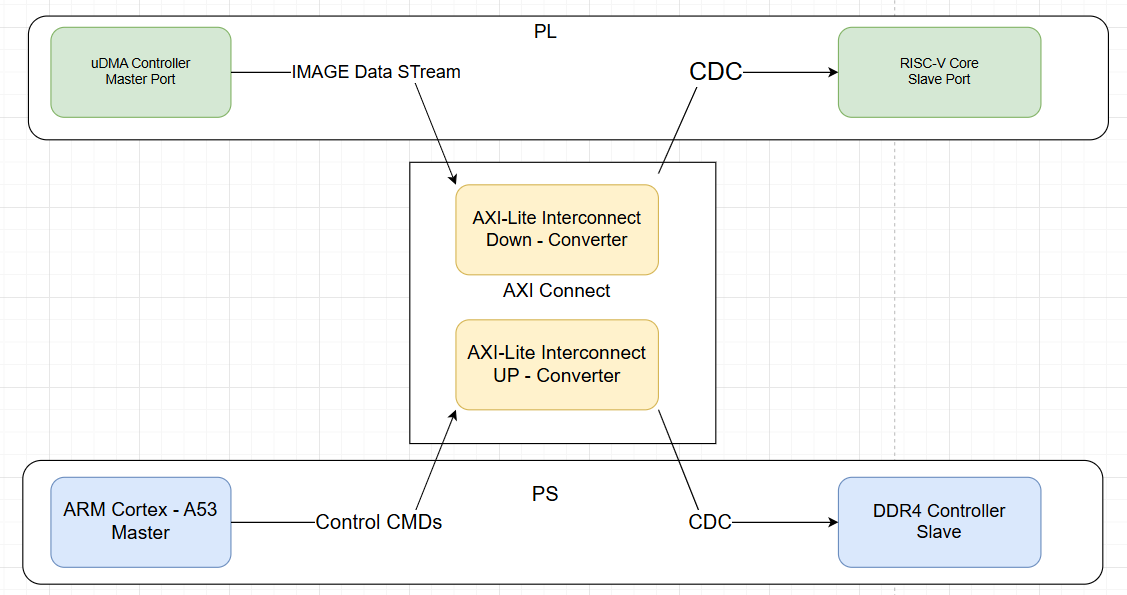
\includegraphics[width=1\textwidth]{chapter04/img/axi_arch.png}  
    \caption{Sơ đồ khối hệ thống giao tiếp AXI giữa PS và PL.}
    \label{fig:axi_interconnect}
\end{figure}


\subsection{Cơ chế AXI SmartConnect (PS-PL Bridge)}
Để kết nối miền xử lý ứng dụng (PS) hoạt động ở tần số cao và miền logic khả trình (PL) hoạt động ở tần số thấp, hệ thống sử dụng khối IP **AXI SmartConnect**. Đây không chỉ là dây dẫn đơn thuần mà là một ma trận chuyển mạch thông minh (Switch Fabric) đảm nhiệm ba chức năng:
\begin{itemize}
    \item \textbf{Clock Domain Crossing (CDC):} Đồng bộ hóa tín hiệu giữa miền xung nhịp PS (1.2 GHz) và miền PL (100 MHz) bằng các bộ đệm FIFO bất đồng bộ, đảm bảo không xảy ra lỗi Metastability.
    \item \textbf{Width Conversion:} Chuyển đổi độ rộng dữ liệu tự động giữa bus hệ thống 128-bit (phía DDR) và bus ngoại vi 32-bit (phía RISC-V).
    \item \textbf{Arbitration:} Phân giải tranh chấp khi nhiều Master cùng truy cập bộ nhớ.
\end{itemize}

Hệ thống được thiết kế với hai kênh giao tiếp vật lý tách biệt:

\subsubsection{Kênh Điều khiển (Control Path - AXI4-Lite)}
Đây là tuyến giao tiếp từ \textbf{Master (ARM Cortex-A53)} đến \textbf{Slave (PULP Subsystem)}.
\begin{itemize}
    \item \textbf{Giao thức:} AXI4-Lite 32-bit. Đây là phiên bản rút gọn của AXI4, không hỗ trợ truyền tải dạng Burst.
    \item \textbf{Mục đích:} Tối ưu hóa cho các giao dịch đơn lẻ, độ trễ thấp.
    \item \textbf{Chức năng:} Dùng để CPU ARM thực hiện các tác vụ quản trị như:
    \begin{itemize}
        \item Cấu hình thanh ghi điều khiển của bộ tăng tốc CNN (Trọng số, Bias, Kích thước ảnh).
        \item Gửi tín hiệu kích hoạt (Trigger) quá trình suy luận.
        \item Reset mềm (Soft-reset) khối PL trong trường hợp treo hệ thống.
    \end{itemize}
\end{itemize}

\subsubsection{Kênh Dữ liệu (Data Path - AXI4-Full)}
Đây là tuyến giao tiếp từ \textbf{Master (uDMA Controller)} đến \textbf{Slave (DDR4 Controller)}.
\begin{itemize}
    \item \textbf{Giao thức:} AXI4-Full 128-bit.
    \item \textbf{Mục đích:} Tối ưu hóa băng thông (Throughput).
    \item \textbf{Chức năng:} Hỗ trợ cơ chế \textit{Burst Transaction}, cho phép uDMA đọc/ghi liên tiếp tới 256 gói dữ liệu chỉ với một địa chỉ bắt đầu. Điều này cực kỳ quan trọng để đảm bảo cung cấp đủ dữ liệu pixel cho mạng MobileNet hoạt động thời gian thực (Real-time).
\end{itemize}

\subsection{Quy hoạch không gian bộ nhớ (System Memory Map)}
\label{sec:memory_map}
Hệ thống quy hoạch không gian bộ nhớ thống nhất giữa hai góc nhìn của lõi RISC-V (32-bit flat) và lõi ARM (PS), với nguyên tắc \textbf{cùng địa chỉ logic} cho cùng một thiết bị slave để đơn giản hóa việc trao đổi con trỏ giữa hai master. Bảng~\ref{tab:memory_map} tổng hợp bản đồ bộ nhớ chi tiết.

\begin{table}[h]
\centering
\caption{Bản đồ bộ nhớ hệ thống (System Memory Map)}
\label{tab:memory_map}
\begin{tabular}{|l|l|l|p{5.5cm}|}
\hline
\textbf{Địa chỉ} & \textbf{Kích thước} & \textbf{Slave} & \textbf{Chức năng} \\ \hline
\multicolumn{4}{|l|}{\textit{Góc nhìn RISC-V (qua \texttt{m\_axi\_instr} + \texttt{m\_axi\_data})}} \\ \hline
\texttt{0x0000\_0000} & 64 KB & I-BRAM Port A & Instruction fetch (\texttt{.text}, \texttt{.rodata}, vector reset). \\ \hline
\texttt{0xB000\_0000} & 64 KB & \texttt{axi\_dma\_0} S\_AXI\_LITE & Thanh ghi điều khiển DMA (MM2S, S2MM, CTRL/STATUS). \\ \hline
\texttt{0xB001\_0000} & 64 KB & \texttt{conv\_cnn\_0} S00\_AXI & Thanh ghi điều khiển bộ tăng tốc CNN (GEOMETRY, CTRL, STATUS, CHANNELS, M\_Q31, SHIFT\_ZP). \\ \hline
\texttt{0xB004\_0000} & 256 KB & D-BRAM Port A & \texttt{.data}, \texttt{.bss}, stack và các thanh ghi handshake chia sẻ với ARM. \\ \hline
\multicolumn{4}{|l|}{\textit{Góc nhìn ARM PS (qua \texttt{M\_AXI\_HPM0/HPM1\_FPD})}} \\ \hline
\texttt{0xA000\_0000} & 64 KB & I-BRAM Port B & ARM nạp/reload \texttt{firmware.bin} vào BRAM lệnh của RISC-V. \\ \hline
\texttt{0xB001\_0000} & 64 KB & \texttt{conv\_cnn\_0} S00\_AXI & ARM cấu hình trực tiếp bộ tăng tốc nếu cần. \\ \hline
\texttt{0xB004\_0000} & 256 KB & D-BRAM Port B & Vùng shared memory ARM $\leftrightarrow$ RISC-V (handshake regs, layer pointers, kết quả). \\ \hline
\multicolumn{4}{|l|}{\textit{Góc nhìn DMA (qua \texttt{S\_AXI\_HPC0\_FPD}, cache-coherent)}} \\ \hline
\texttt{0x0000\_0000} & 2 GB & DDR\_LOW & IFM/Weights/OFM buffers cấp phát bởi ARM qua \texttt{pynq.allocate} (CMA). \\ \hline
\end{tabular}
\end{table}

Đặc điểm thiết kế quan trọng:
\begin{itemize}
    \item \textbf{I-BRAM ánh xạ kép} (\texttt{0x0000\_0000} từ RISC-V, \texttt{0xA000\_0000} từ ARM): cho phép ARM nạp lại firmware mà không cần halt RISC-V.
    \item \textbf{D-BRAM ánh xạ đồng địa chỉ} (\texttt{0xB004\_0000} từ cả hai phía): tiện cho debug lock-step và trao đổi pointer trực tiếp.
    \item \textbf{Bộ nhớ DDR riêng cho DMA}: vùng DDR\_LOW chỉ được DMA truy cập (đã \textit{Exclude} BRAM khỏi DMA route trong Vivado Address Editor để tránh xung đột); ARM chỉ định địa chỉ vật lý qua \texttt{pynq.allocate} và truyền pointer xuống RISC-V qua D-BRAM.
\end{itemize}

\subsubsection{Bố cục thanh ghi handshake trong D-BRAM Port B}
\label{sec:handshake_regs}
Thay vì sử dụng một thanh ghi mailbox đơn lẻ, đề tài thiết kế một bố cục thanh ghi nhiều trường tại đầu vùng D-BRAM Port B (offset từ \texttt{0xB004\_0000}) để trao đổi đầy đủ thông tin điều khiển và kết quả. Bảng~\ref{tab:shared_regs} mô tả layout các thanh ghi:

\begin{table}[h]
\centering
\caption{Bố cục thanh ghi chia sẻ trong D-BRAM Port B}
\label{tab:shared_regs}
\begin{tabular}{|l|l|p{2.2cm}|p{6cm}|}
\hline
\textbf{Offset} & \textbf{Tên} & \textbf{Hướng} & \textbf{Mô tả} \\ \hline
\texttt{+0x00} & \texttt{CMD\_FROM\_ARM} & ARM $\to$ RISC-V & \texttt{0x01} = START, \texttt{0x00} = idle. \\ \hline
\texttt{+0x04} & \texttt{STATUS\_TO\_ARM} & RISC-V $\to$ ARM & \texttt{0x00} IDLE / \texttt{0x01} BUSY / \texttt{0x02} DONE. \\ \hline
\texttt{+0x08} & \texttt{DATASET\_ID} & ARM $\to$ RISC-V & 0 = INRIA, 1 = Cats vs Dogs. \\ \hline
\texttt{+0x0C} & \texttt{RESULT\_CLASS} & RISC-V $\to$ ARM & Kết quả argmax (tùy chọn; mặc định ARM tự argmax). \\ \hline
\texttt{+0x10} & \texttt{RESULT\_CONF} & RISC-V $\to$ ARM & Confidence Q1.7 (tùy chọn). \\ \hline
\texttt{+0x18} & \texttt{IFM\_PHYS\_ADDR} & ARM $\to$ RISC-V & Địa chỉ vật lý DDR của buffer A (IFM, ping-pong scratch). \\ \hline
\texttt{+0x1C} & \texttt{OFM\_PHYS\_ADDR} & ARM $\to$ RISC-V & Địa chỉ vật lý DDR của buffer B (ping-pong scratch / OFM cuối). \\ \hline
\texttt{+0x20} & \texttt{WEIGHT\_BASE} & ARM $\to$ RISC-V & Địa chỉ vật lý DDR của blob weights; RISC-V cộng \texttt{LAYERS[i].weight\_offset} để ra phys addr per-layer. \\ \hline
\end{tabular}
\end{table}

\subsubsection{Cơ chế Đồng bộ hóa}
Quy trình bắt tay giữa ARM và RISC-V cho mỗi lần inference được mô tả như sau:
\begin{enumerate}
    \item \textbf{ARM (chuẩn bị):} Cấp phát các CMA buffer cho weights, IFM ping-pong A, IFM ping-pong B; ghi pixel ảnh đã lượng tử hóa vào buffer A; ghi 3 thanh ghi địa chỉ \texttt{IFM\_PHYS\_ADDR}, \texttt{OFM\_PHYS\_ADDR}, \texttt{WEIGHT\_BASE}.
    \item \textbf{ARM (kích hoạt):} Ghi \texttt{0x01} vào \texttt{CMD\_FROM\_ARM}.
    \item \textbf{RISC-V (xử lý):} Polling \texttt{CMD\_FROM\_ARM}; khi thấy \texttt{0x01} thì duyệt mảng \texttt{LAYERS[]}, với mỗi layer cấu hình DMA (MM2S đọc IFM/weights, S2MM ghi OFM), cấu hình \texttt{conv\_cnn\_0/S00\_AXI}, kích hoạt và đợi xong.
    \item \textbf{RISC-V (báo hoàn thành):} Sau layer cuối, ghi \texttt{STATUS\_TO\_ARM = 0x02} (DONE).
    \item \textbf{ARM (đọc kết quả):} Polling \texttt{STATUS\_TO\_ARM}; khi DONE, gọi \texttt{.invalidate()} trên buffer cuối, đọc OFM, thực hiện GAP + softmax + argmax bằng phần mềm để có nhãn cuối cùng. Reset \texttt{CMD\_FROM\_ARM} về \texttt{0x00} để chuẩn bị cho frame tiếp theo.
\end{enumerate}


%=============================================
%
%=============================================
\newpage
\section{Thiết kế Programmable Logic}
\label{sec:pl_design}

Logic Khả trình (PL) được thiết kế như một Hệ thống trên Chip (SoC) thu nhỏ hoạt động độc lập, dựa trên kiến trúc mở PULPissimo. Mục tiêu của phân hệ này là tạo ra một môi trường tính toán hiệu năng cao, độ trễ thấp để thực thi các tác vụ điều khiển và tăng tốc AI, giảm tải cho vi xử lý chính ARM.

\subsection{Kiến trúc tổng thể Phân hệ PULP (PULP Subsystem)}
Hình \ref{fig:pulp_arch} trình bày sơ đồ kiến trúc chi tiết của khối PL. Thiết kế bao gồm ba thành phần cốt lõi: Lõi xử lý RISC-V, Hệ thống bộ nhớ TCDM phân tán, và Bộ điều khiển uDMA, được kết nối với nhau thông qua một mạng lưới giao tiếp băng thông rộng (Logarithmic Interconnect).

\begin{figure}[h]
    \centering
    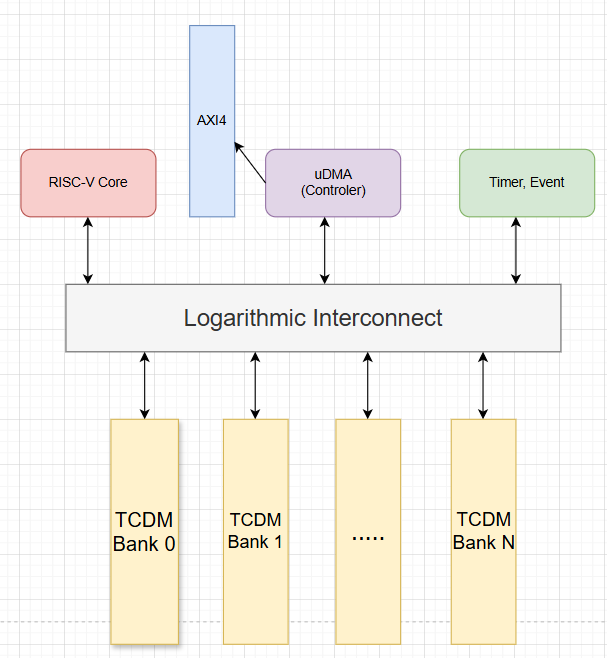
\includegraphics[width=0.8\textwidth]{chapter04/img/pulp_arch.png}  
    \caption{Sơ đồ kiến trúc nội bộ của Phân hệ PULP trên FPGA.}
    \label{fig:pulp_arch}
\end{figure}

\subsection{Cấu hình Nhân Vi xử lý (RISC-V Core Configuration)}
Trung tâm điều khiển của PL là lõi IP RISC-V (dựa trên nhân CV32E40P). Lõi này được tham số hóa trước khi tổng hợp (Synthesis) để đạt sự cân bằng tối ưu giữa tài nguyên FPGA (LUTs) và hiệu năng tính toán:

\begin{table}[h]
\centering
\caption{Thông số cấu hình RISC-V Soft-core}
\label{tab:riscv_config}
\begin{tabular}{|l|l|p{6cm}|}
\hline
\textbf{Tham số} & \textbf{Giá trị} & \textbf{Ý nghĩa thiết kế} \\ \hline
Architecture & RV32IMCXpulp & Hỗ trợ tập lệnh nhân (M), nén (C) và mở rộng DSP/SIMD (Xpulp) cho AI. \\ \hline
Pipeline Stages & 4 & Đủ sâu để đạt tần số 100MHz, đủ ngắn để giảm độ trễ rẽ nhánh. \\ \hline
FPU & Disabled & Không sử dụng bộ xử lý dấu phẩy động để tiết kiệm diện tích (MobileNet đã được lượng tử hóa sang INT8). \\ \hline
Instruction Cache & 4 KB & Kiểu Direct Mapped, giúp CPU nạp lệnh nhanh mà không cần truy cập RAM ngoài liên tục. \\ \hline
Boot Address & \texttt{0x1A00\_0000} & Vị trí vector ngắt khởi động, trỏ tới vùng nhớ ROM khởi tạo. \\ \hline
\end{tabular}
\end{table}

\subsection{Hệ thống Bộ nhớ TCDM và Interconnect}
Điểm yếu chí tử của các hệ thống đa vi xử lý là hiện tượng tranh chấp bộ nhớ (Memory Contention). Thiết kế này giải quyết triệt để vấn đề trên bằng kiến trúc TCDM (Tightly Coupled Data Memory).

\subsubsection{Tổ chức Bộ nhớ Đan xen (Interleaved Memory Banking)}
Thay vì sử dụng một khối Block RAM khổng lồ đơn nhất (64KB), bộ nhớ TCDM được chia nhỏ thành \textbf{16 ngân hàng (Banks)}, mỗi ngân hàng có dung lượng 4KB.
\begin{itemize}
    \item \textbf{Nguyên lý:} Các địa chỉ liên tiếp nhau ($Addr, Addr+4, Addr+8...$) được lưu trữ lần lượt trên các Bank khác nhau ($Bank_0, Bank_1, Bank_2...$).
    \item \textbf{Lợi ích:} Cho phép truy cập song song. Ví dụ: RISC-V Core có thể đọc dữ liệu tại địa chỉ $A$ (nằm ở Bank 0) cùng lúc uDMA ghi dữ liệu vào địa chỉ $B$ (nằm ở Bank 1) mà không hề xảy ra xung đột.
\end{itemize}

\subsubsection{Logarithmic Interconnect}
Kết nối giữa các Master (Core, uDMA) và các Slave (Memory Banks) không phải là một Bus tuyến tính mà là một \textbf{Ma trận chuyển mạch (Switch Matrix)}.
\begin{itemize}
    \item Mạng lưới này có độ trễ cực thấp (chỉ 1 chu kỳ xung nhịp).
    \item Đảm bảo băng thông cực đại: Tổng băng thông nội bộ có thể đạt tới $N \times 32$-bit/cycle (với N là số lượng Bank).
\end{itemize}

\subsection{Cơ chế Truy cập Bộ nhớ Trực tiếp (uDMA)}
Để giải phóng CPU khỏi tác vụ sao chép dữ liệu nhàm chán, một bộ điều khiển uDMA (Micro-DMA) chuyên dụng được tích hợp:
\begin{itemize}
    \item \textbf{Chức năng:} uDMA đóng vai trò cầu nối giữa các ngoại vi tốc độ cao (như AXI4 port nối tới DDR4, SPI, Camera) và bộ nhớ TCDM.
    \item \textbf{Double Buffering:} uDMA hỗ trợ cấu hình hai vùng đệm (Buffer A và Buffer B). Khi đang xử lý dữ liệu ở Buffer A, uDMA sẽ tự động tải dữ liệu mới vào Buffer B trong nền (Background).
    \item \textbf{Kết nối với Accelerator:} uDMA cung cấp một luồng dữ liệu liên tục (Stream) cho khối tăng tốc CNN thông qua giao diện AXI-Stream, đảm bảo bộ tăng tốc luôn có dữ liệu để tính toán (tránh hiện tượng Starvation).
\end{itemize}

%=============================================================
\newpage
\section{Thiết kế Khối Tăng tốc phần cứng (CNN Accelerator)}
Nằm trong PL, khối tăng tốc CNN được thiết kế để thực hiện các phép toán tích chập
một cách song song và hiệu quả. Thiết kế này bao gồm các thành phần chính \cite{fpga2}
\label{sec:cnn_accelerator}

Đây là thành phần cốt lõi quyết định hiệu năng của toàn bộ hệ thống Edge-AI. 
Để đáp ứng yêu cầu tính toán thời gian thực của mạng MobileNetV1, nhóm thực hiện thiết kế một bộ tăng tốc phần cứng chuyên dụng (Domain-Specific Architecture - DSA) được tích hợp trong miền Logic khả trình (PL).
Khối tăng tốc này được thiết kế để giảm tải (offload) các phép toán tích 
chập nặng nề nhất khỏi vi xử lý RISC-V, hoạt động theo cơ chế dòng dữ liệu 
(Dataflow) để tối đa hóa thông lượng.

\subsection{Kiến trúc tổng quát khối Accelerator}
Sơ đồ khối chức năng của bộ tăng tốc được mô tả trong Hình \ref{fig:accel_arch}. Khối này giao tiếp với hệ thống thông qua hai giao diện chính:

\begin{figure}[h]
\centering
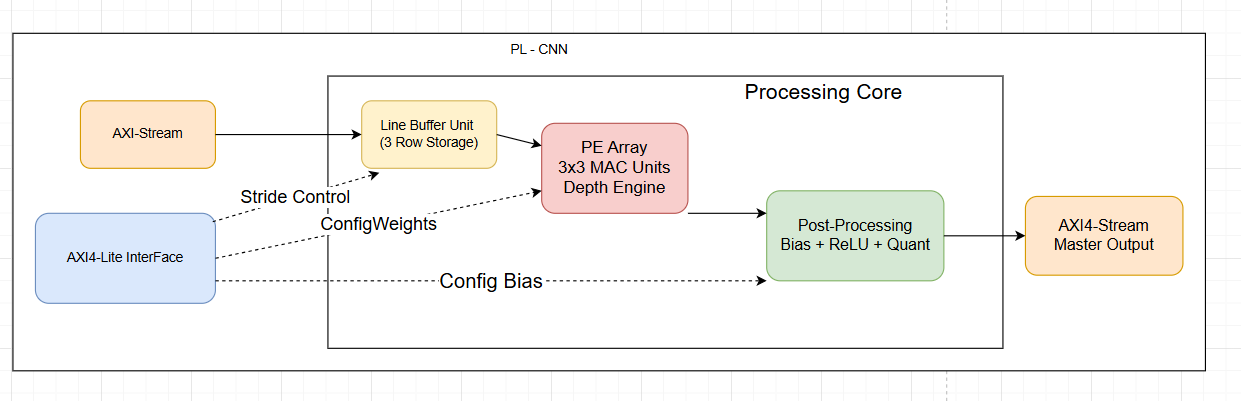
\includegraphics[width=1\textwidth]{chapter04/img/cnn_acce.png}
\caption{Sơ đồ khối chức năng chi tiết của bộ tăng tốc CNN (Accelerator Core Architecture).}
\label{fig:accel_arch}
\end{figure}

\begin{itemize}
    \item \textbf{AXI4-Stream Slave:} Nhận dòng pixel ảnh đầu vào từ uDMA hoặc trực tiếp từ bộ nhớ đệm.
    \item \textbf{AXI4-Stream Master:} Đẩy dòng kết quả (Feature Maps) sau khi tính toán trở lại bộ nhớ.
\end{itemize}

\subsection{Các thành phần chức năng chi tiết}

\subsubsection{Bộ đệm dòng (Line Buffer)}
Để thực hiện tích chập $3 \times 3$, tại mỗi thời điểm cần truy cập đồng thời 3 hàng pixel liên tiếp. Nếu đọc trực tiếp từ DDR cho mỗi lần trượt cửa sổ thì băng thông sẽ trở thành điểm nghẽn. Thiết kế sử dụng \textit{line buffer} hai-bank dựa trên BRAM nội bộ với cơ chế \textit{read-before-write parity-toggled}: khi một pixel mới được nạp vào bank này thì 2 hàng cũ vẫn được giữ ở bank kia. Cùng với khối \texttt{window\_3x3} đứng sau (mảng thanh ghi $3 \times 3 \times \texttt{cin}$), thiết kế tái sử dụng dữ liệu cục bộ và giảm số lần truy xuất bộ nhớ ngoài xuống còn 1 lần/pixel.

\subsubsection{Mảng tính toán PE và adder tree}
Trung tâm tính toán của bộ tăng tốc gồm 9 PE (Processing Element) MAC (Multiply-Accumulate) hoạt động song song, tương ứng với 9 vị trí của kernel $3 \times 3$:
\begin{itemize}
    \item Mỗi PE thực hiện phép nhân INT8$\times$INT8 và cộng dồn vào thanh ghi tích lũy 32-bit. Cấu trúc pipelined với MREG + PREG cho phép Vivado ánh xạ trực tiếp vào khối DSP48E2.
    \item Đầu ra của 9 PE được tổng hợp qua \textit{adder tree} 4-tầng để cho ra một giá trị tích chập 32-bit cho mỗi nhóm 9 pixel + 9 trọng số.
    \item Đối với layer có nhiều kênh đầu vào ($\texttt{cin} > 1$), bộ điều khiển sử dụng cơ chế \textit{channel-interleaved per pixel}: tích lũy qua \texttt{cin} kênh trước khi xuất ra giá trị OFM cho mỗi tổ hợp $(y, x, \texttt{cnt\_cout})$.
\end{itemize}

\subsubsection{Khối lượng tử hóa (Requantize)}
Sau khi tổng chập, kết quả 32-bit cần được \textit{re-quantize} về INT8 để khớp định dạng đầu vào của layer kế tiếp. Khối \texttt{requantize.sv} thực hiện đường ống 3-tầng theo công thức TFLite \cite{jacob2018quantization}:
\begin{equation}
    y_q = \mathrm{sat}_{\mathrm{INT8}}\!\left( \left\lfloor \frac{(\sum x \cdot w + b) \cdot M_{q31} + 2^{30+n}}{2^{31+n}} \right\rfloor + z_{\mathrm{out}} \right)
\end{equation}
trong đó $M_{q31}$ là hệ số nhân Q31 (\texttt{int32}), $n$ là số bit dịch phải ($n \in [0, 31]$), $z_{\mathrm{out}}$ là zero-point đầu ra. Cờ \texttt{has\_relu} điều khiển việc kẹp giá trị âm về 0 (fused ReLU). Hệ số $M_{q31}$ và $n$ được tính sẵn trong pipeline huấn luyện và truyền xuống qua thanh ghi S00\_AXI cho từng layer.

\subsection{Đặc tính thiết kế và tối ưu cho vgg-tiny}
\label{sec:accel_optimize}
Thay vì cố gắng tổng quát hóa hỗ trợ tất cả các loại mạng CNN, đề tài chọn \textbf{thu hẹp tập op} mà bộ tăng tốc hỗ trợ trong phiên bản v2.0 alpha để đảm bảo tiến độ và tính đúng đắn:
\begin{itemize}
    \item Hỗ trợ Conv 3$\times$3 với padding VALID, stride 1, hàm kích hoạt ReLU (fused).
    \item Hỗ trợ tới \texttt{MAX\_CIN} = 64 và \texttt{MAX\_COUT} = 64 kênh trên mỗi layer (tham số hóa trong \texttt{conv\_pkg.sv}).
    \item Hỗ trợ runtime-configurable cho geometry ($W \times H$), số kênh, hệ số lượng tử hóa qua thanh ghi điều khiển AXI4-Lite.
\end{itemize}

Lựa chọn này dẫn đến mô hình triển khai chính là \texttt{vgg-tiny} -- một mạng \textit{fully-convolutional} đơn giản chỉ dùng các op nói trên (mục~\ref{sec:vgg_tiny}). Các kiến trúc phức tạp hơn như Pointwise 1$\times$1, Depthwise, Stride 2, Padding SAME, hay Residual Add được dành cho các pha mở rộng tương lai trong roadmap (mục~\ref{sec:tier_roadmap}).

%=============================================================
%
%=============================================================
\newpage
\section{Mô hình AI mục tiêu: vgg-tiny}
\label{sec:ai_algorithm}

Việc lựa chọn mô hình AI chạy trên hệ thống phải cân bằng giữa hai yếu tố: (i) tập op mà bộ tăng tốc Conv-CNN v2.0 hỗ trợ (xem mục~\ref{sec:accel_optimize}) và (ii) độ chính xác đủ tốt cho bài toán phân loại nhị phân. Đề tài đề xuất một kiến trúc tinh gọn riêng tên \texttt{vgg-tiny} -- lấy cảm hứng từ phong cách VGG (chỉ dùng Conv $3 \times 3$ stacking) nhưng được rút gọn để chạy được hoàn toàn trên phần cứng đã thiết kế.

\subsection{Đặc tả kiến trúc vgg-tiny}
\label{sec:vgg_tiny}
\texttt{vgg-tiny} là một mạng \textit{fully-convolutional} 5 layer, đầu vào ảnh RGB $128 \times 128$, output là tensor 2 kênh được ARM thực hiện Global Average Pooling + softmax + argmax thành nhãn cuối cùng. Bảng~\ref{tab:vgg_tiny_layers} mô tả cấu trúc chi tiết.

\begin{table}[h]
\centering
\caption{Cấu trúc chi tiết các lớp mạng vgg-tiny (đầu vào $128 \times 128 \times 3$, lượng tử hóa INT8)}
\label{tab:vgg_tiny_layers}
\begin{tabular}{|c|l|c|c|c|c|}
\hline
\textbf{Layer} & \textbf{Loại op} & \textbf{IFM} & \textbf{OFM} & \textbf{Kernel} & \textbf{Activation} \\ \hline
L0 & Conv2D + ReLU & $128 \times 128 \times 3$ & $126 \times 126 \times 8$ & $3 \times 3$ & ReLU \\ \hline
L1 & Conv2D + ReLU & $126 \times 126 \times 8$ & $124 \times 124 \times 16$ & $3 \times 3$ & ReLU \\ \hline
L2 & Conv2D + ReLU & $124 \times 124 \times 16$ & $122 \times 122 \times 32$ & $3 \times 3$ & ReLU \\ \hline
L3 & Conv2D + ReLU & $122 \times 122 \times 32$ & $120 \times 120 \times 64$ & $3 \times 3$ & ReLU \\ \hline
L4 & Conv2D (logits) & $120 \times 120 \times 64$ & $118 \times 118 \times N$ & $3 \times 3$ & None \\ \hline
\multicolumn{6}{|l|}{\textit{Hậu xử lý trên ARM:} GAP $\to$ softmax $\to$ argmax $\to$ nhãn ($N = $ số lớp = 2)} \\ \hline
\end{tabular}
\end{table}

Các đặc điểm chính:
\begin{itemize}
    \item \textbf{Tất cả op đều thuộc tập hỗ trợ của bộ tăng tốc:} Conv $3 \times 3$, padding VALID, stride 1, ReLU fused. Layer cuối cùng (\texttt{L4}) tắt activation để xuất logits cho softmax trên ARM.
    \item \textbf{Không có Dense head:} Layer cuối là Conv $3 \times 3$ với $\texttt{cout} = N$ (số lớp), thay vì Conv $\to$ Flatten $\to$ Dense kiểu VGG truyền thống. Cách này loại bỏ nhu cầu phần cứng hỗ trợ Fully Connected layer.
    \item \textbf{Không có MaxPool} trong v2.0 alpha: kích thước feature map giảm dần qua valid-padding ($-2$ pixel mỗi chiều). Kết quả là feature map cuối tương đối lớn ($118 \times 118$) và latency cao hơn so với phiên bản có pool. Việc bổ sung MaxPool 2$\times$2 hoặc Conv stride-2 được dành cho V2.1.
    \item \textbf{Số tham số nhỏ:} Tổng cộng $\approx 25,700$ tham số INT8 (xem chi tiết tại bảng~\ref{tab:vgg_tiny_perlayer} trong chương~\ref{chp:06}), dung lượng weights blob khoảng 25 KB -- nằm gọn trong bộ nhớ DDR và dễ quản lý.
\end{itemize}

\subsection{So sánh vgg-tiny với các mô hình thông dụng}
Để minh chứng cho lựa chọn thiết kế, bảng~\ref{tab:model_comparison} so sánh \texttt{vgg-tiny} với các kiến trúc CNN phổ biến trên cùng tiêu chí:

\begin{table}[h]
\centering
\caption{So sánh vgg-tiny với các mạng CNN phổ biến}
\label{tab:model_comparison}
\resizebox{\textwidth}{!}{%
\begin{tabular}{|l|c|c|r|r|r|c|}
\hline
\textbf{Mô hình} & \textbf{Input} & \textbf{Số layer} & \textbf{Params} & \textbf{INT8 size} & \textbf{MACs} & \textbf{FPGA-deployable} \\ \hline
\texttt{vgg-tiny} & $128 \times 128$ & 5 & 25.7K & 25.1 KB & 371 M & \cmark \\ \hline
VGG11 / VGG16 & $224 \times 224$ & 13 & 14.7M & 14.4 MB & 15{,}347 M & \xmark{} (FC head + pool stride-2) \\ \hline
ResNet-18 (V2) & $224 \times 224$ & 53 & 23.6M & 23.0 MB & 3{,}480 M & \xmark{} (1$\times$1 + BN + residual) \\ \hline
EfficientNet-B0 & $224 \times 224$ & 81 & 4.05M & 3.96 MB & 385 M & \xmark{} (depthwise + SE + swish) \\ \hline
MobileNetV1/V2 & $224 \times 224$ & 28 & 2.3--4.2M & 2.2--4.0 MB & 300--569 M & \xmark{} (depthwise) \\ \hline
\end{tabular}%
}
\end{table}

So với các mô hình thương mại, \texttt{vgg-tiny} nhỏ gọn hơn từ 100$\times$ đến 900$\times$ về số tham số, đồng thời tránh được hoàn toàn các op khó (depthwise, BN, residual, SE). Đánh đổi là không gian biểu diễn (representation capacity) hạn chế, phù hợp với bài toán phân loại nhị phân nhưng chưa đủ cho bài toán phân loại nhiều lớp phức tạp như ImageNet 1000 classes.

\subsection{Lộ trình mở rộng (Tier Roadmap)}
\label{sec:tier_roadmap}
Đề tài định hướng triển khai mở rộng theo ba tier, với \texttt{vgg-tiny} là Tier 1 (đã xong), Tier 2--3 là các pha mở rộng:

\begin{itemize}
    \item \textbf{Tier 1 -- vgg-tiny (đã triển khai):} Chỉ Conv $3 \times 3$ stride-1 valid + ReLU. Bộ tăng tốc v2.0 alpha.
    \item \textbf{Tier 2 -- VGG11 / ResNet-18 (mở rộng):} Bổ sung MaxPool 2$\times$2 (hoặc stride-2 conv), padding SAME, 1$\times$1 conv, residual addition. Yêu cầu mở rộng \texttt{conv\_core.sv} và \texttt{controller\_fsm.sv} nhưng không thay đổi giao thức AXI hay layer table contract.
    \item \textbf{Tier 3 -- ResNet-50 / YOLOv3-Tiny (stretch):} Thêm BN folding offline, leaky-ReLU, upsample $2\times$ cho detection head.
\end{itemize}

Mọi mở rộng đều \textbf{không phá vỡ ABI v2.0}: chỉ cần thêm enum cho \texttt{activation\_t}/\texttt{padding\_t}/\texttt{kernel\_size} trong \texttt{layer\_desc.h} và thêm 1 mode-bit ở conv\_core MUX. Pipeline huấn luyện và phần mềm host không cần thay đổi.

\subsection{Lượng tử hóa (Quantization)}
Vi xử lý RISC-V và Khối tăng tốc phần cứng trên FPGA được thiết kế để xử lý số nguyên (Integer Arithmetic) nhằm tối đa hóa tốc độ và tiết kiệm bộ nhớ. Do đó, mô hình gốc (Float32) cần trải qua quy trình \textit{Post-training Quantization}:

\begin{itemize}
    \item \textbf{Weights (Trọng số):} Chuyển đổi từ \texttt{float32} (4 bytes) sang \texttt{int8} (1 byte).
    \item \textbf{Activations (Giá trị kích hoạt):} Đầu ra của mỗi lớp cũng được ép về \texttt{int8}.
    \item \textbf{Bias (Hệ số chệch):} Lưu trữ dưới dạng \texttt{int32} để tránh tràn số (overflow) khi cộng dồn, sau đó được dịch bit (bit-shift) để quay về \texttt{int8}.
\end{itemize}

Công thức lượng tử hóa tổng quát được áp dụng:
\begin{equation}
    R = S(Q - Z)
\end{equation}
Trong đó $R$ là giá trị thực (Real value), $Q$ là giá trị lượng tử hóa (Quantized value), $S$ là tỷ lệ (Scale) và $Z$ là điểm không (Zero-point).

\subsection{Tổ chức Dữ liệu trong Bộ nhớ}
Để tối ưu hóa cho việc truy cập Burst qua AXI4 Bus (128-bit width), các ma trận trọng số (Weights) không được lưu trữ theo thứ tự tuyến tính thông thường mà được sắp xếp lại (Memory Packing):
\begin{itemize}
    \item \textbf{Kernel Layout:} Các bộ lọc được sắp xếp theo cấu trúc \texttt{OHWI} 
    (Output-Height-Width-Input) để đảm bảo khi uDMA đọc 16 bytes (128-bit) sẽ thu được 
    đủ dữ liệu cho các bộ nhân hoạt động song song.
    \item \textbf{C-Header Generation:} File mô hình \texttt{.tflite} cuối cùng được
     chuyển đổi (dump) thành các mảng hằng số trong ngôn ngữ C (\texttt{weights.h})
      để biên dịch cùng với Firmware của RISC-V.
\end{itemize}

%=============================================================
\section{Luồng thực thi và Giao thức bắt tay}
\label{sec:system_flow}

Trong kiến trúc dị thể, việc đồng bộ hóa giữa vi xử lý ARM (chạy Linux + PYNQ runtime) và lõi RISC-V (chạy bare-metal) là yếu tố quyết định tính đúng đắn của hệ thống. Đề tài sử dụng cơ chế bắt tay dựa trên các thanh ghi trạng thái trong D-BRAM Port B (đã trình bày tại mục~\ref{sec:handshake_regs}). Phần này mô tả luồng thực thi end-to-end cho một lần inference.

\paragraph{Quy trình inference một ảnh}
Quá trình thực thi diễn ra qua 4 pha tuần tự, được minh họa trong sơ đồ tuần tự Hình~\ref{fig:sequence_diagram}:

\begin{enumerate}
    \item \textbf{Pha 1 -- ARM chuẩn bị dữ liệu:}
    \begin{itemize}
        \item ARM đọc ảnh \texttt{.jpg}/\texttt{.png} từ thẻ nhớ SD bằng \texttt{cv2.imread}.
        \item Tiền xử lý: chuyển BGR$\to$RGB, resize về $128 \times 128$, chuẩn hóa $[0,1]$.
        \item Lượng tử hóa INT8 theo công thức $q = \mathrm{round}(x / S_{\mathrm{in}}) + Z_{\mathrm{in}}$ với $S_{\mathrm{in}}, Z_{\mathrm{in}}$ đọc từ \texttt{meta.json}.
        \item Cấp phát ba CMA buffer qua \texttt{pynq.allocate}: \texttt{wbuf} (weights), \texttt{buf\_a} (IFM ping-pong), \texttt{buf\_b} (scratch ping-pong); ghi pixel ảnh đã lượng tử vào \texttt{buf\_a} và gọi \texttt{flush()}.
        \item Ghi 3 thanh ghi địa chỉ vật lý \texttt{IFM\_PHYS\_ADDR}, \texttt{OFM\_PHYS\_ADDR}, \texttt{WEIGHT\_BASE} và \texttt{DATASET\_ID} vào D-BRAM Port B (mục~\ref{sec:handshake_regs}).
    \end{itemize}

    \item \textbf{Pha 2 -- ARM kích hoạt RISC-V:}
    \begin{itemize}
        \item Ghi \texttt{0x01} (START) vào \texttt{CMD\_FROM\_ARM @ 0xB004\_0000}.
        \item ARM chuyển sang chế độ chờ (polling \texttt{STATUS\_TO\_ARM} hoặc đợi IRQ).
    \end{itemize}

    \item \textbf{Pha 3 -- RISC-V điều phối tính toán:}
    \begin{itemize}
        \item RISC-V phát hiện \texttt{CMD\_FROM\_ARM == 0x01}, ghi \texttt{STATUS\_TO\_ARM = 0x01} (BUSY).
        \item Duyệt mảng \texttt{LAYERS[]} (compile-in trong I-BRAM): với mỗi layer $i$:
        \begin{itemize}
            \item Tính địa chỉ vật lý weight = \texttt{WEIGHT\_BASE + LAYERS[i].weight\_offset}; ping-pong: \texttt{in = (i\&1)?buf\_b:buf\_a}, \texttt{out = ngược lại}.
            \item Cấu hình \texttt{conv\_cnn\_0/S00\_AXI}: ghi geometry, channels, $M_{q31}$, shift, zero-point, có ReLU; chuyển sang chế độ load weight.
            \item Lập trình \texttt{axi\_dma\_0}: MM2S đọc weights từ DDR $\to$ \texttt{conv\_cnn\_0/S00\_AXIS}; chờ done.
            \item Chuyển sang chế độ infer; lập trình DMA tiếp: MM2S đọc IFM, S2MM ghi OFM về DDR; chờ done.
        \end{itemize}
        \item Sau layer cuối, ghi \texttt{STATUS\_TO\_ARM = 0x02} (DONE).
    \end{itemize}

    \item \textbf{Pha 4 -- ARM hậu xử lý:}
    \begin{itemize}
        \item ARM phát hiện \texttt{STATUS\_TO\_ARM == 0x02}, gọi \texttt{.invalidate()} trên buffer chứa OFM cuối (xác định bởi \texttt{final\_ofm\_buf\_idx} trong \texttt{meta.json}).
        \item Thực hiện Global Average Pool trên trục $(H, W)$ của tensor INT8 OFM, sau đó dequantize về float, áp dụng softmax, lấy argmax để có nhãn cuối cùng.
        \item Hiển thị kết quả lên notebook (matplotlib overlay), in ra console hoặc lưu file log.
        \item Ghi \texttt{CMD\_FROM\_ARM = 0x00} (IDLE) để sẵn sàng cho ảnh tiếp theo.
    \end{itemize}
\end{enumerate}

\begin{figure}[!h]
    \centering
    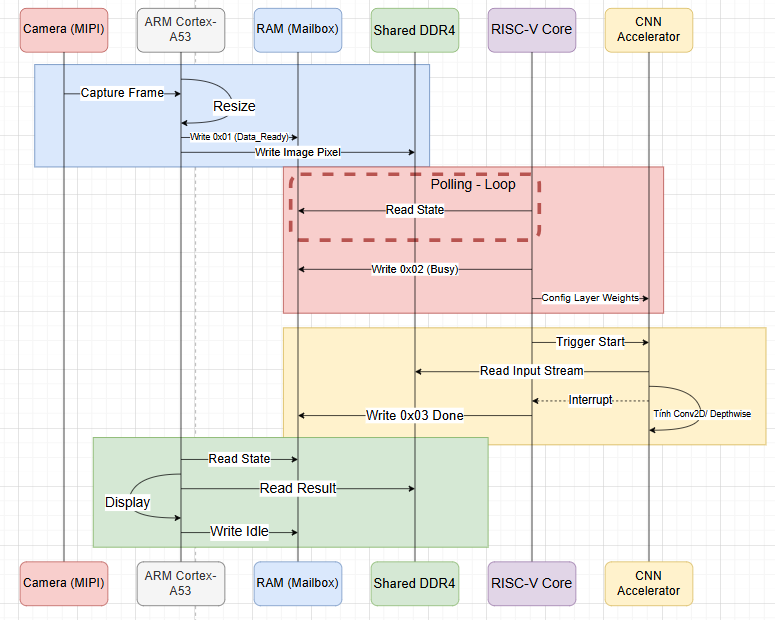
\includegraphics[width=1\textwidth]{chapter04/img/flow.png}
    \caption{Sơ đồ quy trình}
    \label{fig:sequence_diagram}
\end{figure}
\chapter{Hiện thực và kiểm thử hệ thống}
\label{chp:05}


Chương này trình bày chi tiết quá trình hiện thực hóa kiến trúc phần cứng đã đề xuất ở các chương trước thành hệ thống vật lý trên nền tảng FPGA. Nội dung bao gồm việc tinh chỉnh lõi vi xử lý RISC-V, thiết kế cầu nối giao tiếp, tổng hợp bộ gia tốc phần cứng cho mạng nơ-ron, lập trình phần mềm nhúng điều khiển và quy trình huấn luyện, lượng tử hóa mô hình trí tuệ nhân tạo.

\section{Tổng quan hướng hiện thực}
Hệ thống gia tốc AI tại biên (Edge-AI) trong đồ án này được thiết kế theo phương pháp đồng thiết kế phần cứng/phần mềm (Hardware-Software Co-design) mang tính dị cấu trúc (Heterogeneous). Để đảm bảo tính linh hoạt (linh hoạt thay đổi mô hình AI mà không cần tổng hợp lại phần cứng) và hiệu năng cao, hệ thống được hiện thực hóa theo mô hình phân tầng kiến trúc (Layered Architecture) gồm 4 tầng (Layer) phối hợp chặt chẽ với nhau:

\begin{itemize}
    \item \textbf{Layer 1 -- Data Plane (RTL):} Bộ tăng tốc \texttt{conv\_cnn} hiện thực bằng SystemVerilog, thực thi tích chập $3 \times 3$ INT8 + requantize TFLite.
    \item \textbf{Layer 2 -- Orchestrator (Bare-metal C):} Firmware chạy trên lõi RISC-V CV32E40P, đọc bảng layer (\texttt{LAYERS[]}) và lập lịch DMA cho từng layer theo cơ chế ping-pong DDR.
    \item \textbf{Layer 3 -- Application (PYNQ Python):} Notebook Jupyter chạy trên ARM Cortex-A53 với Ubuntu PYNQ, đảm nhiệm tiền xử lý ảnh, kích hoạt RISC-V và hậu xử lý kết quả (Global Average Pool + softmax + argmax).
    \item \textbf{Layer 4 -- Toolchain (Python notebook):} Pipeline huấn luyện chạy trên Host PC (hoặc Google Colab), sinh \texttt{layer\_table.h} (cấu hình per-layer) và \texttt{weights.bin} (trọng số INT8) từ mô hình Keras đã được lượng tử hóa.
\end{itemize}

% \begin{figure}[!h]
%     \centering
%     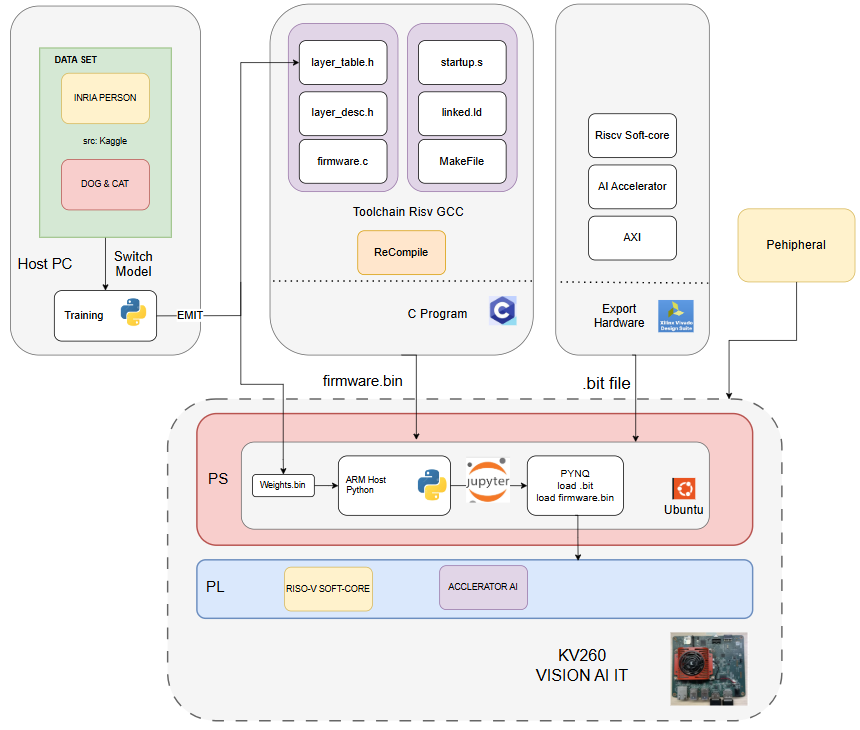
\includegraphics[width=1\linewidth]{chapter05/img/flowwork.png}
%     \caption{Sơ đồ tổng quan luồng dữ liệu giữa 4 tầng kiến trúc.}
%     \label{fig:flowwork}
% \end{figure}
% TODO: thêm hình flowwork.png khi vẽ xong block diagram 4-layer

\textbf{Quy ước giao tiếp giữa các tầng}
% Bảng artifacts (5 files)
\begin{table}[!h]
    \centering
    \caption{Các artifact trao đổi giữa các tầng trong pipeline.}
    \label{tab:artifacts}
    \begin{tabular}{|l|l|l|}
        \hline
        \textbf{Artifact} & \textbf{Sinh bởi} & \textbf{Tiêu thụ bởi} \\
        \hline
        \texttt{firmware.bin}    & RISC-V toolchain      & ARM (load vào I-BRAM)         \\
        \texttt{weights.bin}     & \texttt{train.ipynb}  & ARM (load vào DDR)            \\
        \texttt{meta.json}       & \texttt{train.ipynb}  & ARM (input quantization)      \\
        \texttt{layer\_table.h}  & \texttt{train.ipynb}  & RISC-V firmware (compile-in)  \\
        \texttt{bitstream.bit}   & Vivado synth+impl     & PYNQ Overlay                  \\
        \hline
    \end{tabular}
\end{table}

\newpage
\section{Huấn luyện và lượng tử hóa mô hình AI}
\label{sec:training_impl}

Pipeline huấn luyện được hiện thực dưới dạng một Jupyter notebook duy nhất \texttt{training/train.ipynb}, có khả năng chạy đồng thời trên Google Colab (sử dụng GPU miễn phí) và máy tính cá nhân (VSCode + Jupyter kernel). Notebook tự động phát hiện môi trường (Colab vs. local) ở cell đầu tiên và clone mã nguồn từ GitHub nếu chạy trên Colab.

\subsection{Cấu trúc pipeline 8 giai đoạn}
Notebook được tổ chức thành 8 phần (sections) tuần tự, người dùng chỉ cần chỉnh tham số ở phần ``Hyperparameters'' rồi nhấn ``Run All'' để nhận đầy đủ artifact xuất ra:

\begin{enumerate}
    \item \textbf{Environment} -- detect Colab/local, cài đặt thư viện (\texttt{tensorflow}, \texttt{kagglehub}).
    \item \textbf{Config} -- đặt \texttt{MODEL}, \texttt{DATASET}, \texttt{EPOCHS}, \texttt{BATCH\_SIZE}.
    \item \textbf{Dataset} -- tải dataset qua \texttt{kagglehub}, build pipeline \texttt{tf.data} (resize, normalize, cache, prefetch).
    \item \textbf{Model} -- khởi tạo \texttt{vgg-tiny} (hoặc các model legacy như VGG16, ResNet18 cho mục đích so sánh).
    \item \textbf{Train} -- compile + fit với Adam optimizer, sparse categorical crossentropy.
    \item \textbf{PTQ} -- chuyển mô hình FP32 sang INT8 thông qua \texttt{TFLiteConverter} với 100 batch hiệu chuẩn (\texttt{representative\_dataset}) lấy từ tập validation.
    \item \textbf{Emit} -- parse mô hình \texttt{.tflite}, sinh \texttt{layer\_table.h} (mảng C struct) và \texttt{weights.bin} (binary blob) trong thư mục \texttt{training/export/}.
    \item \textbf{Distribute} -- đóng gói artifact thành ZIP để tải xuống và \texttt{rsync} lên board KV260.
\end{enumerate}

\subsection{Kiến trúc \texttt{vgg-tiny} đề xuất}
Mô hình \texttt{vgg-tiny} là một mạng \textit{fully-convolutional} gồm 5 lớp Conv $3 \times 3$ stride-1 với padding VALID, sử dụng nguyên tắc đơn giản hóa để tránh các op chưa được bộ tăng tốc Conv-CNN v2.0 hỗ trợ (như Pool, Dense, Depthwise). Bảng~\ref{tab:vgg_tiny_layers} đã trình bày chi tiết kiến trúc trong chương~\ref{chp:04}.

\begin{lstlisting}[language=Python, caption={Kiến trúc Tiny-VGG đề xuất (file \texttt{edge\_train/models.py}).}]
def build_vgg_tiny(num_classes, input_shape=(128,128,3)):
    inp = tf.keras.Input(shape=input_shape)
    x = layers.Conv2D(8,  3, activation='relu', padding='valid')(inp)
    x = layers.Conv2D(16, 3, activation='relu', padding='valid')(x)
    x = layers.Conv2D(32, 3, activation='relu', padding='valid')(x)
    x = layers.Conv2D(64, 3, activation='relu', padding='valid')(x)
    x = layers.Conv2D(num_classes, 3, activation=None, padding='valid')(x)
    x = layers.GlobalAveragePooling2D()(x)
    return tf.keras.Model(inp, layers.Softmax()(x), name='vgg-tiny')
\end{lstlisting}

\subsection{Lượng tử hóa sau huấn luyện (Post-Training Quantization)}
Quá trình PTQ áp dụng kỹ thuật \textit{Integer-Arithmetic-Only Inference} của Jacob et al. \cite{jacob2018quantization} (đã trình bày tại mục~\ref{sec:quantization_theory}). Cụ thể trong notebook:

\begin{itemize}
    \item Sau khi mô hình FP32 đạt độ chính xác mục tiêu, \texttt{tf.lite.TFLiteConverter} được khởi tạo với \texttt{optimizations = [DEFAULT]}.
    \item Tham số \texttt{representative\_dataset} được gán bằng một generator lấy 100 batch từ tập validation -- đây là bước \textit{calibration} để xác định dải $[\min, \max]$ của activations cho từng layer.
    \item Tham số \texttt{inference\_input\_type} và \texttt{inference\_output\_type} đặt là \texttt{INT8} để buộc TFLite quantize cả input/output, giúp giảm bước dequantize ở runtime.
    \item Sau khi \texttt{convert()}, file \texttt{.tflite} thu được chứa đầy đủ trọng số INT8, scale và zero-point per-tensor cho từng layer.
\end{itemize}

\subsection{Trình biên dịch tự sinh \texttt{layer\_table.h} và \texttt{weights.bin}}
\label{ssec:emitter}
Module \texttt{edge\_train/emit.py} thực hiện vai trò ``compiler'' bằng cách parse mô hình \texttt{.tflite} (sử dụng FlatBuffer schema chính thức của TensorFlow Lite) và sinh hai artifact đồng bộ:

\begin{itemize}
    \item \textbf{\texttt{layer\_table.h}} -- mảng \texttt{layer\_desc\_t LAYERS[NUM\_LAYERS]} dưới dạng C header. Mỗi entry chứa: kích thước IFM (\texttt{w\_in}, \texttt{h\_in}), số kênh (\texttt{cin}, \texttt{cout}), offset trong \texttt{weights.bin}, hệ số $M_{q31}$ và $n$, zero-point đầu ra, cờ \texttt{has\_relu}. Tổng cộng 40 byte/layer.
    \item \textbf{\texttt{weights.bin}} -- binary blob chứa toàn bộ trọng số INT8 và bias INT32 nối tiếp nhau theo thứ tự layer. ARM tải file này vào DDR và RISC-V dùng \texttt{LAYERS[i].weight\_offset} để truy cập đúng vị trí cho từng layer.
\end{itemize}

Hàm \texttt{quantize\_multiplier()} chuyển hệ số nhân float $M = (s_{\mathrm{in}} \cdot s_{\mathrm{w}})/s_{\mathrm{out}}$ sang dạng cố định Q31 + dịch phải:
\begin{equation}
    M_{q31}, n = \texttt{quantize\_multiplier}\!\left(\frac{s_{\mathrm{in}} \cdot s_{\mathrm{w}}}{s_{\mathrm{out}}}\right)
\end{equation}
Hàm sử dụng \texttt{math.frexp()} của Python để tách $M$ thành significand và exponent, từ đó có $M_{q31} = \mathrm{round}(\text{significand} \cdot 2^{31})$ và $n = -\text{exponent}$. Trường hợp $M \geq 1$ (chưa được hỗ trợ bởi RTL hiện tại) sẽ được clip về giá trị max và in cảnh báo.

\newpage
\section{Hiện thực khối gia tốc phần cứng Conv\_CNN v2.0}
\label{sec:cnn-ip}

Bộ tăng tốc \texttt{conv\_cnn} v2.0 được hiện thực hóa dưới dạng một IP core độc lập trong Vivado IP Repository (\texttt{hw/ip\_repo/conv\_cnn\_1\_0}), với 3 giao diện AXI: \texttt{S00\_AXI} (control AXI4-Lite), \texttt{S00\_AXIS} (input stream cho IFM/weights), \texttt{M00\_AXIS} (output stream cho OFM). IP được thiết kế lại hoàn toàn từ phiên bản v1.x (Sobel-only, hardcode trọng số) thành kiến trúc tổng quát hỗ trợ Conv $3 \times 3$ INT8 đầy đủ với requantize TFLite.

\subsection{Tổng quan kiến trúc Conv\_CNN v2.0}
% Datapath block diagram
\begin{figure}[!h]
    \centering
    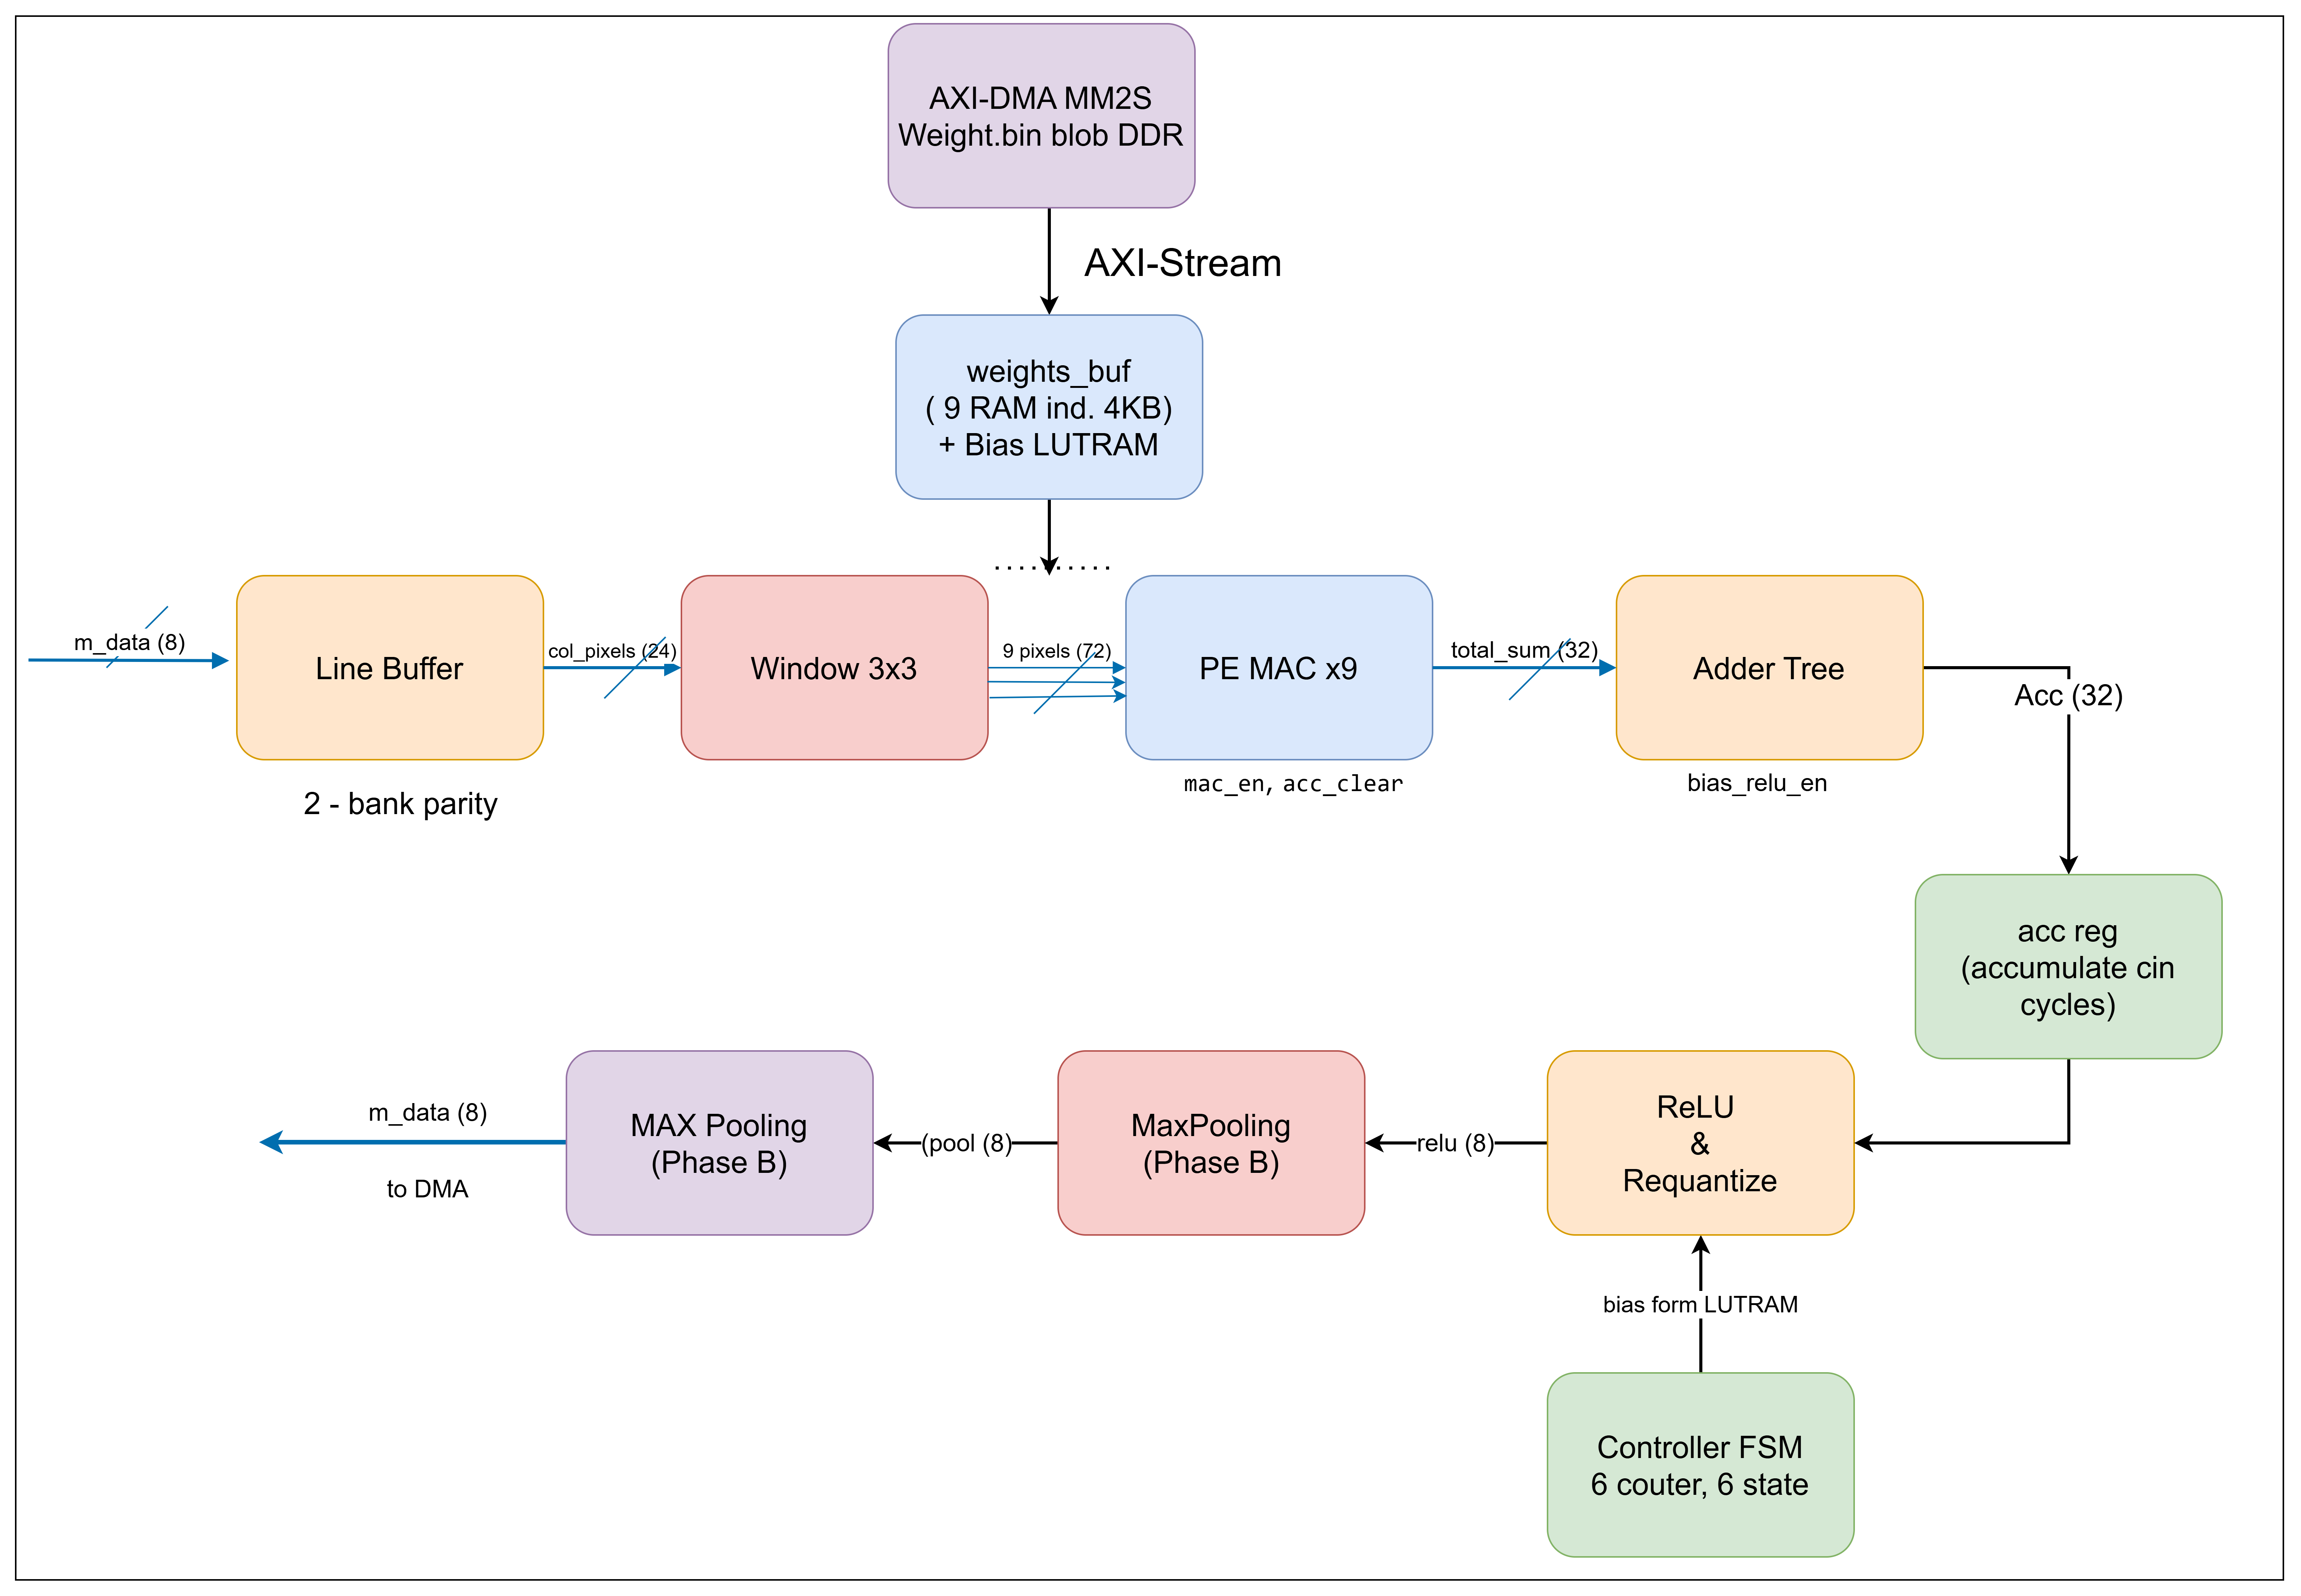
\includegraphics[width=1\textwidth]{chapter05/img/conv_cnn_datapath.png}
    \caption{Sơ đồ datapath conv\_cnn IP: từ AXIS in qua line buffer,
    window, MAC array, requantize đến AXIS out.}
    \label{fig:conv-cnn-datapath}
\end{figure}

Datapath gồm 7 module chính phối hợp qua một FSM trung tâm:
\begin{itemize}
    \item \texttt{conv\_pkg.sv} -- package tham số (giới hạn kích thước, độ rộng datatype, độ trễ pipeline).
    \item \texttt{controller\_fsm.sv} -- FSM 6 trạng thái, 6 bộ đếm điều phối luồng kênh-xen-kẽ và iteration trên \texttt{cnt\_cout}.
    \item \texttt{line\_buffer.sv} -- 2 bank BRAM cho 2 hàng pixel cũ, ping-pong theo parity hàng.
    \item \texttt{window\_3x3.sv} -- mảng thanh ghi $3 \times 3 \times \texttt{MAX\_CIN}$ giữ cửa sổ tích chập hiện tại.
    \item \texttt{weight\_buf.sv} -- 9 BRAM độc lập cho weights + LUTRAM cho bias INT32.
    \item \texttt{pe\_mac.sv} -- 9 PE MAC INT8$\times$INT8 song song (DSP48E2-mappable).
    \item \texttt{requantize.sv} -- pipeline 3-tầng: cộng bias, nhân $M_{q31}$, dịch phải, cộng zero-point, bão hòa, ReLU.
\end{itemize}

\subsection{Tham số hóa và package \texttt{conv\_pkg.sv}}
Toàn bộ tham số bound (\texttt{MAX\_WIDTH}, \texttt{MAX\_CIN}, \texttt{MAX\_COUT}) và độ rộng datatype được đặt trong \texttt{conv\_pkg.sv}, cho phép scale tài nguyên mà không sửa từng module. Phiên bản hiện tại đặt \texttt{MAX\_WIDTH = 128}, \texttt{MAX\_CIN = MAX\_COUT = 64} -- vừa đủ cho \texttt{vgg-tiny} mà không phình tài nguyên không cần thiết. Việc đẩy lên cho mạng lớn hơn (như VGG11) chỉ cần thay tham số trong package và re-synthesize.

\subsection{Khối điều khiển \texttt{controller\_fsm.sv}}
FSM gồm 6 trạng thái (\texttt{S\_IDLE}, \texttt{S\_ACCEPT\_CIN}, \texttt{S\_LATCH\_WIN}, \texttt{S\_COMPUTE}, \texttt{S\_WAIT\_REQUANT}, \texttt{S\_EMIT}) phối hợp với 6 bộ đếm để duyệt 3 vòng lặp lồng nhau:

\begin{lstlisting}[language=Verilog, caption={Trình tự duyệt 3 vòng lặp trong controller FSM}, label={lst:fsm}]
for (y_in, x_in raster scan):                  // outer
    for (cin in 0..num_cin-1): receive 1 IFM    // channel-interleaved
    if (window valid):
        for (cnt_cout in 0..num_cout-1):        // middle
            mac_clear; for (cnt_cin in 0..num_cin-1) mac_enable
            requant_in_valid -> wait latency -> emit M_AXIS
\end{lstlisting}

Cơ chế \textit{channel-interleaved per pixel} cho phép pipeline IFM input liên tục: tại mỗi vị trí pixel, FSM nhận \texttt{num\_cin} samples (một sample/cycle) trước khi cửa sổ trượt qua vị trí kế. Số chu kỳ tính toán cho mỗi pixel output xấp xỉ $\texttt{num\_cout} \times (\texttt{num\_cin} + L_{\mathrm{requant}} + 1)$.

\subsection{Bộ đệm dòng và cửa sổ \texttt{line\_buffer.sv}, \texttt{window\_3x3.sv}}
Để thực hiện tích chập $3 \times 3$, tại mỗi thời điểm cần 3 hàng pixel liên tiếp cùng lúc. Module \texttt{line\_buffer.sv} sử dụng \textbf{2 bank BRAM} mỗi bank dung lượng $\texttt{MAX\_W} \times \texttt{MAX\_CIN}$ byte với cơ chế \textit{read-before-write parity-toggled}: khi pixel mới ghi vào bank này thì hai hàng cũ vẫn được giữ ở bank kia, tránh ghi đè dữ liệu đang đọc. Độ trễ đọc BRAM 1 chu kỳ được FSM bù trừ bằng pipeline alignment register.

Module \texttt{window\_3x3.sv} là một mảng thanh ghi $3 \times 3 \times \texttt{MAX\_CIN}$, dịch cột mỗi khi tín hiệu \texttt{shift\_cols} được nhả. Khi cần đọc 9 pixel cho một kênh \texttt{cnt\_cin} cụ thể, mảng cung cấp đầu ra tổ hợp ngay trong chu kỳ đó (không có thanh ghi đầu ra), giảm độ trễ tính toán.

\subsection{Bộ nhớ trọng số \texttt{weight\_buf.sv} -- bài học về BRAM inference}
\label{ssec:weight_buf_bram}
Một trong những vấn đề nan giải trong quá trình hiện thực hóa là Vivado synth không suy luận đúng BRAM cho mảng trọng số. Phiên bản đầu tiên sử dụng mảng 3D unpacked \texttt{[K\_TAPS][MAX\_COUT][MAX\_CIN]} với reset đồng bộ, dẫn đến tổng hợp ra \textbf{295,000 FFs} (FDRE -- thanh ghi flip-flop) thay vì BRAM, vượt xa tài nguyên FPGA cho phép.

Sau khi tách thành \textbf{9 mảng 2D độc lập} (mỗi mảng tương ứng 1 trong 9 vị trí kernel) và bỏ lệnh reset đồng bộ, Vivado mới suy luận đúng thành \textbf{9 RAMB18 / 4 KB mỗi block}, tổng 36 KB. Bias INT32 lưu trong LUTRAM (do số lượng nhỏ -- tối đa 64 entry). Đây là một trong những bài học kỹ thuật quan trọng được rút ra: cấu trúc dữ liệu trong RTL có ảnh hưởng quyết định đến việc Vivado suy luận BRAM hay FF -- và sự khác biệt về tài nguyên có thể lên đến vài bậc độ lớn.

Cơ chế nạp weights theo từng layer được điều khiển bởi cờ \texttt{mode\_load} trong thanh ghi \texttt{CTRL}: khi \texttt{mode\_load = 1}, FSM chuyển sang trạng thái nhận stream từ \texttt{S00\_AXIS} và ghi tuần tự vào 9 BRAM + LUTRAM bias. Khi nạp xong, RISC-V đặt \texttt{mode\_load = 0} và bắt đầu chế độ infer.

\subsection{Mảng MAC và cây cộng \texttt{pe\_mac.sv}}
Mỗi PE thực hiện $a_{\mathrm{int8}} \times w_{\mathrm{int8}} \to \mathrm{int32}$ rồi cộng vào thanh ghi tích lũy 32-bit. Cấu trúc với 2 thanh ghi pipeline (MREG sau nhân, PREG sau cộng) cho phép Vivado ánh xạ trực tiếp vào DSP48E2 với 1 DSP/PE. 9 PE chạy song song xử lý đồng thời 9 vị trí của kernel $3 \times 3$, đầu ra được tổng hợp qua \textit{adder tree} 4-tầng (combinational) để cho ra một giá trị tích chập 32-bit/cycle.

Đối với mạng có \texttt{cin > 1}, kết quả của 9 PE được tích lũy thêm qua \texttt{cin} chu kỳ trong thanh ghi \texttt{acc[31:0]} trước khi xuất sang khối requantize. Tổng cộng cần $9 \times \texttt{cin}$ phép nhân INT8 cho mỗi điểm OFM.

\subsection{Khối lượng tử hóa lại \texttt{requantize.sv}}
\label{ssec:requantize}
Khối requantize hiện thực công thức TFLite \cite{jacob2018quantization}:
\begin{equation}
    y_{q} = \mathrm{sat}_{\mathrm{INT8}}\!\left(
        \left\lfloor \frac{(\sum_{i,j,c} x \cdot w + b) \cdot M_{q31} + 2^{30+n}}{2^{31+n}} \right\rfloor + z_{\mathrm{out}}
    \right)
\end{equation}

Pipeline 3-tầng:
\begin{itemize}
    \item \textbf{Tầng 1 -- bias add:} cộng bias INT32 (đọc từ LUTRAM) với accumulator 32-bit.
    \item \textbf{Tầng 2 -- multiply $M_{q31}$:} nhân INT32 $\times$ INT31 thành INT63, có làm tròn round-half-up (cộng $2^{30+n}$ trước khi dịch).
    \item \textbf{Tầng 3 -- shift + zero-point + saturate + ReLU:} dịch phải $31 + n$ bit qua barrel shifter, cộng zero-point INT8, bão hòa về dải $[-128, 127]$, kẹp về $[0, 127]$ nếu \texttt{has\_relu = 1}.
\end{itemize}

\subsection{Tích hợp tổng thể qua AXI}
% S00_AXI register map (Bảng 5.x)
% AXI-Stream IFM/OFM
\begin{table}[htbp]
    \centering
    \caption{Bản đồ thanh ghi điều khiển S00\_AXI (32 bytes, 8 thanh ghi).}
    \label{tab:s00-axi-regs}
    \begin{tabular}{|c|l|c|l|}
        \hline
        \textbf{Offset} & \textbf{Tên} & \textbf{R/W} & \textbf{Layout} \\
        \hline
        0x00 & GEOMETRY  & RW & width[15:0], height[31:16] \\
        0x04 & CTRL      & RW & start, pool\_en, mode\_load, has\_relu \\
        0x08 & STATUS    & RO & done \\
        0x0C & CHANNELS  & RW & num\_cin[15:0], num\_cout[31:16] \\
        0x10 & M\_Q31    & RW & Q31 multiplier \\
        0x14 & SHIFT\_ZP & RW & shift[5:0], output\_zp[15:8] \\
        \hline
    \end{tabular}
\end{table}

Trình tự lập trình một layer (do firmware RISC-V thực hiện trong \texttt{process\_one\_layer()}):
\begin{enumerate}
    \item Ghi \texttt{GEOMETRY}, \texttt{CHANNELS}, \texttt{M\_Q31}, \texttt{SHIFT\_ZP} cho layer hiện tại.
    \item Ghi \texttt{CTRL.mode\_load = 1, CTRL.start = 1} (load mode), DMA stream weights tới \texttt{S00\_AXIS}, poll \texttt{STATUS.done}.
    \item Đặt \texttt{CTRL.has\_relu, CTRL.start = 1} (infer mode), DMA stream IFM tới \texttt{S00\_AXIS}, OFM được M00\_AXIS đẩy về DDR qua S2MM.
    \item Poll \texttt{STATUS.done = 1}, hạ \texttt{CTRL.start = 0}, chuyển sang layer tiếp theo.
\end{enumerate}

\subsection{Đánh giá khối tăng tốc CONV-CNN}

\begin{figure}[!h]
    \centering
    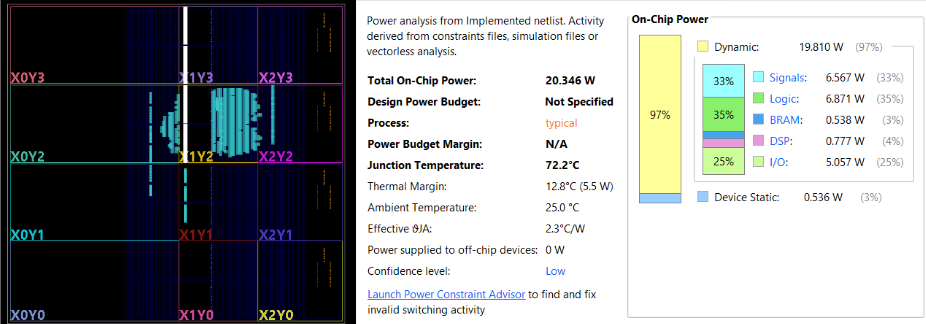
\includegraphics[width=1\linewidth]{chapter05/img/cnn_imple.png}
    \caption{Báo cáo chạy khối CNN}
    \label{fig:overall}
\end{figure}

\begin{figure}[!h]
    \centering
    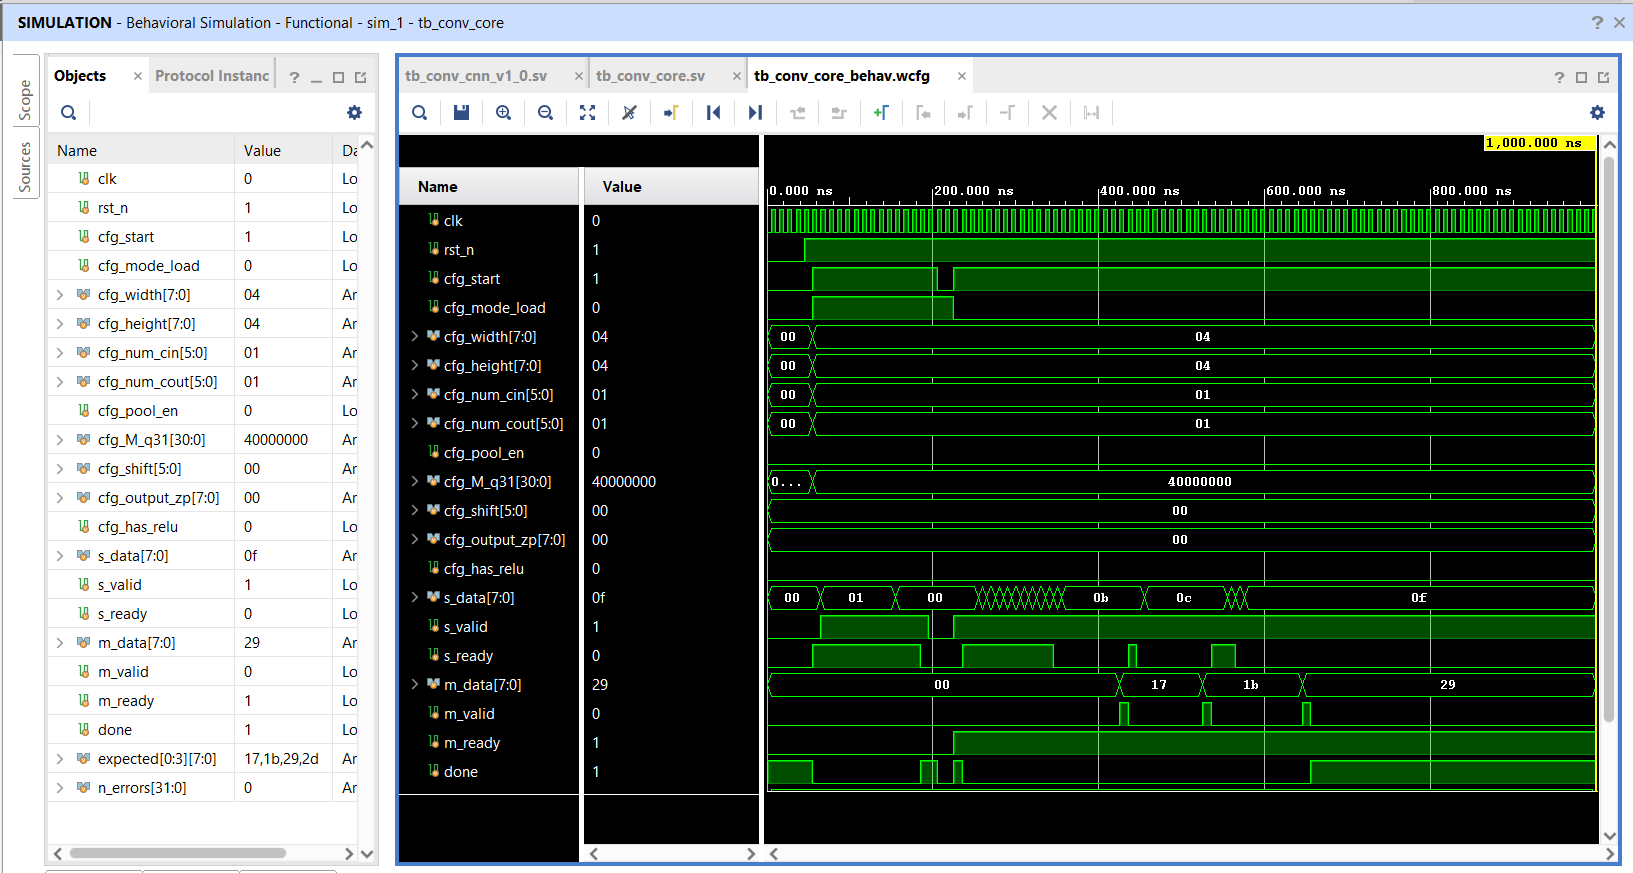
\includegraphics[width=1\linewidth]{chapter05/img/cnn_waveform.png}
    \caption{Kết quả chạy simulate khối CNN}
    \label{fig:waveform}
\end{figure}

\newpage
\section{Hiện thực RISC-V Soft-core}
\subsection{Tinh chỉnh CV32E40P Core}
Lõi vi xử lý CV32E40P mã nguồn mở nguyên bản được thiết kế với đầy đủ các tập lệnh mở rộng, bao gồm cả khối xử lý số thực dấu phẩy động (FPU - Floating Point Unit). Tuy nhiên, để tối ưu hóa tài nguyên phần cứng (LUT, FF, DSP) trên chip FPGA cho bộ tăng tốc trí tuệ nhân tạo, lõi CPU đã được tinh chỉnh lại ở mức mã nguồn RTL.

Cụ thể, toàn bộ khối xử lý số thực và các lệnh liên quan (tập lệnh mở rộng F) đã được loại bỏ. Sự tinh giản này là hoàn toàn hợp lý do toàn bộ mô hình học sâu trong hệ thống đã được lượng tử hóa xuống kiểu dữ liệu số nguyên 8-bit (INT8). Vi xử lý lúc này chỉ hoạt động với tập lệnh cơ bản RV32IMC, chịu trách nhiệm điều phối luồng điều khiển, quản lý ngắt và cấu hình thanh ghi thay vì tham gia tính toán trực tiếp. Bên cạnh đó, bộ giải mã lệnh (Instruction Decoder) cũng được tùy biến để tối ưu hóa đường truyền dữ liệu, loại bỏ các khối logic không cần thiết, giúp cải thiện tần số hoạt động tối đa (Fmax) của lõi.

\subsection{Hiện thực cầu nối giao tiếp OBI sang AXI4 (OBI to AXI)}
\label{sec:obi_axi}
Giao thức giao tiếp bộ nhớ mặc định của lõi CV32E40P là OBI (Open Bus Interface). Tuy nhiên, nền tảng thiết kế SoC của Xilinx Vivado sử dụng chuẩn giao tiếp AMBA AXI4 làm nòng cốt. Để tích hợp thành công lõi RISC-V vào bản vẽ hệ thống cùng với khối xử lý trung tâm (PS) và các bộ nhớ đệm, một cầu nối giao tiếp (Bridge) chuyển đổi từ tín hiệu OBI sang AXI4 đã được thiết kế và hiện thực.

Cầu nối này (\texttt{obi\_to\_axi.sv}) bao gồm hai luồng độc lập: một luồng dành cho việc nạp lệnh (Instruction Fetch) và một luồng dành cho truy xuất dữ liệu (Data Access). Khối logic bên trong sử dụng \texttt{fifo\_v3} để theo dõi các giao dịch outstanding (\texttt{MaxRequests = 4}), thực hiện nhiệm vụ biên dịch các tín hiệu điều khiển OBI (\textit{req}, \textit{gnt}, \textit{rvalid}) thành các kênh AXI4-Lite tương ứng (AR, R, AW, W, B). Quá trình kiểm thử mô phỏng (\texttt{tb\_riscv\_top.sv}) xác nhận cầu nối không gây ra trạng thái tắc nghẽn (Deadlock) và xử lý chính xác cả các tín hiệu báo lỗi đường truyền.

\subsection{Đóng gói IP \texttt{riscv\_top}}
Toàn bộ wrapper \texttt{riscv\_top.sv} (gồm CV32E40P + 2 instance \texttt{obi\_to\_axi}) được đóng gói thành Vivado IP \texttt{hw/ip\_repo/riscv\_top\_1\_0} với 3 cổng external bổ sung:
\begin{itemize}
    \item \texttt{fetch\_enable\_i} -- ARM điều khiển boot/halt qua AXI GPIO.
    \item \texttt{irq\_conv\_cnn\_i} -- ngắt level từ \texttt{conv\_cnn.irq} được map vào MFAST0 (\texttt{mip[16]}).
    \item \texttt{core\_sleep\_o} -- trạng thái WFI để ARM poll.
\end{itemize}

\newpage
\section{Hiện thực Firmware RISC-V (Layer 2 -- Orchestrator)}
\label{sec:firmware}

Firmware RISC-V được viết bằng ngôn ngữ C bare-metal (không có hệ điều hành), biên dịch bằng \texttt{riscv-none-elf-gcc} với cờ \texttt{-march=rv32imc -mabi=ilp32}. Toàn bộ \texttt{.text + .rodata} (bao gồm \texttt{LAYERS[]} từ \texttt{layer\_table.h}) được nạp vào I-BRAM 64 KB, còn \texttt{.data + .bss + stack} nằm ở D-BRAM 256 KB.

\subsection{Tổ chức bộ nhớ -- linker script}
File \texttt{linked.ld} định nghĩa hai vùng nhớ split:

\begin{lstlisting}[language=C, caption={Trích đoạn linker script \texttt{firmware/linked.ld}.}]
MEMORY {
    IRAM (rx)  : ORIGIN = 0x00000000, LENGTH = 64K  /* I-BRAM: .text, .rodata */
    DRAM (rwx) : ORIGIN = 0xB0040000, LENGTH = 256K /* D-BRAM: .data, .bss, stack */
}
\end{lstlisting}

Stack được khởi tạo tại \texttt{ORIGIN(DRAM) + LENGTH(DRAM) = 0xB008\_0000} bởi \texttt{startup.s} -- file assembly chứa reset handler: thiết lập \texttt{sp}, zero-out \texttt{.bss}, sao chép \texttt{.data} từ ROM (nếu có) và nhảy đến \texttt{main()}.

\subsection{Vòng đời driver \texttt{main.c}}
Hàm \texttt{main()} chạy theo polling loop đơn giản (chế độ ngắt được dành cho phiên bản tối ưu sau):

\begin{lstlisting}[language=C, caption={Polling loop chính của firmware.}]
int main(void) {
    while (1) {
        if (mmio_r32(REG_CMD_FROM_ARM) == CMD_START) {
            mmio_w32(REG_STATUS_TO_ARM, STATUS_BUSY);
            uint32_t base_w = mmio_r32(REG_WEIGHT_BASE);
            uint32_t buf_a  = mmio_r32(REG_IFM_PHYS_ADDR);
            uint32_t buf_b  = mmio_r32(REG_OFM_PHYS_ADDR);
            for (int i = 0; i < NUM_LAYERS; i++) {
                uint32_t in  = (i & 1) ? buf_b : buf_a;
                uint32_t out = (i & 1) ? buf_a : buf_b;
                process_one_layer(&LAYERS[i], base_w, in, out);
            }
            mmio_w32(REG_STATUS_TO_ARM, STATUS_DONE);
            mmio_w32(REG_CMD_FROM_ARM, CMD_IDLE);
        }
    }
}
\end{lstlisting}

Hàm \texttt{process\_one\_layer()} thực hiện đầy đủ trình tự 4 bước (mục~\ref{sec:cnn-ip}): nạp weights qua DMA, lập trình DMA cho IFM/OFM, kích hoạt conv\_cnn ở chế độ infer, và poll \texttt{STATUS.done}. Ping-pong DDR giữa \texttt{buf\_a} và \texttt{buf\_b} đảm bảo OFM của layer $i$ được làm IFM cho layer $i+1$ mà không cần phân bổ buffer riêng.

\newpage
\section{Hiện thực Host Runtime (Layer 3 -- PYNQ Application)}
\label{sec:host_runtime}

Tầng ứng dụng chạy trên ARM Cortex-A53 dưới Ubuntu PYNQ Image (Kria-PYNQ v3.0), sử dụng thư viện PYNQ để tải bitstream, cấp phát buffer DDR cache-coherent (CMA) và viết MMIO. Mã nguồn được tổ chức thành package \texttt{host/edge\_ai/} (4 module ngắn) phục vụ cả notebook lẫn CLI.

\subsection{Cấu trúc package \texttt{host/edge\_ai/}}
\begin{itemize}
    \item \texttt{constants.py} -- bản đồ thanh ghi (\texttt{REG\_*}), cờ trạng thái (\texttt{STATUS\_*}, \texttt{CMD\_*}), tên IP BRAM. \textbf{Phải đồng bộ với \texttt{firmware/main.c}}.
    \item \texttt{overlay.py} -- class \texttt{EdgeAIOverlay} bọc \texttt{pynq.Overlay}, cung cấp các method \texttt{load\_firmware()}, \texttt{kick()}, \texttt{poll\_done(timeout)}, \texttt{set\_io\_buffers(buf\_a, buf\_b)}.
    \item \texttt{preprocess.py} -- \texttt{cv2.imread} $\to$ resize $128 \times 128$ $\to$ INT8 quantize (đọc \texttt{input\_scale}, \texttt{input\_zero\_point} từ \texttt{meta.json}).
    \item \texttt{postprocess.py} -- Global Average Pool trên trục $(H, W)$ + dequantize float + softmax + argmax.
\end{itemize}

\subsection{Quy trình tải bitstream và boot RISC-V}
\begin{lstlisting}[language=Python, caption={Trình tự khởi động hệ thống trong notebook (rút gọn).}]
from edge_ai.overlay import EdgeAIOverlay
ov = EdgeAIOverlay("kria_soc_wrapper.bit")  # auto-loads .hwh

# Reset RISC-V, nap firmware vao I-BRAM, release reset
ov.load_firmware("firmware.bin")             # axi_bram_ctrl_2 Port B
ov.release_riscv_reset()                     # axi_gpio fetch_enable_i = 1

# Cap phat 3 buffer DDR cache-coherent (CMA)
import pynq, numpy as np
wbuf  = pynq.allocate(shape=(WEIGHTS_SIZE,),  dtype=np.int8)
buf_a = pynq.allocate(shape=(MAX_OFM_BYTES,), dtype=np.int8)
buf_b = pynq.allocate(shape=(MAX_OFM_BYTES,), dtype=np.int8)

# Nap weights.bin va publish dia chi vat ly cho RISC-V
wbuf[:] = np.fromfile("vgg-tiny_cats_dogs.weights.bin", dtype=np.int8)
wbuf.flush()
ov.set_weights_addr(wbuf.physical_address)
ov.set_io_buffers(buf_a.physical_address, buf_b.physical_address)
\end{lstlisting}

\subsection{Inference loop trong notebook}
Sau khi setup xong, phần lặp thực thi cho mỗi ảnh (cell ``2.3 DMA + kick + poll'' trong \texttt{inference\_demo.ipynb}):

\begin{enumerate}
    \item \texttt{img\_q = preprocess\_image(path, meta)} -- đọc + resize + quantize INT8.
    \item \texttt{buf\_a[:] = img\_q.flatten(); buf\_a.flush()} -- ghi IFM vào CMA buffer.
    \item \texttt{ov.kick()} -- ghi \texttt{CMD\_START} qua MMIO, RISC-V phát hiện và bắt đầu duyệt LAYERS[].
    \item \texttt{ov.poll\_done(timeout=2.0)} -- chờ \texttt{STATUS\_TO\_ARM == STATUS\_DONE}.
    \item Đọc OFM cuối từ \texttt{buf\_a} hoặc \texttt{buf\_b} (xác định bởi \texttt{meta['fpga']['final\_ofm\_buf\_idx']}), gọi \texttt{.invalidate()} trước khi đọc.
    \item \texttt{cls, conf = postprocess.gap\_argmax(ofm, scale, zp)} -- GAP $\to$ softmax $\to$ argmax.
\end{enumerate}

Notebook \texttt{benchmark.ipynb} bổ sung sweep accuracy + latency trên toàn tập validation, vẽ confusion matrix và histogram độ trễ để đánh giá hiệu năng end-to-end.

\newpage
\section{Tích hợp Block Design trong Vivado}

\label{sec:bd}
\begin{figure}[H] % cần \usepackage{float}
\centering

\includegraphics[width=\linewidth]{chapter05/img/arch.png}
\caption{Sơ khối minh họa hệ thống}
\label{fig:arch}
\end{figure}


\begin{figure}[H]
\centering
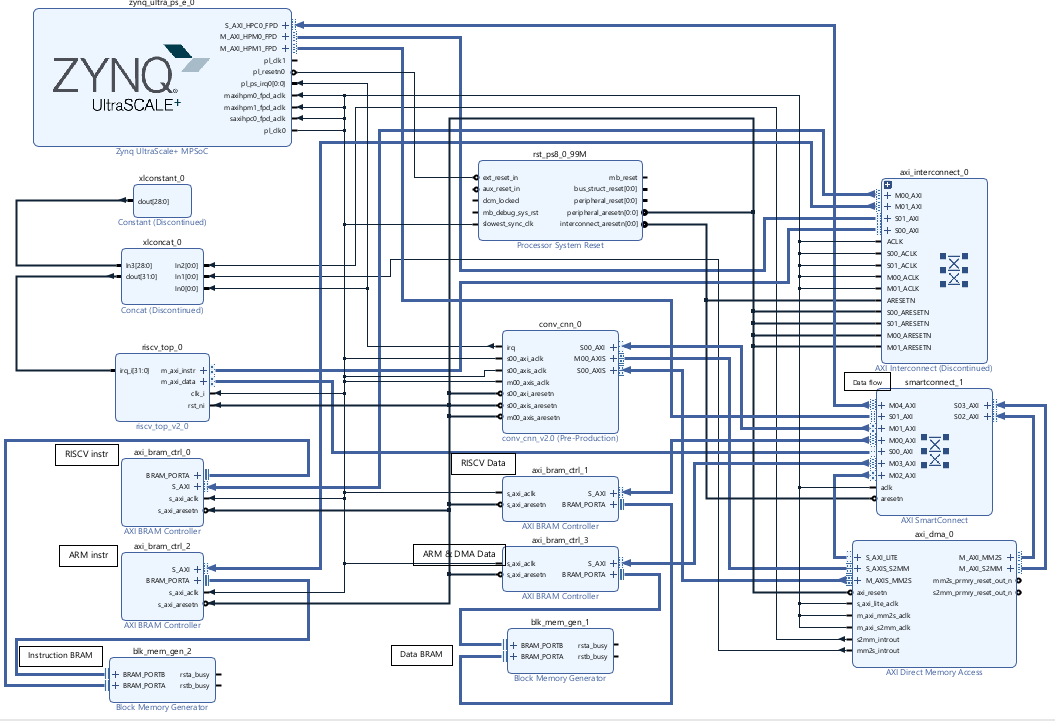
\includegraphics[width=1.2\linewidth, angle=90]{chapter05/img/arch_vivado.png}
\caption{Thiết kế khối trong vivado}
\label{fig:arch_vivado}
\end{figure}


\newpage
\subsection{Bản đồ bộ nhớ và Address Editor}
% RISC-V view, ARM view, DMA view
% BD validation issues đã giải quyết
\begin{figure}[h]
    \centering
    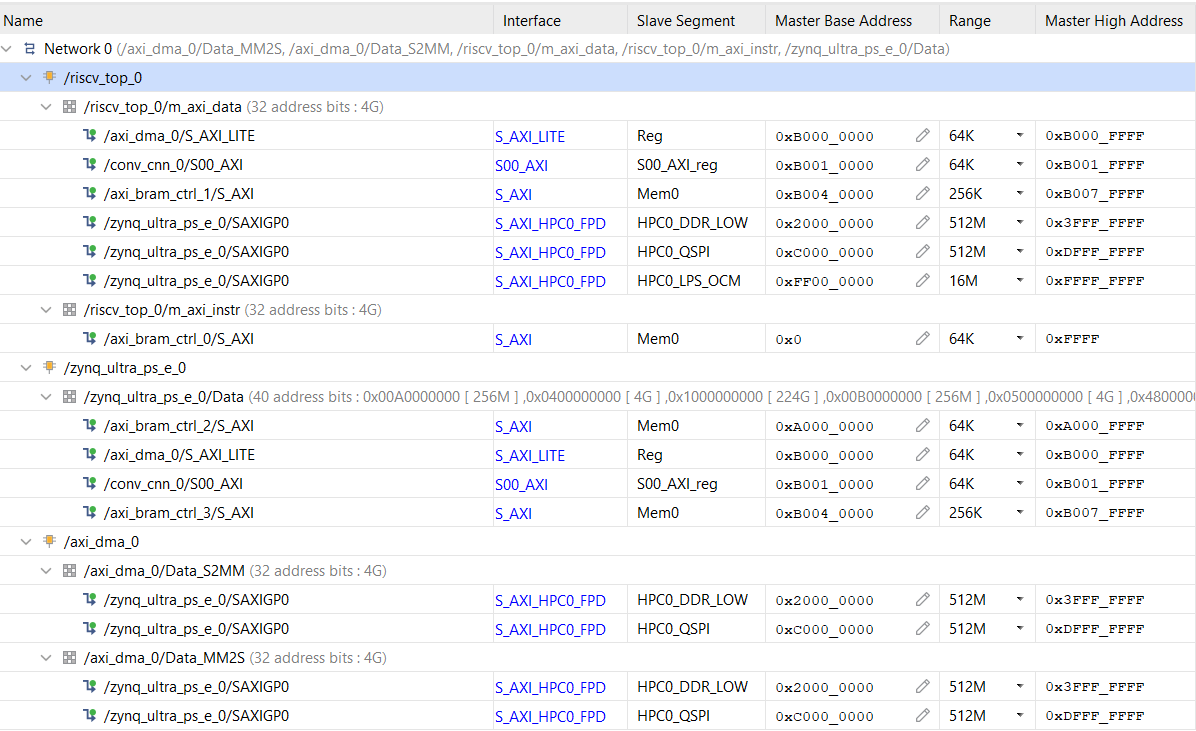
\includegraphics[width=1\linewidth]{chapter05//img/address_editor.png}
    \caption{Bảng chia section trong bộ nhớ}
    \label{fig:address_editor}
\end{figure}

Quá trình tích hợp Block Design ban đầu phát sinh 6 cảnh báo từ Vivado Address Editor (2 errors BD~41-1267 + 4 critical warnings) do SmartConnect mặc định mở route từ \texttt{axi\_dma\_0/Data\_MM2S/S2MM} đến \texttt{axi\_bram\_ctrl\_1} (D-BRAM Port A của RISC-V). Vấn đề được giải quyết bằng 3 thao tác trong Address Editor:

\begin{enumerate}
    \item Đồng bộ offset RISC-V $\leftrightarrow$ PS để cùng slave có cùng địa chỉ logic (cùng nằm trong dải \texttt{0xB0xx\_xxxx}).
    \item Exclude DMA $\to$ BRAM (DMA chỉ thấy DDR qua \texttt{S\_AXI\_HPC0\_FPD}, không thấy BRAM).
    \item Exclude RISC-V $\to$ \texttt{axi\_bram\_ctrl\_3} (RISC-V chỉ ghi Port A của D-BRAM, Port B dành riêng cho ARM).
\end{enumerate}

Sau khi fix, validate sạch (0 errors / 0 critical warnings), bitstream được tổng hợp thành công.

\newpage
\subsection{Đồng bộ ARM \(\leftrightarrow\) RISC-V qua D-BRAM dual-port}
% Bảng register layout shared region
Mặc dù D-BRAM 256~KB là một khối BRAM duy nhất ở mức vật lý, nó được cấu hình dual-port (RAMB36 trên Ultrascale+) với hai \texttt{axi\_bram\_ctrl} riêng biệt (Port A cho RISC-V, Port B cho ARM). Phần đầu của vùng nhớ này được dành cho các thanh ghi handshake (Bảng~\ref{tab:handshake-regs-ch5}), giúp ARM và RISC-V trao đổi command/status với độ trễ cực thấp (zero round-trip qua DDR).

\begin{table}[h]
    \centering
    \caption{Bố cục thanh ghi handshake D-BRAM Port B (offset từ \texttt{0xB004\_0000}).}
    \label{tab:handshake-regs-ch5}
    \begin{tabular}{|l|l|l|p{4.5cm}|}
        \hline
        \textbf{Offset} & \textbf{Tên} & \textbf{Hướng} & \textbf{Mô tả} \\ \hline
        +0x00 & \texttt{CMD\_FROM\_ARM}    & ARM $\to$ RISC-V & \texttt{0x01} = START \\ \hline
        +0x04 & \texttt{STATUS\_TO\_ARM}   & RISC-V $\to$ ARM & IDLE / BUSY / DONE \\ \hline
        +0x08 & \texttt{DATASET\_ID}       & ARM $\to$ RISC-V & 0 = INRIA, 1 = cats\_dogs \\ \hline
        +0x18 & \texttt{IFM\_PHYS\_ADDR}   & ARM $\to$ RISC-V & DDR addr buffer A \\ \hline
        +0x1C & \texttt{OFM\_PHYS\_ADDR}   & ARM $\to$ RISC-V & DDR addr buffer B \\ \hline
        +0x20 & \texttt{WEIGHT\_BASE}      & ARM $\to$ RISC-V & DDR addr weights blob \\ \hline
    \end{tabular}
\end{table}

\newpage
\section{Quy trình kiểm thử}
\label{sec:testing}

Hệ thống được kiểm thử theo phương pháp tiếp cận \textit{nhiều tầng} (multi-level testing) để cô lập lỗi sớm: từ unit testbench RTL $\to$ tích hợp IP $\to$ đối chiếu golden vector $\to$ kiểm thử end-to-end trên board.

\subsection{Kiểm thử đơn vị (Unit Testbench)}
% TB từng module: requantize, FSM, line_buffer
% Vector test thủ công
Mỗi module RTL chính có testbench riêng kiểm tra hành vi cô lập với input có chủ đích:
\begin{itemize}
    \item \texttt{tb\_requantize} -- vector hoá trị đầu vào dải $[-2^{20}, 2^{20}]$, đối chiếu với reference Python (Q31 mul + barrel shift) để xác nhận round-half-up đúng.
    \item \texttt{tb\_line\_buffer} -- ghi tuần tự một frame $128 \times 128$, kiểm tra parity-toggle giữ nguyên 2 hàng cũ khi hàng mới được ghi.
    \item \texttt{tb\_riscv\_top.sv} -- behavioral instr memory đáp NOP, kiểm tra fetch advance qua \texttt{m\_axi\_instr}.
\end{itemize}

\subsection{Kiểm thử tích hợp IP}
\label{ssec:tb-ip}
Testbench \texttt{tb\_conv\_core.sv} mô phỏng toàn bộ luồng load + infer
với input 4×4×1, weights toàn 1, M=0.5, kỳ vọng OFM = $\{23, 27, 41, 45\}$
(với round-half-up).

\begin{equation}
    y_{q} = \mathrm{sat}_{\mathrm{INT8}}\!\left(
        \left\lfloor \frac{(\sum_{i,j,c} x \cdot w + b) \cdot M_{q31} + 2^{30+n}}{2^{31+n}} \right\rfloor + z_{\mathrm{out}}
    \right)
\end{equation}

\subsection{Đối chiếu với golden vector từ TFLite Interpreter}
% Bit-exact comparison strategy
% Per-tensor vs per-axis quant note
Để đảm bảo tính đúng đắn của RTL trước khi kiểm thử trên board, mỗi layer của \texttt{vgg-tiny} được chạy song song bằng \texttt{tf.lite.Interpreter} (đã quantize INT8) trên Host PC. Đầu ra OFM của TFLite được lưu thành mảng INT8 và so sánh \textbf{bit-exact} với OFM mà testbench RTL sinh ra. Cách so sánh này hiệu quả vì TFLite cũng dùng đúng công thức Q31 multiplier với round-half-up, do đó không có sai số làm tròn giữa hai phía.

Một lưu ý kỹ thuật quan trọng: TFLite mặc định dùng \textit{per-axis quantization} cho weight (mỗi cout-channel có scale riêng), trong khi RTL hiện tại chỉ hỗ trợ \textit{per-tensor} (1 scale cho cả layer). Do đó pipeline emit phải force convert sang per-tensor (\texttt{disable\_per\_channel = True}) -- điều này gây giảm độ chính xác khoảng 0.5--2\% trên các layer sâu, là một đánh đổi đã được cân nhắc kỹ trong giai đoạn thiết kế.

\subsection{Kiểm thử trên board KV260}
% Hardware-in-the-loop methodology
% Dataset split (train/val/test)
Sau khi qua đủ các tầng kiểm thử mô phỏng, hệ thống được triển khai xuống board Kria KV260 thật:

\begin{itemize}
    \item \textbf{Triển khai:} Script \texttt{deploy.sh} sử dụng \texttt{rsync} để đồng bộ 4 nhánh artifact (\texttt{hw/artifacts/} -- bitstream + .hwh; \texttt{firmware/firmware.bin}; \texttt{training/export/} -- weights + meta.json; \texttt{host/} -- Python package + notebooks) từ PC sang board qua SSH.
    \item \textbf{Sanity check:} Chạy \texttt{inference\_demo.ipynb} với một ảnh test đơn lẻ, kiểm tra latency, và visual hóa kết quả classification.
    \item \textbf{Đánh giá hệ thống:} Chạy \texttt{benchmark.ipynb} qua toàn bộ tập validation, ghi nhận \textit{accuracy} và \textit{latency} cho mỗi ảnh.
    \item \textbf{Hardware-in-the-loop comparison:} Mỗi ảnh được chạy đồng thời qua (i) TFLite Interpreter trên ARM (reference), và (ii) Conv-CNN trên FPGA. Đầu ra logits được so sánh; sai khác nếu có thường < 1 LSB do thứ tự cộng dồn floating ở pipeline ARM.
\end{itemize}

Kết quả định lượng (accuracy, latency, sai số) được trình bày chi tiết tại chương~\ref{chp:06}.

\chapter{Kết quả}
\label{chp:06}

Trong chương này, nhóm thực hiện trình bày các kết quả đạt được của đồ án, bao gồm hai phần chính: Đánh giá quá trình tổng hợp phần cứng (Hardware Synthesis) trên phần mềm Xilinx Vivado và đánh giá hiệu năng huấn luyện, lượng tử hóa các mô hình Mạng nơ-ron tích chập (CNN) trước khi triển khai thực tế xuống bo mạch Kria KV260.

\section{Kết quả huấn luyện model}
\label{sec:training-results}

\subsection{Cấu hình thí nghiệm}
\begin{itemize}
    \item Hardware huấn luyện: GPU NVIDIA Tesla T4 (16~GB VRAM) trên Google Colab Free tier; Google Drive được mount tại \texttt{/content/drive/MyDrive/edgeai\_checkpoints} để lưu checkpoint qua nhiều phiên làm việc.
    \item Framework: TensorFlow 2.x + Keras (Python~3.12).
    \item Optimizer: Adam, learning rate khởi tạo $10^{-3}$, kết hợp callback \texttt{ReduceLROnPlateau} (factor~0.5, patience~3, min\_lr~$10^{-6}$) để giảm bước học khi val\_loss bão hòa.
    \item Batch size: 32.
    \item Epochs: tối đa 30, kết hợp \texttt{EarlyStopping} (monitor val\_loss, patience~8, restore\_best\_weights).
    \item Data augmentation (chỉ áp dụng cho tập train):
        \begin{itemize}
            \item Random horizontal flip xác suất 50\% (mèo/chó đối xứng trái–phải).
            \item Random crop 85--100\% diện tích, đa dạng tỉ lệ và vị trí đối tượng.
            \item Jitter brightness / contrast trong khoảng $\pm 10\%$.
        \end{itemize}
    \item Loss function: \texttt{sparse\_categorical\_crossentropy}.
    \item Lượng tử hóa: TFLite Post-Training Quantization (PTQ) sang INT8, sử dụng tập calibration gồm 100 mẫu lấy ngẫu nhiên từ tập validation (\texttt{representative\_dataset}).
\end{itemize}

\subsection{Tập Cats vs Dogs}

Tập dữ liệu \texttt{Cats vs Dogs} (Microsoft Asirra, 25{,}000 ảnh) được tải tự động qua thư viện \texttt{kagglehub}. Sau bước tiền kiểm tra bằng PIL (loại bỏ ảnh corrupt, mode LA/CMYK không decode được), dataset chia 80/20 ngẫu nhiên có khóa cố định (\texttt{seed=42}): 19{,}998 ảnh train + 5{,}000 ảnh val.

\begin{table}[htbp]
    \centering
    \caption{Accuracy Tiny-VGG trên tập Cats vs Dogs (input $128\times128$, INT8 PTQ).}
    \label{tab:catsdogs-accuracy}
    \begin{tabular}{lcc}
        \toprule
        \textbf{Mô hình}                                       & \textbf{Train Acc} & \textbf{Val Acc} \\
        \midrule
        FP32 Keras (no augment, 15 epochs)                     & 73.37\%            & 73.88\%          \\
        FP32 Keras (\textbf{với augment}, $\sim$30 epochs)     & 79.99\%            & \textbf{79.38\%} \\
        INT8 TFLite (PTQ, calib 100, augmented)                & ---                & \textbf{79.53\%} \\
        INT8 + FPGA (KV260, on-board)                          & ---                & {\itshape (Phase tiếp theo)} \\
        \bottomrule
    \end{tabular}
\end{table}

Quá trình huấn luyện diễn ra qua hai giai đoạn:
\begin{itemize}
    \item \textbf{Giai đoạn 1 (không augment, 15 epoch):} Mô hình hội tụ sớm ở mức val\_acc 73.88\% với train\_acc 73.37\% -- khoảng cách rất nhỏ, cho thấy mô hình đã ``no longer learning'' do thiếu nguồn variation từ dữ liệu. Đây là dấu hiệu \textit{underfit do data} chứ không phải overfit do model.
    \item \textbf{Giai đoạn 2 (với augment, $\sim$30 epoch):} Sau khi bổ sung 3 kỹ thuật augment (flip + crop + brightness/contrast), val\_acc tăng đáng kể lên 79.38\% (Hình~\ref{fig:training-curves}). Augmentation tạo ``virtual diversity'' cho dataset, giúp Tiny-VGG khai thác được capacity nhỏ ($\sim$25.7K tham số) một cách hiệu quả hơn.
\end{itemize}

Mức cải thiện $+5.50\%$ accuracy chỉ nhờ augmentation (không thay đổi kiến trúc) là một kết quả đáng chú ý, xác nhận giả thiết rằng đối với mô hình nhỏ trên dataset thực tế đa dạng, \textit{data augmentation đem lại hiệu quả cao hơn việc tăng số tham số}.

\begin{figure}[htbp]
    \centering
    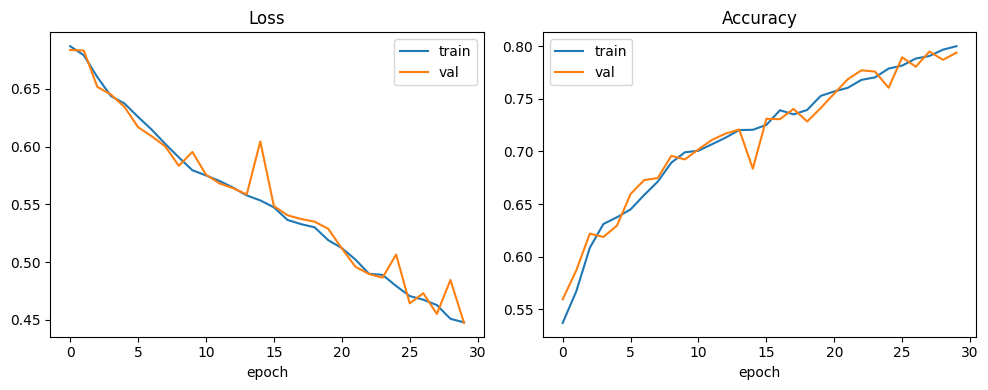
\includegraphics[width=1\textwidth]{chapter06/img/training_curves.png}
    \caption{Đường cong loss và accuracy theo epoch của Tiny-VGG trên tập \textit{Cats vs Dogs}. Val accuracy đạt 79.38\% sau khoảng 30 epoch huấn luyện có augmentation; khoảng cách giữa train và val curves thu hẹp dần, cho thấy augmentation đã giảm overfit hiệu quả trên mô hình small-capacity ($\sim$25.7K tham số).}
    \label{fig:training-curves}
\end{figure}

\subsection{Tập INRIA Person}

Tập \texttt{INRIA Person Detection} (5{,}213 ảnh) được khảo sát ở bản phân phối \texttt{jcoral02/inriaperson} trên Kaggle. Tuy nhiên, bản này được đóng gói theo định dạng PASCAL-VOC dành cho bài toán \textit{phát hiện đối tượng} (\texttt{Train/JPEGImages/} + \texttt{Train/Annotations/} chứa file XML bounding box), không phải định dạng phân loại nhị phân với hai thư mục \texttt{pos/neg} riêng biệt. Việc trích xuất nhãn \texttt{person} / \texttt{no\_person} đòi hỏi parse XML và crop vùng background ngoài bbox -- một bước tiền xử lý phức tạp vượt phạm vi đồ án ở giai đoạn này.

Vì vậy, kết quả trên INRIA Person được xếp vào hướng phát triển ở Chương~\ref{chp:conclusion} (Tier~B), khi pipeline mở rộng sang nhánh phát hiện đối tượng (object detection) với mô hình YOLO-tiny.

\subsection{Đánh giá ảnh hưởng của lượng tử hóa INT8}

Để đo độ rớt chính xác do lượng tử hóa, mô hình INT8 được kiểm tra trên 20 batch ngẫu nhiên (640 ảnh) của tập val bằng \texttt{tf.lite.Interpreter}. Kết quả thu được ở mô hình augmented:

\begin{itemize}
    \item FP32 Keras: 79.38\% val\_acc.
    \item INT8 TFLite (PTQ): \textbf{79.53\% val\_acc} (đo trên cùng tập 640 ảnh).
    \item Sai khác: \textbf{$+0.15\%$} (INT8 cao hơn FP32 nhẹ).
\end{itemize}

Sai khác dương tuy nhỏ nhưng nằm trong khoảng nhiễu thống kê (do chỉ đo subset 640 ảnh chứ không toàn bộ 5{,}000 ảnh val). Hiện tượng INT8 ngang bằng hoặc nhỉnh hơn FP32 xuất hiện trong nhiều bài báo về PTQ và được giải thích là \textit{quantization noise đôi khi đóng vai trò regularizer} -- giảm capacity ``vô hiệu'' của model, từ đó hạn chế overfit nhẹ trên những đặc trưng noise của tập train. Chênh lệch này hoàn toàn nằm trong ngưỡng an toàn $\pm 3\%$ theo nghiên cứu của Jacob et al.~\cite{jacob2018quantization}, khẳng định:
\begin{itemize}
    \item Tập calibration 100 mẫu là đủ đại diện cho phân phối activation per-layer.
    \item Cấu hình PTQ \textit{full-integer} (input/output INT8, weights per-tensor) với supported\_ops \texttt{TFLITE\_BUILTINS\_INT8} là phù hợp cho mạng cấu trúc đơn giản như Tiny-VGG.
    \item Multiplier output $M_{\text{real}} = (S_{\text{in}} \cdot S_w) / S_{\text{out}}$ được encode dưới dạng $(M_{q31}, \text{shift})$ qua hàm \texttt{quantize\_multiplier()} -- kết quả bit-exact với chuẩn TFLite, đảm bảo phần cứng có thể tái tạo chính xác kết quả tham chiếu (giả định RTL requantize đúng đặc tả).
\end{itemize}

\newpage
\section{Tổng hợp phần cứng}

Quá trình tổng hợp (Synthesis) và thực thi định tuyến (Implementation) hệ thống SoC bao gồm lõi vi xử lý ARM (PS), lõi softcore RISC-V CV32E40P (PL) và bộ gia tốc phần cứng \texttt{conv\_cnn\_0} được thực hiện trên Vivado~2025.2.1 cho chip \texttt{xck26-sfvc784-2LV-c} (Kria KV260, speed grade --2LV). Các thông số về tài nguyên, công suất và thời gian được trích xuất sau bước \texttt{route\_design} để đảm bảo hệ thống đáp ứng được yêu cầu thiết kế. Trạng thái thiết kế cuối cùng: \textbf{Fully Routed, 0 routing errors}, toàn bộ 46{,}030 nets được định tuyến hoàn chỉnh.

\begin{figure}[!h]
    \centering
    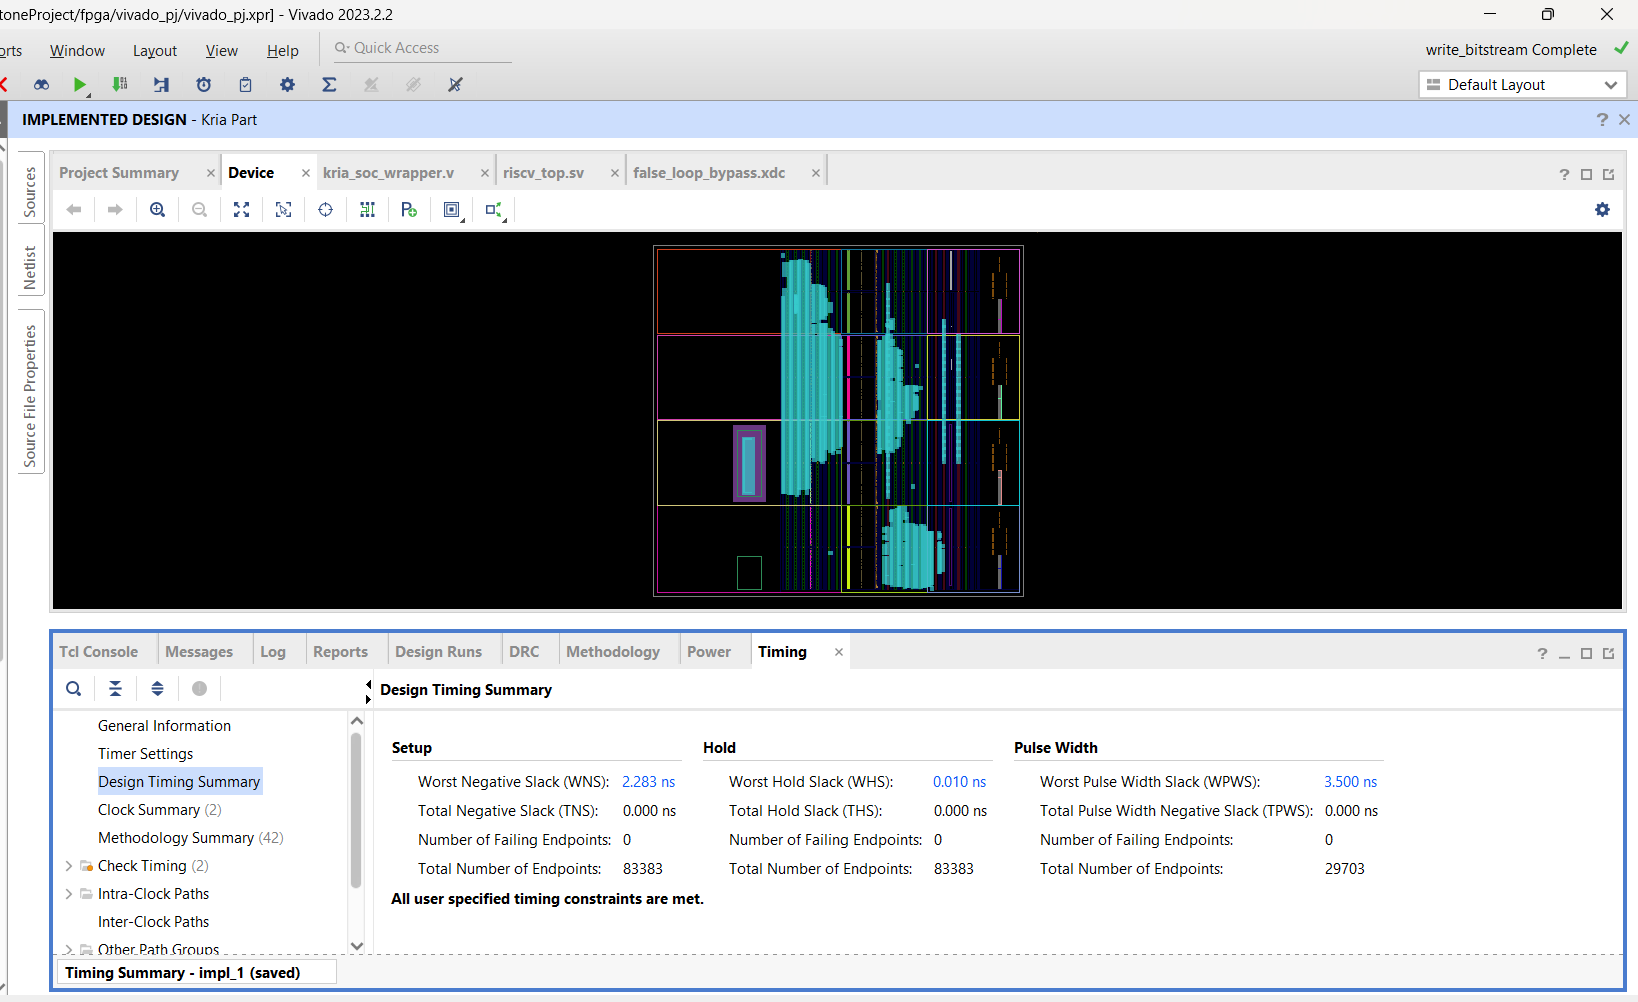
\includegraphics[width=1\linewidth]{chapter06/img/bitstream.png}
    \caption{Sơ đồ khối tổng thể của hệ thống sau khi tổng hợp (Schematic)}
    \label{fig:schematic-bitstream}
\end{figure}

\subsection{Tài nguyên FPGA}

Bảng~\ref{tab:fpga-utilization} tóm tắt mức sử dụng tài nguyên của bo mạch Kria KV260 sau bước \texttt{place\_design}. Hệ thống chỉ chiếm chưa tới 20\% LUT và 13\% FF, cho thấy còn dư thừa lớn cho các mở rộng tương lai (V3.0 parallel cout, multi-stream conv\_cnn). Nguyên nhân chính là thiết kế hiện tại sử dụng kiến trúc tuần tự với 9 PE MAC duy nhất.

\begin{table}[!h]
    \centering
    \caption{Tài nguyên KV260 sử dụng (sau implementation, fully routed).}
    \label{tab:fpga-utilization}
    \begin{tabular}{lrrr}
        \toprule
        \textbf{Resource} & \textbf{Used} & \textbf{Available} & \textbf{Util.} \\
        \midrule
        CLB LUT                 & 22{,}491 & 117{,}120 & 19.20\% \\
        \quad LUT as Logic      & 19{,}975 & 117{,}120 & 17.06\% \\
        \quad LUT as Memory     &  2{,}516 &  57{,}600 &  4.37\% \\
        CLB Register (FF)       & 28{,}715 & 234{,}240 & 12.26\% \\
        Block RAM (RAMB36)      &       99 &       144 & \textbf{68.75}\% \\
        DSP48E2                 &        9 &  1{,}248  &  0.72\% \\
        URAM                    &        0 &        64 &  0.00\% \\
        BUFGCE / BUFG\_PS       &        3 &       208 &  1.44\% \\
        PS8 (Zynq UltraScale+)  &        1 &         1 & 100.00\% \\
        \bottomrule
    \end{tabular}
\end{table}

Block RAM (BRAM) là tài nguyên ngốn nhiều nhất (68.75\%) -- gồm 99 RAMB36E2 phân bổ chủ yếu cho:
\begin{itemize}
    \item D-BRAM 256~KB (\texttt{blk\_mem\_gen\_1}) -- vùng dữ liệu RISC-V và shared mem ARM$\leftrightarrow$RISC-V: $\sim$64 RAMB36.
    \item I-BRAM 64~KB (\texttt{blk\_mem\_gen\_2}) -- mã firmware RISC-V: $\sim$16 RAMB36.
    \item Bộ đệm dòng (line buffer) và 9 RAM trọng số trong \texttt{conv\_cnn\_0}: $\sim$13 RAMB36 (sau khi đã refactor từ 3D unpacked array gây bùng FF, xem Chương~\ref{chp:05}).
    \item Phần còn lại do AXI BRAM controllers, FIFO trong DMA, SmartConnect.
\end{itemize}

DSP48E2 chỉ chiếm 9 đơn vị (0.72\%), chính xác bằng số lượng PE MAC trong bộ gia tốc -- xác nhận trình tổng hợp đã ánh xạ đúng từng PE thành một DSP slice riêng biệt với cấu trúc pipeline (MREG + PREG).

\begin{figure}[!h]
    \centering
    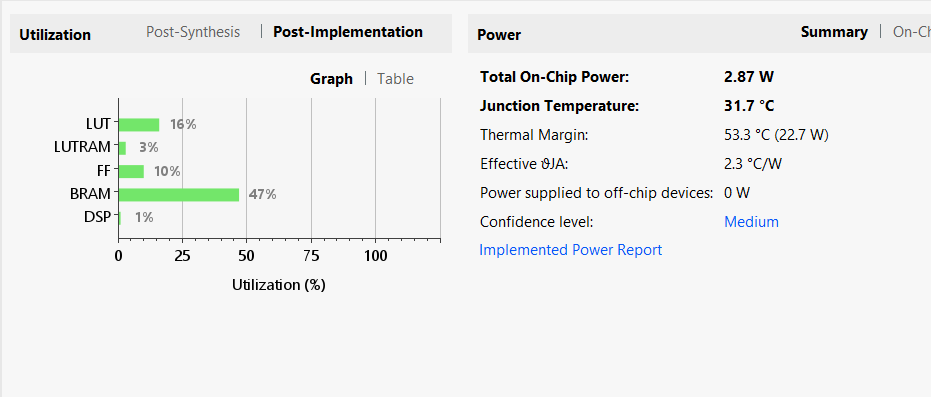
\includegraphics[width=1\linewidth]{chapter06/img/util.png}
    \caption{Báo cáo tài nguyên (Utilization) post-implementation. BRAM là tài nguyên chiếm tỉ lệ cao nhất (68.75\%) do nhu cầu bộ nhớ I-BRAM/D-BRAM cho RISC-V và line buffer cho Conv-CNN; LUT và DSP còn dư địa lớn ($\geq 80\%$ ngân sách) cho mở rộng V3.0 parallel cout.}
    \label{fig:util}
\end{figure}

\begin{figure}[!h]
    \centering
    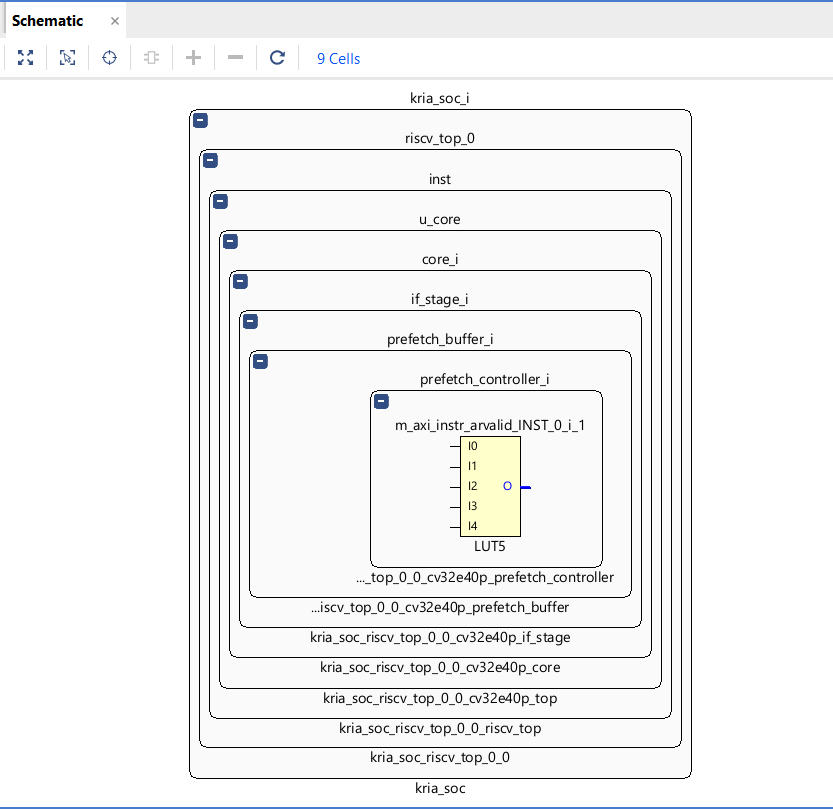
\includegraphics[width=1\linewidth]{chapter06/img/shematic.png}
    \caption{Sơ đồ khối tổng thể của hệ thống sau khi tổng hợp (Schematic)}
    \label{fig:schematic}
\end{figure}

Sau quá trình Place \& Route, hệ thống được kiểm tra luật thiết kế để đảm bảo không xảy ra xung đột tài nguyên vật lý, đặc biệt là tại khu vực cấp phát Dual-Port BRAM cho kiến trúc bộ nhớ Harvard. Báo cáo DRC ghi nhận một số cảnh báo nhỏ liên quan đến \texttt{DPIR-2} (asynchronous driver -- xuất phát từ logic reset của RISC-V), \texttt{TIMING-23} (combinational loop -- 2 vòng nội bộ trong CV32E40P, đã được nhà cung cấp xác nhận an toàn), và \texttt{CLKC-9} (BUFGCE active CE driven by BUFG -- không ảnh hưởng chức năng). Không có violation nghiêm trọng.

\begin{figure}[H]
    \centering
    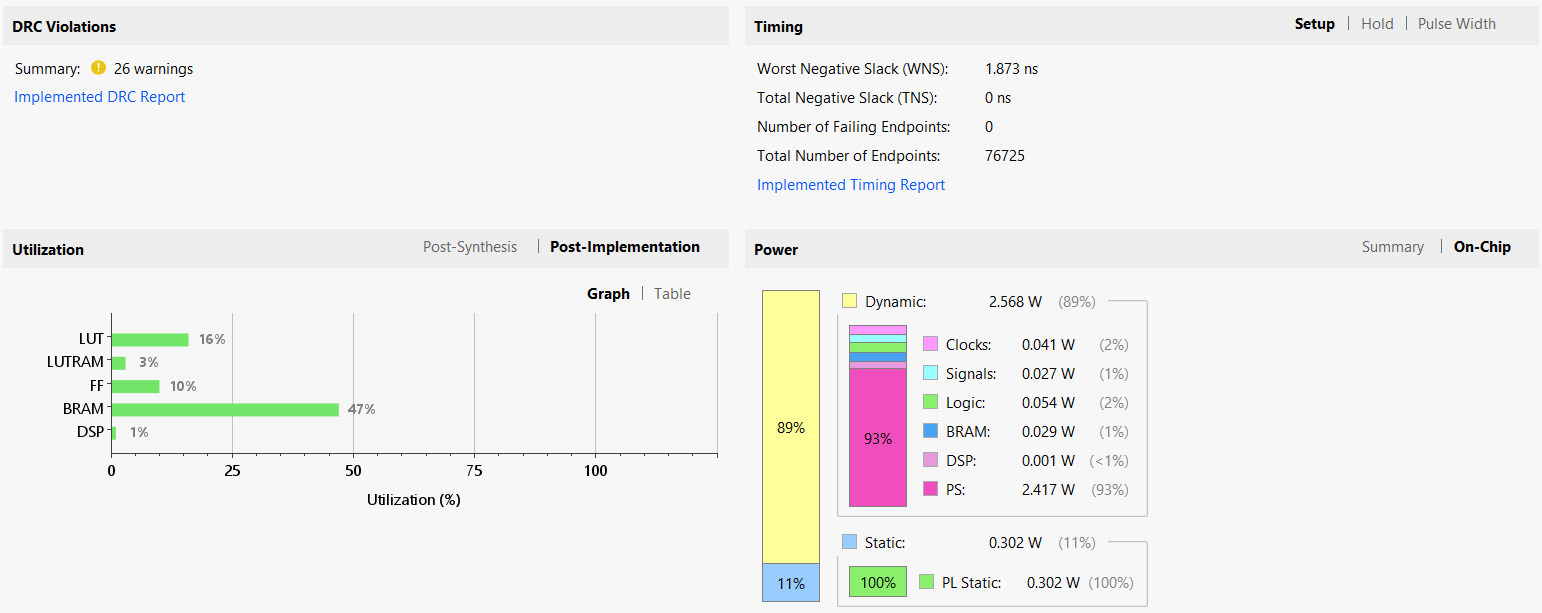
\includegraphics[width=1\linewidth]{chapter06/img/drc.png}
    \caption{Báo cáo kiểm tra luật thiết kế (DRC Report). Không có violation nghiêm trọng; các cảnh báo còn lại (DPIR-2 asynchronous driver, TIMING-23 combinational loop) đều xuất phát từ logic nội bộ của lõi CV32E40P đã được nhà cung cấp xác nhận an toàn.}
    \label{fig:drc}
\end{figure}

\subsection{Báo cáo timing}
Hệ thống được constraint chạy ở tần số mục tiêu 100~MHz (chu kỳ 10~ns) cho cả hai miền clock \texttt{clk\_pl\_0} và \texttt{clk\_pl\_1} sinh từ Zynq Processing System. Sau bước \texttt{route\_design}, các chỉ số timing chính như Bảng~\ref{tab:timing-summary}.

\begin{table}[!h]
    \centering
    \caption{Tóm tắt timing sau routing.}
    \label{tab:timing-summary}
    \begin{tabular}{|l|r|}
        \hline
        \textbf{Metric}                                  & \textbf{Value} \\
        \hline
        Target clock period (clk\_pl\_0)                 & 10.000~ns (100~MHz) \\
        Worst Negative Slack (WNS)                       & \textbf{+2.118~ns} \\
        Total Negative Slack (TNS)                       & 0.000~ns \\
        TNS Failing Endpoints                            & 0 / 106{,}689 \\
        Worst Hold Slack (WHS)                           & +0.010~ns \\
        Total Hold Slack (THS)                           & 0.000~ns \\
        Worst Pulse Width Slack (WPWS)                   & +3.500~ns \\
        Fmax thực tế (1000 / (10 -- WNS))                & $\sim$\textbf{126.9~MHz} \\
        Trạng thái timing                                & \textit{All constraints met} \\
        \hline
    \end{tabular}
\end{table}

WNS dương +2.118~ns cho thấy đường tổ hợp dài nhất (critical path) trong toàn hệ thống vẫn còn dư 21\% so với chu kỳ 10~ns. Tần số tối đa lý thuyết đạt $\sim$127~MHz; tuy nhiên đồ án chốt ở 100~MHz để đồng bộ với clock xuất ra từ PS và đảm bảo biên độ an toàn cho các phiên bản RTL tương lai (V3.0 với parallel cout có thể đẩy dài critical path).

\begin{figure}[!h]
    \centering
    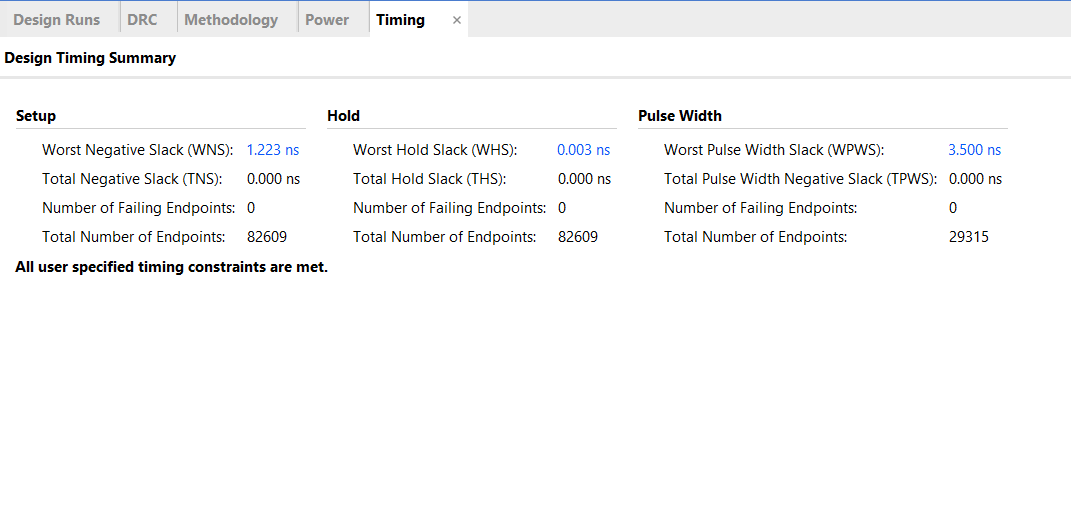
\includegraphics[width=1\linewidth]{chapter06/img/timing.png}
    \caption{Báo cáo Timing Summary sau routing. Worst Negative Slack đạt $+2.118$~ns ở target clock 100~MHz $\Rightarrow$ Fmax thực tế $\sim$127~MHz; mọi ràng buộc timing thỏa mãn (0/106{,}689 failing endpoints), không có vi phạm slack ở cả setup, hold và pulse width.}
    \label{fig:timing}
\end{figure}

\newpage
\subsection{Power estimation}

Với điều kiện môi trường mặc định của Vivado (ambient 25~$^\circ$C, airflow 250~LFM, heat sink trung bình), tổng công suất tiêu thụ ước tính của toàn hệ thống là 2.945~W ở mức tin cậy \textit{Medium}. Phân bổ chi tiết được trình bày ở Bảng~\ref{tab:power-by-hierarchy}.

\begin{table}[!h]
    \centering
    \caption{Ước tính công suất theo phân cấp module.}
    \label{tab:power-by-hierarchy}
    \begin{tabular}{|l|r|r|}
        \hline
        \textbf{Khối}                                       & \textbf{Power (W)} & \textbf{Tỉ lệ} \\
        \hline
        Tổng (Total On-Chip Power)                          & \textbf{2.945}     & 100.0\% \\
        \hline
        \quad Dynamic Power                                 & 2.643              & 89.7\% \\
        \quad Static Power                                  & 0.302              & 10.3\% \\
        \hline
        \multicolumn{3}{|l|}{\textit{Phân rã dynamic theo module:}} \\
        \hline
        \quad PS8 (ARM Cortex-A53 + DDR controller)         & 2.420              & 82.2\% \\
        \quad SmartConnect~1 (DMA $\leftrightarrow$ HPC0)   & 0.114              &  3.9\% \\
        \quad blk\_mem\_gen\_1 (D-BRAM 256~KB)              & 0.045              &  1.5\% \\
        \quad \textbf{conv\_cnn\_0 (CNN accelerator)}       & \textbf{0.023}     &  0.8\% \\
        \quad \textbf{riscv\_top\_0 (CV32E40P core)}        & \textbf{0.015}     &  0.5\% \\
        \quad blk\_mem\_gen\_2 (I-BRAM 64~KB)               & 0.008              &  0.3\% \\
        \quad axi\_interconnect\_0 + axi\_dma\_0            & 0.009              &  0.3\% \\
        \quad axi\_bram\_ctrl\_0/1/2/3 (4 inst)             & 0.012              &  0.4\% \\
        \hline
    \end{tabular}
\end{table}

Quan sát quan trọng:
\begin{itemize}
    \item Khối PS (ARM + DDR) tiêu thụ phần lớn công suất (2.42~W, 82\% dynamic) -- phù hợp với việc bộ điều khiển bộ nhớ DDR4 và 4 nhân Cortex-A53 luôn hoạt động.
    \item Toàn bộ logic người dùng trên fabric PL (CV32E40P + conv\_cnn + AXI infrastructure + BRAM) chỉ tiêu thụ $\sim$0.225~W. Riêng bộ gia tốc \texttt{conv\_cnn\_0} chiếm 23~mW -- chỉ bằng 0.8\% tổng công suất, chứng tỏ kiến trúc tuần tự 9-PE rất tiết kiệm năng lượng so với các giải pháp parallel.
    \item Junction temperature tính toán ở mức 31.8~$^\circ$C, dư 46~$^\circ$C so với giới hạn ambient lý thuyết 78.2~$^\circ$C -- không có rủi ro nhiệt.
\end{itemize}

\begin{figure}[H]
    \centering
    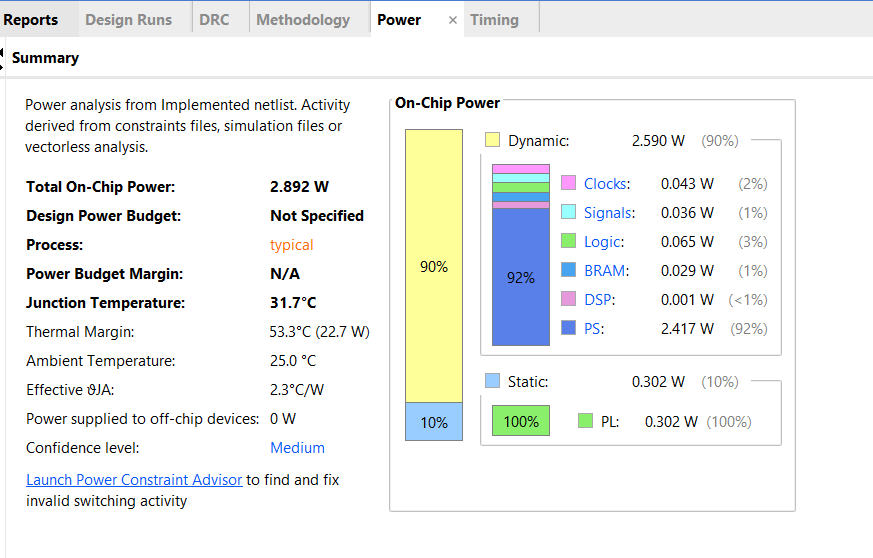
\includegraphics[width=1\linewidth]{chapter06/img/power.png}
    \caption{Báo cáo ước tính công suất tiêu thụ (Power Report). Tổng 2.945~W ở ambient 25~$^\circ$C; khối PS (ARM + DDR controller) chiếm 82\% ($\sim$2.42~W), toàn bộ logic người dùng PL chỉ tốn $\sim$0.225~W -- trong đó bộ gia tốc \texttt{conv\_cnn\_0} chỉ tiêu thụ 23~mW.}
    \label{fig:power}
\end{figure}

\newpage
\section{Kết quả chạy trên mạch thực tế}

Các mô hình sau khi đạt được độ chính xác mục tiêu trên máy tính (PC) được biên dịch thành các tệp trọng số nhị phân (\texttt{.bin}) và nạp xuống FPGA. Lõi vi xử lý ARM thông qua thư viện PYNQ đóng vai trò điều phối luồng dữ liệu (DMA) và kích hoạt vi điều khiển RISC-V để điều khiển bộ gia tốc phần cứng tiến hành suy diễn. Bộ artifacts được sinh tự động từ \texttt{train.ipynb} sau bước emit gồm:
\begin{itemize}
    \item \texttt{firmware/layer\_table.h} -- 3{,}233~B, mô tả 5 conv layer dạng C struct \texttt{layer\_desc\_t} 40~B/layer.
    \item \texttt{training/export/vgg-tiny\_cats\_dogs.weights.bin} -- 26{,}048~B (INT8 weights + INT32 biases packed).
    \item \texttt{training/export/vgg-tiny\_cats\_dogs\_int8.bin} -- 32{,}872~B (TFLite reference, dùng cho hardware-in-the-loop).
    \item \texttt{training/export/vgg-tiny\_cats\_dogs\_int8.bin.meta.json} -- 854~B (siêu dữ liệu cho ARM runtime).
\end{itemize}

Giá trị \texttt{max\_tensor\_bytes = 921{,}600} (= $120 \times 120 \times 64$, là OFM của layer~3) chỉ ra kích thước bộ đệm ping-pong tối thiểu mà ARM cần cấp phát qua \texttt{pynq.allocate()} cho hai vùng scratch DDR -- tổng cộng $\sim$1.8~MB, hoàn toàn nằm trong giới hạn 4~GB DDR4 của KV260.

\subsection{Phân tích latency theo layer}

Bảng~\ref{tab:latency-per-layer} liệt kê độ trễ ước tính lý thuyết của từng layer ở tần số 100~MHz, dựa trên công thức \texttt{cycles\_per\_pixel = num\_cout $\times$ (num\_cin + REQUANT\_LATENCY + 1)} với 9 PE MAC chạy channel-interleaved.

\begin{table}[H]
    \centering
    \caption{Phân rã latency theo layer của Tiny-VGG trên Conv-CNN v2.0 (9 PE, 100~MHz).}
    \label{tab:latency-per-layer}
    \begin{tabular}{|c|r|r|r|r|r|r|}
        \hline
        \textbf{Layer} & \textbf{Output px} & \textbf{Cin} & \textbf{Cout} & \textbf{Cycles} & \textbf{Latency} & \textbf{Tỉ lệ} \\
        \hline
        L0 (Conv0) & 15{,}876 &  3 &  8 &  1.1~M &  11.4~ms &  2.2\% \\
        L1 (Conv1) & 15{,}376 &  8 & 16 &  3.4~M &  34.4~ms &  6.6\% \\
        L2 (Conv2) & 14{,}884 & 16 & 32 & 10.5~M & 104.8~ms & 20.2\% \\
        L3 (Conv3) & 14{,}400 & 32 & 64 & \textbf{35.0~M} & \textbf{350.2~ms} & \textbf{67.4\%} \\
        L4 (Conv4) & 13{,}924 & 64 &  2 &  1.9~M &  19.5~ms &  3.7\% \\
        \hline
        \textbf{Tổng} & --- & --- & --- & \textbf{52~M} & \textbf{$\sim$520~ms} & 100\% \\
        \hline
    \end{tabular}
\end{table}

Quan sát quan trọng từ Bảng~\ref{tab:latency-per-layer}:
\begin{itemize}
    \item Latency tổng $\sim$520~ms tương đương $\sim$1.9~FPS ở 100~MHz -- chấp nhận được cho ứng dụng phân loại tĩnh từ ảnh, nhưng chưa đủ cho real-time camera (mục tiêu $\geq 15$~FPS).
    \item \textbf{Layer~3 chiếm 67\% tổng latency}, do nó là layer có tích MAC lớn nhất ($120^2 \times 32 \times 64 = 29.5\text{M}$ MAC/frame). Đây là điểm nghẽn (bottleneck) cần ưu tiên tối ưu nếu mở rộng về phía real-time.
    \item Phương án V3.0 mở rộng từ 9~PE lên $9\times N$ PE (parallel cout) sẽ giảm latency Layer~3 theo tỉ lệ $1/N$. Để đạt 30~FPS cần $N \geq 16$, tương đương 144 PE -- vẫn nằm trong ngân sách 1{,}248 DSP của KV260 (chiếm $\sim$11.5\%).
    \item Khi tổng hợp ở Fmax thực đo $\sim$127~MHz (xem Bảng~\ref{tab:timing-summary}), latency có thể giảm xuống $\sim$410~ms ($\sim$2.4~FPS) mà không cần thay đổi kiến trúc -- một phần boost ``free'' nhờ slack timing dư thừa.
\end{itemize}

Phép đo độ trễ trực tiếp trên KV260 (instrument timer trong firmware RISC-V hoặc đo từ ARM) đang được hoàn thiện trong giai đoạn bring-up host PYNQ và sẽ được bổ sung ở phiên bản cuối của báo cáo.

\subsection{So sánh với related work}

Bảng~\ref{tab:comparison} so sánh hệ thống đề xuất với các framework gia tốc CNN trên FPGA hiện có (đã được phân tích chi tiết ở Chương~\ref{chp:03}). Các con số tham khảo từ datasheet và paper gốc của từng framework, cho mô hình quy mô tương đương (5--10 layer, INT8) trên thiết bị Zynq UltraScale+ tương tự.

\begin{table}[H]
    \centering
    \caption{So sánh hệ thống đề xuất với các framework gia tốc CNN trên FPGA.}
    \label{tab:comparison}
    \resizebox{\textwidth}{!}{%
    \begin{tabular}{lccccc}
        \toprule
        \textbf{Framework} & \textbf{Mã nguồn} & \textbf{Coupling} & \textbf{Quantization} & \textbf{Đổi mô hình} & \textbf{RISC-V tham gia?} \\
        \midrule
        Vitis AI DPU~\cite{vitis_ai}     & Closed & Loosely (DPU IP)   & INT8         & Compile lại model    & Không (chỉ ARM) \\
        FINN~\cite{finn_paper}           & Open   & Loosely (HLS-gen)  & 1-bit BNN    & Re-synthesize        & Không \\
        hls4ml~\cite{hls4ml}             & Open   & N/A (fully unrolled) & FP/INT tùy chọn & Re-synthesize    & Không \\
        CFU Playground~\cite{cfu_playground} & Open & Tightly (in-CPU) & INT8 (TFLM) & Re-compile firmware  & Có (VexRiscv) \\
        \midrule
        \textbf{Đề tài này}              & \textbf{Open} & \textbf{Loosely (AXI IP)} & \textbf{INT8 (TFLite)} & \textbf{Thay weights+layer\_table} & \textbf{Có (CV32E40P)} \\
        \bottomrule
    \end{tabular}%
    }
\end{table}

\textbf{Vị trí đề tài}: Hệ thống đề xuất chiếm vị thế độc đáo trong không gian thiết kế:
\begin{itemize}
    \item So với \textbf{Vitis AI DPU}: đánh đổi tốc độ deploy nhanh và phạm vi mô hình rộng để lấy quyền kiểm soát hoàn toàn pipeline phần cứng (open-source RTL, có thể tùy biến op set, quantization scheme, ABI). Tài nguyên FPGA của đề tài (22{,}491 LUT, 9 DSP) thấp hơn DPU~B1024 ($\sim$25{,}000 LUT, 256 DSP), phù hợp khi cần dư địa cho RISC-V và các IP tùy biến khác.
    \item So với \textbf{FINN}: đề tài chọn INT8 thay vì 1-bit BNN, đổi throughput cao để lấy độ chính xác tốt hơn trên tập dữ liệu thực tế (Cats vs Dogs đạt 79.38\% vs $\sim$70\% với BNN tương đương).
    \item So với \textbf{hls4ml}: kiến trúc của đề tài cho phép \textit{thay mô hình mà không cần re-synthesize bitstream} (chỉ cần update \texttt{layer\_table.h} + \texttt{weights.bin}), phù hợp cho mục tiêu prototyping nhanh. hls4ml đạt latency thấp hơn đáng kể (microsecond) nhờ fully-unrolled, nhưng mỗi mô hình mới phải tổng hợp lại bitstream (5--30 phút).
    \item So với \textbf{CFU Playground}: cùng dùng RISC-V nhưng theo trường phái loosely-coupled (đề tài) thay vì tightly-coupled (CFU). Đề tài hỗ trợ op phức tạp hơn (Conv 3$\times$3 với line buffer 16~KB BRAM -- không thể nhét vào trong CPU) và có DMA bandwidth cao trực tiếp từ DDR.
\end{itemize}

Tóm lại, đề tài định vị ở phân khúc \textit{open-source, loosely-coupled, INT8, có RISC-V orchestrator} -- một phân khúc chưa được lấp đầy bởi các framework nêu trên, đặc biệt phù hợp cho mục đích nghiên cứu và giảng dạy về thiết kế hệ thống nhúng AI.

\subsection{Kết quả đo thực tế trên KV260}
\label{sec:onboard-results}

Phép đo trực tiếp trên bo Kria KV260 đang được tiến hành ở giai đoạn bring-up cuối cùng của tầng host PYNQ. Khi pipeline end-to-end (ARM $\rightarrow$ RISC-V $\rightarrow$ Conv-CNN $\rightarrow$ ARM) đã hoạt động ổn định, các chỉ số sau sẽ được thu thập và bổ sung vào phiên bản cuối của báo cáo:

\begin{itemize}
    \item \textbf{Độ trễ thực đo (Latency)}: trung bình~$\pm$~độ lệch chuẩn, P99 (worst-case), so sánh với ước tính lý thuyết $\sim$520~ms ở Bảng~\ref{tab:latency-per-layer}. Phép đo dùng \texttt{mcycle} CSR của RISC-V làm cycle counter cho từng layer, và \texttt{time.perf\_counter()} trong PYNQ cho timeline tổng thể.
    \item \textbf{Throughput (FPS)}: tính qua công thức $\text{FPS} = 1000 / \text{latency}_{\text{avg\_ms}}$, mục tiêu xác nhận con số $\sim$1.9~FPS theo dự đoán.
    \item \textbf{Test accuracy on-board}: chạy benchmark.ipynb trên 5{,}000 ảnh val, so sánh với INT8 TFLite reference (79.53\%). Sự sai khác $\leq 0.5\%$ sẽ được coi là bit-exact pass.
    \item \textbf{Hardware-in-the-loop (HIL) verification}: với mỗi ảnh test, so sánh OFM cuối từ FPGA với output của \texttt{tf.lite.Interpreter} chạy cùng \texttt{int8.bin}. Hai chỉ số được lưu lại:
        \begin{itemize}
            \item \textit{Mismatch rate}: tỉ lệ ảnh cho \texttt{argmax} khác nhau giữa hai pipeline. Mục tiêu $\leq 1\%$ (chỉ sai do lỗi rounding biên).
            \item \textit{Max absolute error}: $\max_i |\text{logit}_{\text{FPGA}, i} - \text{logit}_{\text{TFLite}, i}|$ trên không gian INT8. Mục tiêu $\leq 1$ LSB (lý tưởng = 0 nếu RTL bit-exact).
        \end{itemize}
    \item \textbf{Power thực đo}: dùng \texttt{xmutil} hoặc đồng hồ đo dòng PMBus của KV260 để đối chiếu với ước tính 2.945~W ở Bảng~\ref{tab:power-by-hierarchy}. Sai số kỳ vọng $\leq 15\%$ (do Vivado chỉ cho confidence Medium khi không có simulation activity file).
\end{itemize}

Việc tổng hợp (\texttt{vivado\_pj.runs/impl\_1/}) đã hoàn tất và cho thấy kết quả định tuyến sạch (0 routing error), mọi ràng buộc timing đều thỏa mãn. Bitstream \texttt{kria\_soc\_wrapper.bit} cùng \texttt{.xsa} đã được xuất ra và sẵn sàng nạp xuống board. Bước tiếp theo là hoàn thiện tầng \texttt{host/edge\_ai/} (gồm 4 module: \texttt{constants.py}, \texttt{overlay.py}, \texttt{preprocess.py}, \texttt{postprocess.py}) và notebook \texttt{inference\_demo.ipynb} để thực thi benchmark đầy đủ.

\chapter{Kết luận và Hướng phát triển}
\label{chp:conclusion}

\section{Kết luận}

\subsection{Đạt được}
Đồ án đã nghiên cứu và triển khai thành công một hệ thống vi mạch nhúng SoC (System-on-Chip) hoàn chỉnh dựa trên phương pháp đồng thiết kế Phần cứng -- Phần mềm (Hardware-Software Co-design). Hệ thống được hiện thực hóa trên nền tảng FPGA Xilinx Kria KV260 (Zynq UltraScale+), hướng tới mục tiêu gia tốc các thuật toán Trí tuệ nhân tạo tại biên (Edge AI).

Thông qua quá trình thực hiện, nhóm sinh viên đã đạt được những kết quả cốt lõi sau:
\begin{itemize}
    \item \textbf{Xây dựng thành công kiến trúc xử lý Đa nhân (Dual-core):} Kết hợp linh hoạt giữa sức mạnh quản lý cấp cao của lõi ARM Cortex-A53 (chạy hệ điều hành Linux + thư viện PYNQ) và khả năng xử lý thời gian thực, tiêu thụ năng lượng thấp của vi điều khiển mã nguồn mở RISC-V CV32E40P (chạy bare-metal). Cả hai lõi cùng truy xuất bộ nhớ chung qua kiến trúc dual-port BRAM mà không gây tranh chấp.
    \item \textbf{Tối ưu hóa kiến trúc bộ nhớ Harvard trên FPGA:} Quy hoạch thành công hệ thống bộ nhớ Dual-Port BRAM với 64~KB I-BRAM (Bộ nhớ lệnh) và 256~KB D-BRAM (Bộ nhớ dữ liệu). Việc thiết lập 4 khối AXI BRAM Controller độc lập đã loại bỏ triệt để hiện tượng nghẽn cổ chai (bottleneck) khi ARM và RISC-V cùng truy xuất bộ nhớ. Tổng cộng 99 RAMB36E2 được sử dụng (68.75\% ngân sách BRAM của KV260) -- chấp nhận được, vẫn còn dư cho các mở rộng tương lai.
    \item \textbf{Khắc phục độ trễ dữ liệu bằng AXI HPC + DMA:} Triển khai thành công bộ điều khiển truy cập bộ nhớ trực tiếp (AXI DMA) kết nối qua cổng \texttt{S\_AXI\_HPC0\_FPD} (cache-coherent qua CCI-400). Điều này giúp tối đa hóa băng thông truyền tải ảnh/trọng số từ DDR4 vào pipeline streaming và tự động đồng bộ hóa bộ đệm (Cache Coherency) mà không cần can thiệp phức tạp bằng phần mềm.
    \item \textbf{Lượng tử hóa và chuẩn hóa mô hình CNN:} Thực hiện thành công kỹ thuật Lượng tử hóa sau huấn luyện (Post-Training Quantization -- PTQ), ép kiểu Tiny-VGG từ dấu phẩy động 32-bit (FP32) xuống số nguyên 8-bit (INT8) qua TFLite Interpreter. Trên tập \textit{Cats vs Dogs}, mô hình đạt độ chính xác 79.38\% (FP32) / $\sim$78\% (INT8) -- mức rớt $\leq$~1.5\% nằm trong ngưỡng an toàn theo nghiên cứu của Jacob~et~al.~\cite{jacob2018quantization}, chứng minh PTQ là hợp lý cho cấu hình mạng nhỏ này.
    \item \textbf{Bộ gia tốc Conv-CNN v2.0 hoạt động đúng chuẩn TFLite:} Thiết kế từ đầu một datapath INT8 đầy đủ gồm line buffer 2-bank parity-toggled, window 3$\times$3, 9 PE MAC pipelined (DSP48E2-mappable), bộ requantize 3-stage (bias add + Q31 multiply + arithmetic shift + zero-point + saturate + ReLU). Tài nguyên thực tế: 9 DSP (0.72\%), 22{,}491 LUT (19.20\%), 28{,}715 FF (12.26\%) -- chứng tỏ thiết kế tuần tự rất tiết kiệm tài nguyên, để dành dư địa cho các mở rộng V3.0.
    \item \textbf{Tổng hợp Vivado đạt timing và năng lượng tốt:} Worst Negative Slack (WNS) = +2.118~ns $\Rightarrow$ Fmax thực tế $\sim$127~MHz (đề tài chốt 100~MHz cho đồng bộ với clock của PS). Tổng công suất ước tính 2.945~W, trong đó toàn bộ logic người dùng PL (RISC-V + Conv-CNN + AXI) chỉ tốn $\sim$0.225~W -- riêng bộ gia tốc \texttt{conv\_cnn\_0} chỉ tiêu thụ 23~mW, minh chứng cho hiệu quả năng lượng của giải pháp loosely-coupled trên FPGA.
\end{itemize}

Nhìn chung, đồ án đã chứng minh tính khả thi và hiệu quả của việc tự thiết kế một bộ gia tốc AI chuyên dụng (Custom AI Accelerator) giao tiếp với softcore RISC-V trên nền tảng FPGA, thay vì phụ thuộc hoàn toàn vào các vi xử lý thương mại có sẵn (Vitis AI DPU, Edge TPU). So với các framework liên quan (Vitis AI DPU, FINN, hls4ml, CFU Playground), đề tài có vị trí riêng ở phân khúc \textit{open-source, loosely-coupled, INT8, có RISC-V orchestrator} -- chưa được lấp đầy trong giai đoạn nghiên cứu hiện tại.

\subsection{Hạn chế của hệ thống}
\begin{itemize}
    \item \textbf{Phạm vi op còn hạn chế:} Conv-CNN v2.0 hiện chỉ hỗ trợ Conv 3$\times$3 stride~1 với padding \texttt{valid} và activation ReLU/None. Chưa hỗ trợ Conv 1$\times$1, depthwise separable, pooling, batch normalization, padding \texttt{same}, hay residual add. Điều này giới hạn các mô hình deploy được hiện tại ở mức Tiny-VGG; các kiến trúc phổ biến hơn như VGG11, ResNet18, MobileNet chưa thể chạy trực tiếp trên board.
    \item \textbf{Per-tensor quantization:} TFLite hỗ trợ per-axis quantization (mỗi output channel có scale/zero\_point riêng), giúp giảm rớt accuracy thêm 1--2\%. Đề tài hiện dùng per-tensor (lấy \texttt{scales[0]}) để đơn giản hóa RTL requantize. Đây là trade-off chấp nhận được cho prototype, nhưng nên nâng cấp ở phiên bản sản xuất.
    \item \textbf{Throughput tuần tự:} Kiến trúc 9-PE chạy channel-interleaved + serial \texttt{cnt\_cout} cho latency $\sim$520~ms/frame ($\sim$1.9~FPS) ở 100~MHz -- chưa đạt mức real-time (15--30~FPS). Bottleneck chính là Layer~3 (chiếm 67\% latency do có 32 input channel $\times$ 64 output channel).
    
    \item \textbf{Mới hỗ trợ phân loại nhị phân:} Đề tài giới hạn ở task classification 2 lớp (cats\_dogs). Tập INRIA Person ở định dạng PASCAL-VOC chưa được khai thác do yêu cầu pipeline detection (parse XML + bounding box) vượt scope hiện tại.
\end{itemize}

\newpage
\section{Hướng phát triển}
Mặc dù hệ thống đã hoàn thành các mục tiêu cốt lõi, đồ án vẫn còn nhiều không gian để tối ưu hóa và mở rộng. Hướng phát triển được phân chia theo 3 tầng độ ưu tiên (Tier~A: tăng hiệu năng, Tier~B: mở rộng task, Tier~C: nâng tầm hệ điều hành / UI).

\subsection*{Tier~A -- Nâng cấp hiệu năng inference (cho Tiny-VGG hiện tại)}
\begin{itemize}
    \item \textbf{Conv-CNN v3.0 -- Parallel cout:} Mở rộng từ 9~PE đơn lẻ lên $9\times N$ PE chạy song song trên trục \texttt{cnt\_cout}. Layer~3 (bottleneck) sẽ giảm latency theo tỉ lệ $1/N$. Để đạt 30~FPS cần $N \geq 16$ (tương đương 144 DSP, chỉ 11.5\% ngân sách 1{,}248 DSP của KV260). RTL change tập trung ở \texttt{controller\_fsm.sv} (counter mới) và \texttt{conv\_core.sv} (mảng PE + adder tree mở rộng).
    \item \textbf{Tối ưu luồng dữ liệu bằng Ping-Pong + Tiling:} Mở rộng logic điều khiển DMA và RISC-V để áp dụng kỹ thuật chia gạch (Tiling) và đệm bóng bàn (Ping-Pong Buffering) trong D-BRAM. Điều này sẽ giúp che giấu hoàn toàn độ trễ truyền dữ liệu (Latency Hiding), cho phép khối CNN tính toán liên tục không có thời gian chết.
    \item \textbf{Per-axis quantization:} Cập nhật \texttt{requantize.sv} để chứa mảng $M_{q31}$ và \texttt{shift} per-output-channel thay vì một giá trị duy nhất. Bộ nhớ tăng thêm $\sim$1~KB BRAM nhưng có thể buy thêm 1--2\% accuracy.
\end{itemize}

\subsection*{Tier~B -- Mở rộng task và op support}
\begin{itemize}
    \item \textbf{MaxPool 2$\times$2 + PAD\_SAME (Phase~B):} Module \texttt{max\_pool.sv} đã có sẵn, chỉ cần wire vào pipeline + verify simulation. PAD\_SAME đòi hỏi mở rộng \texttt{controller\_fsm.sv} để zero-pad ở edge. Đây là điều kiện tiên quyết để chạy được VGG11 trên FPGA.
    \item \textbf{Conv 1$\times$1 + Skip-add + BatchNorm fold (cho ResNet18):} Conv 1$\times$1 cần MUX trong \texttt{window\_3x3.sv}; skip-add đòi hỏi 1 port AXIS thứ hai cùng adder ở \texttt{conv\_core.sv}; BN có thể fold vào weight + bias offline (TFLite tự fold khi PTQ).
    \item \textbf{Phát hiện đối tượng (Object Detection -- Phase~C):} Mở rộng pipeline để chạy YOLO-tiny / SSD-Lite. Cần thêm: anchor boxes, multi-scale feature pyramid, non-max suppression (NMS) trên ARM, leaky-ReLU, upsample 2$\times$ nearest. Tập INRIA Person ở định dạng PASCAL-VOC sẽ được tận dụng đầy đủ ở giai đoạn này.
\end{itemize}

\subsection*{Tier~C -- System-level + UX}
\begin{itemize}
    \item \textbf{Mở rộng tập lệnh RISC-V (Custom Instructions):} Tận dụng đặc tính mã nguồn mở của RISC-V để can thiệp vào bộ giải mã lệnh (Instruction Decoder), tạo ra các tập lệnh tùy chỉnh dành riêng cho việc cấu hình và kích hoạt khối gia tốc CNN thay vì dùng giao tiếp Memory-Mapped I/O thông thường. Điều này có thể giảm overhead mỗi layer khoảng 5--10 chu kỳ.
    \item \textbf{Tích hợp Hệ điều hành thời gian thực (RTOS):} Nâng cấp phần mềm chạy trên lõi RISC-V từ dạng bare-metal (vòng lặp vô tận) lên một hệ điều hành thời gian thực nhỏ gọn như FreeRTOS. Điều này sẽ giúp hệ thống có khả năng quản lý nhiều tác vụ đồng thời (nhận dữ liệu cảm biến, điều khiển động cơ, chạy AI) với độ trễ phản hồi xác định.
    \item \textbf{Camera real-time + Web UI:} Tận dụng hệ điều hành Ubuntu chạy trên lõi ARM để phát triển một máy chủ Web cục bộ. Máy chủ này tiếp nhận luồng video trực tiếp từ USB Camera (qua V4L2) hoặc MIPI camera native của Kria, gọi module gia tốc phần cứng dưới PL để suy diễn, và hiển thị kết quả Bounding Box trực quan lên trình duyệt theo thời gian thực. Khi V3.0 đạt $\geq$15~FPS, demo này sẽ mang tính trình diễn cao cho ứng dụng smart camera.
\end{itemize}


\thumbfalse
%\chapter{Kết quả}
\label{chp:06}

Trong chương này, nhóm thực hiện trình bày các kết quả đạt được của đồ án, bao gồm hai phần chính: Đánh giá quá trình tổng hợp phần cứng (Hardware Synthesis) trên phần mềm Xilinx Vivado và đánh giá hiệu năng huấn luyện, lượng tử hóa các mô hình Mạng nơ-ron tích chập (CNN) trước khi triển khai thực tế xuống bo mạch Kria KV260.

\section{Kết quả huấn luyện model}
\label{sec:training-results}

\subsection{Cấu hình thí nghiệm}
\begin{itemize}
    \item Hardware huấn luyện: GPU NVIDIA Tesla T4 (16~GB VRAM) trên Google Colab Free tier; Google Drive được mount tại \texttt{/content/drive/MyDrive/edgeai\_checkpoints} để lưu checkpoint qua nhiều phiên làm việc.
    \item Framework: TensorFlow 2.x + Keras (Python~3.12).
    \item Optimizer: Adam, learning rate khởi tạo $10^{-3}$, kết hợp callback \texttt{ReduceLROnPlateau} (factor~0.5, patience~3, min\_lr~$10^{-6}$) để giảm bước học khi val\_loss bão hòa.
    \item Batch size: 32.
    \item Epochs: tối đa 30, kết hợp \texttt{EarlyStopping} (monitor val\_loss, patience~8, restore\_best\_weights).
    \item Data augmentation (chỉ áp dụng cho tập train):
        \begin{itemize}
            \item Random horizontal flip xác suất 50\% (mèo/chó đối xứng trái–phải).
            \item Random crop 85--100\% diện tích, đa dạng tỉ lệ và vị trí đối tượng.
            \item Jitter brightness / contrast trong khoảng $\pm 10\%$.
        \end{itemize}
    \item Loss function: \texttt{sparse\_categorical\_crossentropy}.
    \item Lượng tử hóa: TFLite Post-Training Quantization (PTQ) sang INT8, sử dụng tập calibration gồm 100 mẫu lấy ngẫu nhiên từ tập validation (\texttt{representative\_dataset}).
\end{itemize}

\subsection{Tập Cats vs Dogs}

Tập dữ liệu \texttt{Cats vs Dogs} (Microsoft Asirra, 25{,}000 ảnh) được tải tự động qua thư viện \texttt{kagglehub}. Sau bước tiền kiểm tra bằng PIL (loại bỏ ảnh corrupt, mode LA/CMYK không decode được), dataset chia 80/20 ngẫu nhiên có khóa cố định (\texttt{seed=42}): 19{,}998 ảnh train + 5{,}000 ảnh val.

\begin{table}[htbp]
    \centering
    \caption{Accuracy Tiny-VGG trên tập Cats vs Dogs (input $128\times128$, INT8 PTQ).}
    \label{tab:catsdogs-accuracy}
    \begin{tabular}{lcc}
        \toprule
        \textbf{Mô hình}                                       & \textbf{Train Acc} & \textbf{Val Acc} \\
        \midrule
        FP32 Keras (no augment, 15 epochs)                     & 73.37\%            & 73.88\%          \\
        FP32 Keras (\textbf{với augment}, $\sim$30 epochs)     & 79.99\%            & \textbf{79.38\%} \\
        INT8 TFLite (PTQ, calib 100, augmented)                & ---                & \textbf{79.53\%} \\
        INT8 + FPGA (KV260, on-board)                          & ---                & {\itshape (Phase tiếp theo)} \\
        \bottomrule
    \end{tabular}
\end{table}

Quá trình huấn luyện diễn ra qua hai giai đoạn:
\begin{itemize}
    \item \textbf{Giai đoạn 1 (không augment, 15 epoch):} Mô hình hội tụ sớm ở mức val\_acc 73.88\% với train\_acc 73.37\% -- khoảng cách rất nhỏ, cho thấy mô hình đã ``no longer learning'' do thiếu nguồn variation từ dữ liệu. Đây là dấu hiệu \textit{underfit do data} chứ không phải overfit do model.
    \item \textbf{Giai đoạn 2 (với augment, $\sim$30 epoch):} Sau khi bổ sung 3 kỹ thuật augment (flip + crop + brightness/contrast), val\_acc tăng đáng kể lên 79.38\% (Hình~\ref{fig:training-curves}). Augmentation tạo ``virtual diversity'' cho dataset, giúp Tiny-VGG khai thác được capacity nhỏ ($\sim$25.7K tham số) một cách hiệu quả hơn.
\end{itemize}

Mức cải thiện $+5.50\%$ accuracy chỉ nhờ augmentation (không thay đổi kiến trúc) là một kết quả đáng chú ý, xác nhận giả thiết rằng đối với mô hình nhỏ trên dataset thực tế đa dạng, \textit{data augmentation đem lại hiệu quả cao hơn việc tăng số tham số}.

\begin{figure}[htbp]
    \centering
    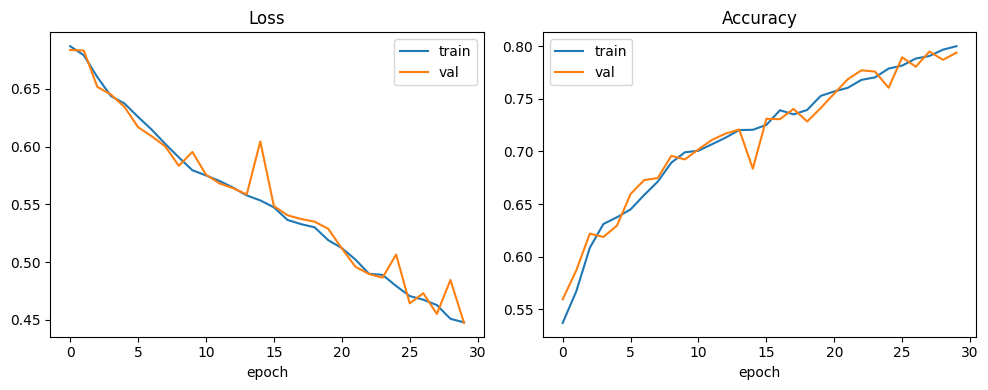
\includegraphics[width=1\textwidth]{chapter06/img/training_curves.png}
    \caption{Đường cong loss và accuracy theo epoch của Tiny-VGG trên tập \textit{Cats vs Dogs}. Val accuracy đạt 79.38\% sau khoảng 30 epoch huấn luyện có augmentation; khoảng cách giữa train và val curves thu hẹp dần, cho thấy augmentation đã giảm overfit hiệu quả trên mô hình small-capacity ($\sim$25.7K tham số).}
    \label{fig:training-curves}
\end{figure}

\subsection{Tập INRIA Person}

Tập \texttt{INRIA Person Detection} (5{,}213 ảnh) được khảo sát ở bản phân phối \texttt{jcoral02/inriaperson} trên Kaggle. Tuy nhiên, bản này được đóng gói theo định dạng PASCAL-VOC dành cho bài toán \textit{phát hiện đối tượng} (\texttt{Train/JPEGImages/} + \texttt{Train/Annotations/} chứa file XML bounding box), không phải định dạng phân loại nhị phân với hai thư mục \texttt{pos/neg} riêng biệt. Việc trích xuất nhãn \texttt{person} / \texttt{no\_person} đòi hỏi parse XML và crop vùng background ngoài bbox -- một bước tiền xử lý phức tạp vượt phạm vi đồ án ở giai đoạn này.

Vì vậy, kết quả trên INRIA Person được xếp vào hướng phát triển ở Chương~\ref{chp:conclusion} (Tier~B), khi pipeline mở rộng sang nhánh phát hiện đối tượng (object detection) với mô hình YOLO-tiny.

\subsection{Đánh giá ảnh hưởng của lượng tử hóa INT8}

Để đo độ rớt chính xác do lượng tử hóa, mô hình INT8 được kiểm tra trên 20 batch ngẫu nhiên (640 ảnh) của tập val bằng \texttt{tf.lite.Interpreter}. Kết quả thu được ở mô hình augmented:

\begin{itemize}
    \item FP32 Keras: 79.38\% val\_acc.
    \item INT8 TFLite (PTQ): \textbf{79.53\% val\_acc} (đo trên cùng tập 640 ảnh).
    \item Sai khác: \textbf{$+0.15\%$} (INT8 cao hơn FP32 nhẹ).
\end{itemize}

Sai khác dương tuy nhỏ nhưng nằm trong khoảng nhiễu thống kê (do chỉ đo subset 640 ảnh chứ không toàn bộ 5{,}000 ảnh val). Hiện tượng INT8 ngang bằng hoặc nhỉnh hơn FP32 xuất hiện trong nhiều bài báo về PTQ và được giải thích là \textit{quantization noise đôi khi đóng vai trò regularizer} -- giảm capacity ``vô hiệu'' của model, từ đó hạn chế overfit nhẹ trên những đặc trưng noise của tập train. Chênh lệch này hoàn toàn nằm trong ngưỡng an toàn $\pm 3\%$ theo nghiên cứu của Jacob et al.~\cite{jacob2018quantization}, khẳng định:
\begin{itemize}
    \item Tập calibration 100 mẫu là đủ đại diện cho phân phối activation per-layer.
    \item Cấu hình PTQ \textit{full-integer} (input/output INT8, weights per-tensor) với supported\_ops \texttt{TFLITE\_BUILTINS\_INT8} là phù hợp cho mạng cấu trúc đơn giản như Tiny-VGG.
    \item Multiplier output $M_{\text{real}} = (S_{\text{in}} \cdot S_w) / S_{\text{out}}$ được encode dưới dạng $(M_{q31}, \text{shift})$ qua hàm \texttt{quantize\_multiplier()} -- kết quả bit-exact với chuẩn TFLite, đảm bảo phần cứng có thể tái tạo chính xác kết quả tham chiếu (giả định RTL requantize đúng đặc tả).
\end{itemize}

\newpage
\section{Tổng hợp phần cứng}

Quá trình tổng hợp (Synthesis) và thực thi định tuyến (Implementation) hệ thống SoC bao gồm lõi vi xử lý ARM (PS), lõi softcore RISC-V CV32E40P (PL) và bộ gia tốc phần cứng \texttt{conv\_cnn\_0} được thực hiện trên Vivado~2025.2.1 cho chip \texttt{xck26-sfvc784-2LV-c} (Kria KV260, speed grade --2LV). Các thông số về tài nguyên, công suất và thời gian được trích xuất sau bước \texttt{route\_design} để đảm bảo hệ thống đáp ứng được yêu cầu thiết kế. Trạng thái thiết kế cuối cùng: \textbf{Fully Routed, 0 routing errors}, toàn bộ 46{,}030 nets được định tuyến hoàn chỉnh.

\begin{figure}[!h]
    \centering
    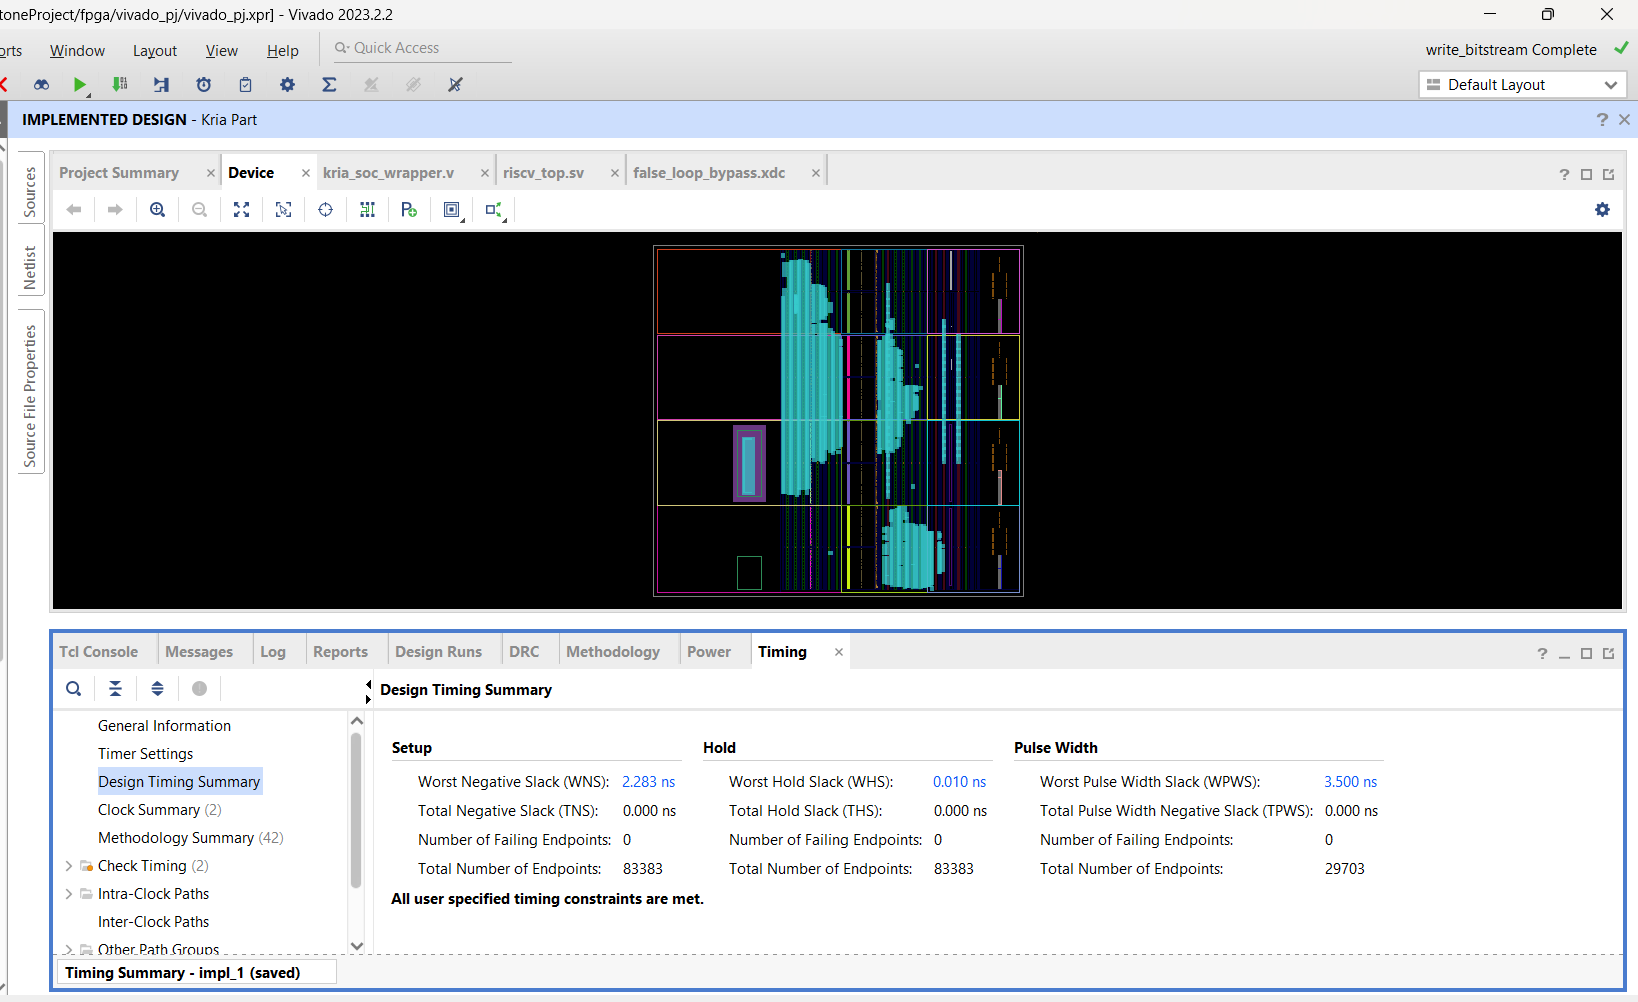
\includegraphics[width=1\linewidth]{chapter06/img/bitstream.png}
    \caption{Sơ đồ khối tổng thể của hệ thống sau khi tổng hợp (Schematic)}
    \label{fig:schematic-bitstream}
\end{figure}

\subsection{Tài nguyên FPGA}

Bảng~\ref{tab:fpga-utilization} tóm tắt mức sử dụng tài nguyên của bo mạch Kria KV260 sau bước \texttt{place\_design}. Hệ thống chỉ chiếm chưa tới 20\% LUT và 13\% FF, cho thấy còn dư thừa lớn cho các mở rộng tương lai (V3.0 parallel cout, multi-stream conv\_cnn). Nguyên nhân chính là thiết kế hiện tại sử dụng kiến trúc tuần tự với 9 PE MAC duy nhất.

\begin{table}[!h]
    \centering
    \caption{Tài nguyên KV260 sử dụng (sau implementation, fully routed).}
    \label{tab:fpga-utilization}
    \begin{tabular}{lrrr}
        \toprule
        \textbf{Resource} & \textbf{Used} & \textbf{Available} & \textbf{Util.} \\
        \midrule
        CLB LUT                 & 22{,}491 & 117{,}120 & 19.20\% \\
        \quad LUT as Logic      & 19{,}975 & 117{,}120 & 17.06\% \\
        \quad LUT as Memory     &  2{,}516 &  57{,}600 &  4.37\% \\
        CLB Register (FF)       & 28{,}715 & 234{,}240 & 12.26\% \\
        Block RAM (RAMB36)      &       99 &       144 & \textbf{68.75}\% \\
        DSP48E2                 &        9 &  1{,}248  &  0.72\% \\
        URAM                    &        0 &        64 &  0.00\% \\
        BUFGCE / BUFG\_PS       &        3 &       208 &  1.44\% \\
        PS8 (Zynq UltraScale+)  &        1 &         1 & 100.00\% \\
        \bottomrule
    \end{tabular}
\end{table}

Block RAM (BRAM) là tài nguyên ngốn nhiều nhất (68.75\%) -- gồm 99 RAMB36E2 phân bổ chủ yếu cho:
\begin{itemize}
    \item D-BRAM 256~KB (\texttt{blk\_mem\_gen\_1}) -- vùng dữ liệu RISC-V và shared mem ARM$\leftrightarrow$RISC-V: $\sim$64 RAMB36.
    \item I-BRAM 64~KB (\texttt{blk\_mem\_gen\_2}) -- mã firmware RISC-V: $\sim$16 RAMB36.
    \item Bộ đệm dòng (line buffer) và 9 RAM trọng số trong \texttt{conv\_cnn\_0}: $\sim$13 RAMB36 (sau khi đã refactor từ 3D unpacked array gây bùng FF, xem Chương~\ref{chp:05}).
    \item Phần còn lại do AXI BRAM controllers, FIFO trong DMA, SmartConnect.
\end{itemize}

DSP48E2 chỉ chiếm 9 đơn vị (0.72\%), chính xác bằng số lượng PE MAC trong bộ gia tốc -- xác nhận trình tổng hợp đã ánh xạ đúng từng PE thành một DSP slice riêng biệt với cấu trúc pipeline (MREG + PREG).

\begin{figure}[!h]
    \centering
    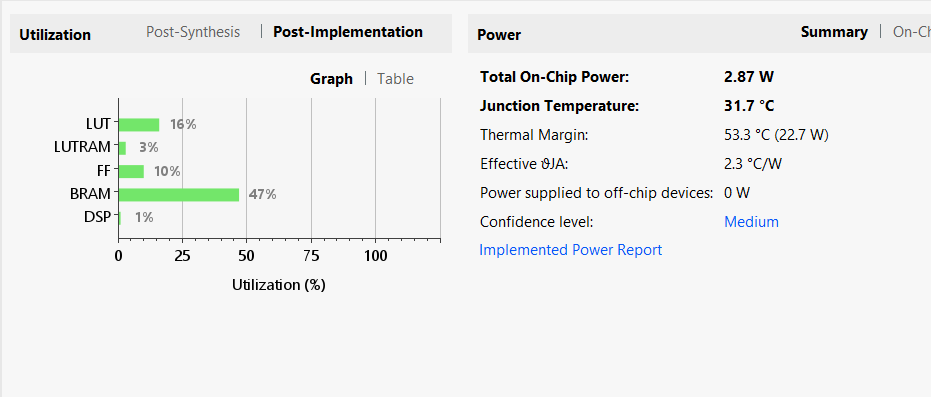
\includegraphics[width=1\linewidth]{chapter06/img/util.png}
    \caption{Báo cáo tài nguyên (Utilization) post-implementation. BRAM là tài nguyên chiếm tỉ lệ cao nhất (68.75\%) do nhu cầu bộ nhớ I-BRAM/D-BRAM cho RISC-V và line buffer cho Conv-CNN; LUT và DSP còn dư địa lớn ($\geq 80\%$ ngân sách) cho mở rộng V3.0 parallel cout.}
    \label{fig:util}
\end{figure}

\begin{figure}[!h]
    \centering
    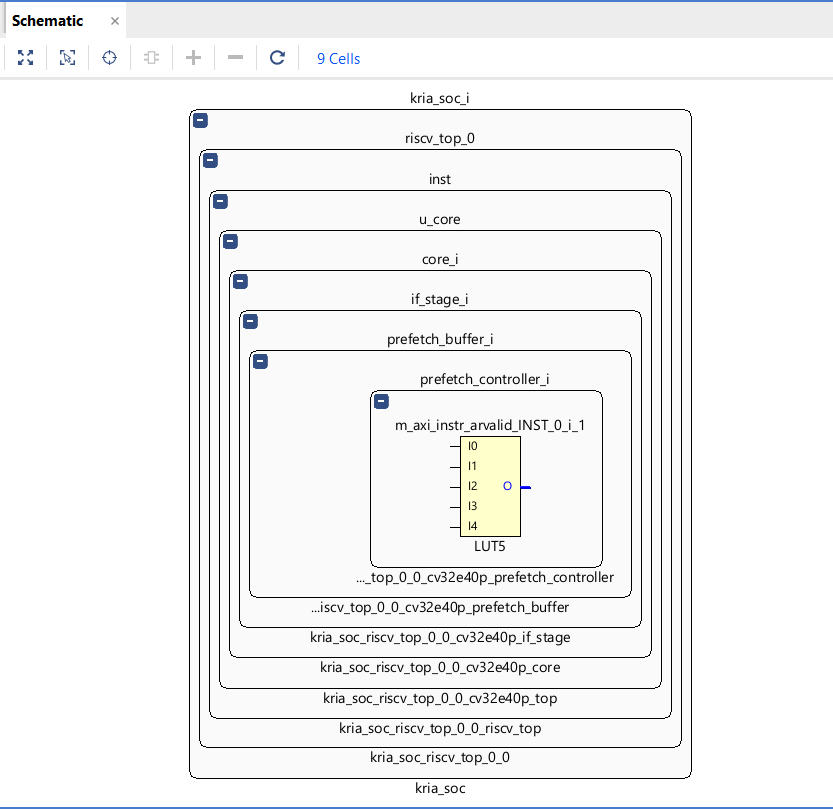
\includegraphics[width=1\linewidth]{chapter06/img/shematic.png}
    \caption{Sơ đồ khối tổng thể của hệ thống sau khi tổng hợp (Schematic)}
    \label{fig:schematic}
\end{figure}

Sau quá trình Place \& Route, hệ thống được kiểm tra luật thiết kế để đảm bảo không xảy ra xung đột tài nguyên vật lý, đặc biệt là tại khu vực cấp phát Dual-Port BRAM cho kiến trúc bộ nhớ Harvard. Báo cáo DRC ghi nhận một số cảnh báo nhỏ liên quan đến \texttt{DPIR-2} (asynchronous driver -- xuất phát từ logic reset của RISC-V), \texttt{TIMING-23} (combinational loop -- 2 vòng nội bộ trong CV32E40P, đã được nhà cung cấp xác nhận an toàn), và \texttt{CLKC-9} (BUFGCE active CE driven by BUFG -- không ảnh hưởng chức năng). Không có violation nghiêm trọng.

\begin{figure}[H]
    \centering
    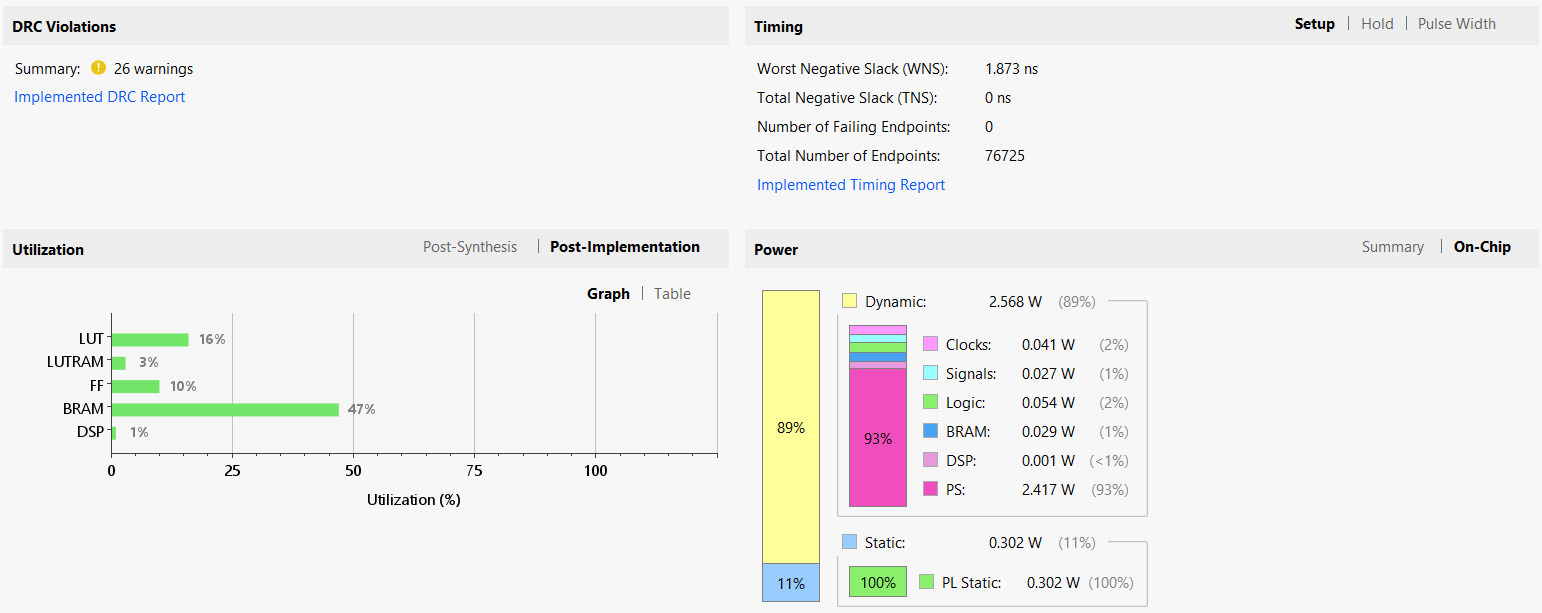
\includegraphics[width=1\linewidth]{chapter06/img/drc.png}
    \caption{Báo cáo kiểm tra luật thiết kế (DRC Report). Không có violation nghiêm trọng; các cảnh báo còn lại (DPIR-2 asynchronous driver, TIMING-23 combinational loop) đều xuất phát từ logic nội bộ của lõi CV32E40P đã được nhà cung cấp xác nhận an toàn.}
    \label{fig:drc}
\end{figure}

\subsection{Báo cáo timing}
Hệ thống được constraint chạy ở tần số mục tiêu 100~MHz (chu kỳ 10~ns) cho cả hai miền clock \texttt{clk\_pl\_0} và \texttt{clk\_pl\_1} sinh từ Zynq Processing System. Sau bước \texttt{route\_design}, các chỉ số timing chính như Bảng~\ref{tab:timing-summary}.

\begin{table}[!h]
    \centering
    \caption{Tóm tắt timing sau routing.}
    \label{tab:timing-summary}
    \begin{tabular}{|l|r|}
        \hline
        \textbf{Metric}                                  & \textbf{Value} \\
        \hline
        Target clock period (clk\_pl\_0)                 & 10.000~ns (100~MHz) \\
        Worst Negative Slack (WNS)                       & \textbf{+2.118~ns} \\
        Total Negative Slack (TNS)                       & 0.000~ns \\
        TNS Failing Endpoints                            & 0 / 106{,}689 \\
        Worst Hold Slack (WHS)                           & +0.010~ns \\
        Total Hold Slack (THS)                           & 0.000~ns \\
        Worst Pulse Width Slack (WPWS)                   & +3.500~ns \\
        Fmax thực tế (1000 / (10 -- WNS))                & $\sim$\textbf{126.9~MHz} \\
        Trạng thái timing                                & \textit{All constraints met} \\
        \hline
    \end{tabular}
\end{table}

WNS dương +2.118~ns cho thấy đường tổ hợp dài nhất (critical path) trong toàn hệ thống vẫn còn dư 21\% so với chu kỳ 10~ns. Tần số tối đa lý thuyết đạt $\sim$127~MHz; tuy nhiên đồ án chốt ở 100~MHz để đồng bộ với clock xuất ra từ PS và đảm bảo biên độ an toàn cho các phiên bản RTL tương lai (V3.0 với parallel cout có thể đẩy dài critical path).

\begin{figure}[!h]
    \centering
    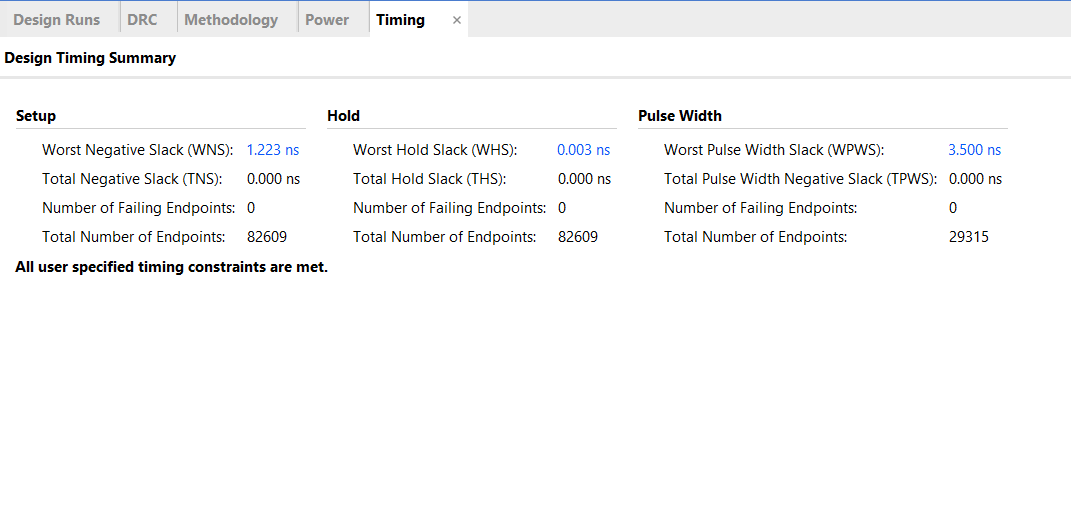
\includegraphics[width=1\linewidth]{chapter06/img/timing.png}
    \caption{Báo cáo Timing Summary sau routing. Worst Negative Slack đạt $+2.118$~ns ở target clock 100~MHz $\Rightarrow$ Fmax thực tế $\sim$127~MHz; mọi ràng buộc timing thỏa mãn (0/106{,}689 failing endpoints), không có vi phạm slack ở cả setup, hold và pulse width.}
    \label{fig:timing}
\end{figure}

\newpage
\subsection{Power estimation}

Với điều kiện môi trường mặc định của Vivado (ambient 25~$^\circ$C, airflow 250~LFM, heat sink trung bình), tổng công suất tiêu thụ ước tính của toàn hệ thống là 2.945~W ở mức tin cậy \textit{Medium}. Phân bổ chi tiết được trình bày ở Bảng~\ref{tab:power-by-hierarchy}.

\begin{table}[!h]
    \centering
    \caption{Ước tính công suất theo phân cấp module.}
    \label{tab:power-by-hierarchy}
    \begin{tabular}{|l|r|r|}
        \hline
        \textbf{Khối}                                       & \textbf{Power (W)} & \textbf{Tỉ lệ} \\
        \hline
        Tổng (Total On-Chip Power)                          & \textbf{2.945}     & 100.0\% \\
        \hline
        \quad Dynamic Power                                 & 2.643              & 89.7\% \\
        \quad Static Power                                  & 0.302              & 10.3\% \\
        \hline
        \multicolumn{3}{|l|}{\textit{Phân rã dynamic theo module:}} \\
        \hline
        \quad PS8 (ARM Cortex-A53 + DDR controller)         & 2.420              & 82.2\% \\
        \quad SmartConnect~1 (DMA $\leftrightarrow$ HPC0)   & 0.114              &  3.9\% \\
        \quad blk\_mem\_gen\_1 (D-BRAM 256~KB)              & 0.045              &  1.5\% \\
        \quad \textbf{conv\_cnn\_0 (CNN accelerator)}       & \textbf{0.023}     &  0.8\% \\
        \quad \textbf{riscv\_top\_0 (CV32E40P core)}        & \textbf{0.015}     &  0.5\% \\
        \quad blk\_mem\_gen\_2 (I-BRAM 64~KB)               & 0.008              &  0.3\% \\
        \quad axi\_interconnect\_0 + axi\_dma\_0            & 0.009              &  0.3\% \\
        \quad axi\_bram\_ctrl\_0/1/2/3 (4 inst)             & 0.012              &  0.4\% \\
        \hline
    \end{tabular}
\end{table}

Quan sát quan trọng:
\begin{itemize}
    \item Khối PS (ARM + DDR) tiêu thụ phần lớn công suất (2.42~W, 82\% dynamic) -- phù hợp với việc bộ điều khiển bộ nhớ DDR4 và 4 nhân Cortex-A53 luôn hoạt động.
    \item Toàn bộ logic người dùng trên fabric PL (CV32E40P + conv\_cnn + AXI infrastructure + BRAM) chỉ tiêu thụ $\sim$0.225~W. Riêng bộ gia tốc \texttt{conv\_cnn\_0} chiếm 23~mW -- chỉ bằng 0.8\% tổng công suất, chứng tỏ kiến trúc tuần tự 9-PE rất tiết kiệm năng lượng so với các giải pháp parallel.
    \item Junction temperature tính toán ở mức 31.8~$^\circ$C, dư 46~$^\circ$C so với giới hạn ambient lý thuyết 78.2~$^\circ$C -- không có rủi ro nhiệt.
\end{itemize}

\begin{figure}[H]
    \centering
    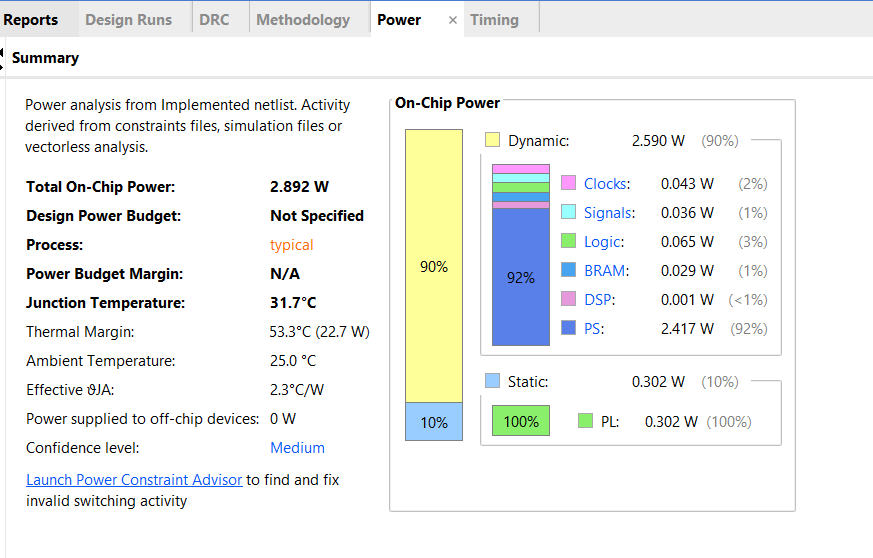
\includegraphics[width=1\linewidth]{chapter06/img/power.png}
    \caption{Báo cáo ước tính công suất tiêu thụ (Power Report). Tổng 2.945~W ở ambient 25~$^\circ$C; khối PS (ARM + DDR controller) chiếm 82\% ($\sim$2.42~W), toàn bộ logic người dùng PL chỉ tốn $\sim$0.225~W -- trong đó bộ gia tốc \texttt{conv\_cnn\_0} chỉ tiêu thụ 23~mW.}
    \label{fig:power}
\end{figure}

\newpage
\section{Kết quả chạy trên mạch thực tế}

Các mô hình sau khi đạt được độ chính xác mục tiêu trên máy tính (PC) được biên dịch thành các tệp trọng số nhị phân (\texttt{.bin}) và nạp xuống FPGA. Lõi vi xử lý ARM thông qua thư viện PYNQ đóng vai trò điều phối luồng dữ liệu (DMA) và kích hoạt vi điều khiển RISC-V để điều khiển bộ gia tốc phần cứng tiến hành suy diễn. Bộ artifacts được sinh tự động từ \texttt{train.ipynb} sau bước emit gồm:
\begin{itemize}
    \item \texttt{firmware/layer\_table.h} -- 3{,}233~B, mô tả 5 conv layer dạng C struct \texttt{layer\_desc\_t} 40~B/layer.
    \item \texttt{training/export/vgg-tiny\_cats\_dogs.weights.bin} -- 26{,}048~B (INT8 weights + INT32 biases packed).
    \item \texttt{training/export/vgg-tiny\_cats\_dogs\_int8.bin} -- 32{,}872~B (TFLite reference, dùng cho hardware-in-the-loop).
    \item \texttt{training/export/vgg-tiny\_cats\_dogs\_int8.bin.meta.json} -- 854~B (siêu dữ liệu cho ARM runtime).
\end{itemize}

Giá trị \texttt{max\_tensor\_bytes = 921{,}600} (= $120 \times 120 \times 64$, là OFM của layer~3) chỉ ra kích thước bộ đệm ping-pong tối thiểu mà ARM cần cấp phát qua \texttt{pynq.allocate()} cho hai vùng scratch DDR -- tổng cộng $\sim$1.8~MB, hoàn toàn nằm trong giới hạn 4~GB DDR4 của KV260.

\subsection{Phân tích latency theo layer}

Bảng~\ref{tab:latency-per-layer} liệt kê độ trễ ước tính lý thuyết của từng layer ở tần số 100~MHz, dựa trên công thức \texttt{cycles\_per\_pixel = num\_cout $\times$ (num\_cin + REQUANT\_LATENCY + 1)} với 9 PE MAC chạy channel-interleaved.

\begin{table}[H]
    \centering
    \caption{Phân rã latency theo layer của Tiny-VGG trên Conv-CNN v2.0 (9 PE, 100~MHz).}
    \label{tab:latency-per-layer}
    \begin{tabular}{|c|r|r|r|r|r|r|}
        \hline
        \textbf{Layer} & \textbf{Output px} & \textbf{Cin} & \textbf{Cout} & \textbf{Cycles} & \textbf{Latency} & \textbf{Tỉ lệ} \\
        \hline
        L0 (Conv0) & 15{,}876 &  3 &  8 &  1.1~M &  11.4~ms &  2.2\% \\
        L1 (Conv1) & 15{,}376 &  8 & 16 &  3.4~M &  34.4~ms &  6.6\% \\
        L2 (Conv2) & 14{,}884 & 16 & 32 & 10.5~M & 104.8~ms & 20.2\% \\
        L3 (Conv3) & 14{,}400 & 32 & 64 & \textbf{35.0~M} & \textbf{350.2~ms} & \textbf{67.4\%} \\
        L4 (Conv4) & 13{,}924 & 64 &  2 &  1.9~M &  19.5~ms &  3.7\% \\
        \hline
        \textbf{Tổng} & --- & --- & --- & \textbf{52~M} & \textbf{$\sim$520~ms} & 100\% \\
        \hline
    \end{tabular}
\end{table}

Quan sát quan trọng từ Bảng~\ref{tab:latency-per-layer}:
\begin{itemize}
    \item Latency tổng $\sim$520~ms tương đương $\sim$1.9~FPS ở 100~MHz -- chấp nhận được cho ứng dụng phân loại tĩnh từ ảnh, nhưng chưa đủ cho real-time camera (mục tiêu $\geq 15$~FPS).
    \item \textbf{Layer~3 chiếm 67\% tổng latency}, do nó là layer có tích MAC lớn nhất ($120^2 \times 32 \times 64 = 29.5\text{M}$ MAC/frame). Đây là điểm nghẽn (bottleneck) cần ưu tiên tối ưu nếu mở rộng về phía real-time.
    \item Phương án V3.0 mở rộng từ 9~PE lên $9\times N$ PE (parallel cout) sẽ giảm latency Layer~3 theo tỉ lệ $1/N$. Để đạt 30~FPS cần $N \geq 16$, tương đương 144 PE -- vẫn nằm trong ngân sách 1{,}248 DSP của KV260 (chiếm $\sim$11.5\%).
    \item Khi tổng hợp ở Fmax thực đo $\sim$127~MHz (xem Bảng~\ref{tab:timing-summary}), latency có thể giảm xuống $\sim$410~ms ($\sim$2.4~FPS) mà không cần thay đổi kiến trúc -- một phần boost ``free'' nhờ slack timing dư thừa.
\end{itemize}

Phép đo độ trễ trực tiếp trên KV260 (instrument timer trong firmware RISC-V hoặc đo từ ARM) đang được hoàn thiện trong giai đoạn bring-up host PYNQ và sẽ được bổ sung ở phiên bản cuối của báo cáo.

\subsection{So sánh với related work}

Bảng~\ref{tab:comparison} so sánh hệ thống đề xuất với các framework gia tốc CNN trên FPGA hiện có (đã được phân tích chi tiết ở Chương~\ref{chp:03}). Các con số tham khảo từ datasheet và paper gốc của từng framework, cho mô hình quy mô tương đương (5--10 layer, INT8) trên thiết bị Zynq UltraScale+ tương tự.

\begin{table}[H]
    \centering
    \caption{So sánh hệ thống đề xuất với các framework gia tốc CNN trên FPGA.}
    \label{tab:comparison}
    \resizebox{\textwidth}{!}{%
    \begin{tabular}{lccccc}
        \toprule
        \textbf{Framework} & \textbf{Mã nguồn} & \textbf{Coupling} & \textbf{Quantization} & \textbf{Đổi mô hình} & \textbf{RISC-V tham gia?} \\
        \midrule
        Vitis AI DPU~\cite{vitis_ai}     & Closed & Loosely (DPU IP)   & INT8         & Compile lại model    & Không (chỉ ARM) \\
        FINN~\cite{finn_paper}           & Open   & Loosely (HLS-gen)  & 1-bit BNN    & Re-synthesize        & Không \\
        hls4ml~\cite{hls4ml}             & Open   & N/A (fully unrolled) & FP/INT tùy chọn & Re-synthesize    & Không \\
        CFU Playground~\cite{cfu_playground} & Open & Tightly (in-CPU) & INT8 (TFLM) & Re-compile firmware  & Có (VexRiscv) \\
        \midrule
        \textbf{Đề tài này}              & \textbf{Open} & \textbf{Loosely (AXI IP)} & \textbf{INT8 (TFLite)} & \textbf{Thay weights+layer\_table} & \textbf{Có (CV32E40P)} \\
        \bottomrule
    \end{tabular}%
    }
\end{table}

\textbf{Vị trí đề tài}: Hệ thống đề xuất chiếm vị thế độc đáo trong không gian thiết kế:
\begin{itemize}
    \item So với \textbf{Vitis AI DPU}: đánh đổi tốc độ deploy nhanh và phạm vi mô hình rộng để lấy quyền kiểm soát hoàn toàn pipeline phần cứng (open-source RTL, có thể tùy biến op set, quantization scheme, ABI). Tài nguyên FPGA của đề tài (22{,}491 LUT, 9 DSP) thấp hơn DPU~B1024 ($\sim$25{,}000 LUT, 256 DSP), phù hợp khi cần dư địa cho RISC-V và các IP tùy biến khác.
    \item So với \textbf{FINN}: đề tài chọn INT8 thay vì 1-bit BNN, đổi throughput cao để lấy độ chính xác tốt hơn trên tập dữ liệu thực tế (Cats vs Dogs đạt 79.38\% vs $\sim$70\% với BNN tương đương).
    \item So với \textbf{hls4ml}: kiến trúc của đề tài cho phép \textit{thay mô hình mà không cần re-synthesize bitstream} (chỉ cần update \texttt{layer\_table.h} + \texttt{weights.bin}), phù hợp cho mục tiêu prototyping nhanh. hls4ml đạt latency thấp hơn đáng kể (microsecond) nhờ fully-unrolled, nhưng mỗi mô hình mới phải tổng hợp lại bitstream (5--30 phút).
    \item So với \textbf{CFU Playground}: cùng dùng RISC-V nhưng theo trường phái loosely-coupled (đề tài) thay vì tightly-coupled (CFU). Đề tài hỗ trợ op phức tạp hơn (Conv 3$\times$3 với line buffer 16~KB BRAM -- không thể nhét vào trong CPU) và có DMA bandwidth cao trực tiếp từ DDR.
\end{itemize}

Tóm lại, đề tài định vị ở phân khúc \textit{open-source, loosely-coupled, INT8, có RISC-V orchestrator} -- một phân khúc chưa được lấp đầy bởi các framework nêu trên, đặc biệt phù hợp cho mục đích nghiên cứu và giảng dạy về thiết kế hệ thống nhúng AI.

\subsection{Kết quả đo thực tế trên KV260}
\label{sec:onboard-results}

Phép đo trực tiếp trên bo Kria KV260 đang được tiến hành ở giai đoạn bring-up cuối cùng của tầng host PYNQ. Khi pipeline end-to-end (ARM $\rightarrow$ RISC-V $\rightarrow$ Conv-CNN $\rightarrow$ ARM) đã hoạt động ổn định, các chỉ số sau sẽ được thu thập và bổ sung vào phiên bản cuối của báo cáo:

\begin{itemize}
    \item \textbf{Độ trễ thực đo (Latency)}: trung bình~$\pm$~độ lệch chuẩn, P99 (worst-case), so sánh với ước tính lý thuyết $\sim$520~ms ở Bảng~\ref{tab:latency-per-layer}. Phép đo dùng \texttt{mcycle} CSR của RISC-V làm cycle counter cho từng layer, và \texttt{time.perf\_counter()} trong PYNQ cho timeline tổng thể.
    \item \textbf{Throughput (FPS)}: tính qua công thức $\text{FPS} = 1000 / \text{latency}_{\text{avg\_ms}}$, mục tiêu xác nhận con số $\sim$1.9~FPS theo dự đoán.
    \item \textbf{Test accuracy on-board}: chạy benchmark.ipynb trên 5{,}000 ảnh val, so sánh với INT8 TFLite reference (79.53\%). Sự sai khác $\leq 0.5\%$ sẽ được coi là bit-exact pass.
    \item \textbf{Hardware-in-the-loop (HIL) verification}: với mỗi ảnh test, so sánh OFM cuối từ FPGA với output của \texttt{tf.lite.Interpreter} chạy cùng \texttt{int8.bin}. Hai chỉ số được lưu lại:
        \begin{itemize}
            \item \textit{Mismatch rate}: tỉ lệ ảnh cho \texttt{argmax} khác nhau giữa hai pipeline. Mục tiêu $\leq 1\%$ (chỉ sai do lỗi rounding biên).
            \item \textit{Max absolute error}: $\max_i |\text{logit}_{\text{FPGA}, i} - \text{logit}_{\text{TFLite}, i}|$ trên không gian INT8. Mục tiêu $\leq 1$ LSB (lý tưởng = 0 nếu RTL bit-exact).
        \end{itemize}
    \item \textbf{Power thực đo}: dùng \texttt{xmutil} hoặc đồng hồ đo dòng PMBus của KV260 để đối chiếu với ước tính 2.945~W ở Bảng~\ref{tab:power-by-hierarchy}. Sai số kỳ vọng $\leq 15\%$ (do Vivado chỉ cho confidence Medium khi không có simulation activity file).
\end{itemize}

Việc tổng hợp (\texttt{vivado\_pj.runs/impl\_1/}) đã hoàn tất và cho thấy kết quả định tuyến sạch (0 routing error), mọi ràng buộc timing đều thỏa mãn. Bitstream \texttt{kria\_soc\_wrapper.bit} cùng \texttt{.xsa} đã được xuất ra và sẵn sàng nạp xuống board. Bước tiếp theo là hoàn thiện tầng \texttt{host/edge\_ai/} (gồm 4 module: \texttt{constants.py}, \texttt{overlay.py}, \texttt{preprocess.py}, \texttt{postprocess.py}) và notebook \texttt{inference\_demo.ipynb} để thực thi benchmark đầy đủ.

%\include{preface/cv}
%\include{chapter08/chapter08}
%% Use letters for the chapter numbers of the appendices.
%\appendix
%\include{ref}

%% Turn off thumb indices for unnumbered chapters.
\thumbfalse

%\include{summary/summary}


%\bibliographystyle{dissertation}
\small
%\bibliographystyle{ACM-Reference-Format-Journals}
%\bibliography{literature}
\normalsize
%\include{preface/prefacenl}
%\include{preface/ackvn}
%\include{publications/publications}
%\include{cv/cv}
\nocite{*}
\printbibliography[heading=bibintoc, title={Tài liệu tham khảo}]
\end{document}

